\documentclass[11pt,a4paper,oneside]{report}

\usepackage[T1]{fontenc}
\usepackage[utf8]{inputenc}
\usepackage[british]{babel}

\usepackage[margin=23mm, headheight=15pt, includehead, includefoot]{geometry}

\usepackage{lmodern}
\usepackage{microtype}
\usepackage{enumitem}
\usepackage{setspace}
\usepackage{parskip}

\setstretch{1.045}
\setlength{\parindent}{0pt}
\setlength{\parskip}{0.58em}

\clubpenalty=10000
\widowpenalty=10000
\displaywidowpenalty=10000

\usepackage{amsmath}
\usepackage{amssymb}
\usepackage{mathtools}
\usepackage{bm}
\usepackage{siunitx}

\sisetup{
    detect-all,
    separate-uncertainty=true,
    range-phrase={--},
    range-units=single
}

\usepackage{booktabs}
\usepackage{tabularx}
\usepackage{array}
\usepackage{longtable}
\usepackage{multirow}
\usepackage{makecell}

\newcolumntype{Y}{>{\raggedright\arraybackslash}X}
\newcolumntype{C}[1]{>{\centering\arraybackslash}p{#1}}
\newcolumntype{L}[1]{>{\raggedright\arraybackslash}p{#1}}

\usepackage{graphicx}
\usepackage{float}
\usepackage{caption}
\usepackage{subcaption}

\usepackage{tikz}
\usepackage{pgfplots}
\pgfplotsset{compat=1.18}

\usetikzlibrary{
    arrows.meta,
    positioning,
    calc,
    fit,
    backgrounds,
    shapes.geometric,
    patterns,
    matrix
}

\usepackage[many]{tcolorbox}

\definecolor{geoBlue}{RGB}{20, 45, 85}
\definecolor{geoLight}{RGB}{240, 244, 250}
\definecolor{geoMid}{RGB}{180, 195, 215}
\definecolor{geoDark}{RGB}{15, 25, 45}
\definecolor{geoGold}{RGB}{185, 140, 45}
\definecolor{geoGoldLight}{RGB}{252, 248, 235}
\definecolor{geoGreen}{RGB}{35, 120, 75}
\definecolor{geoGreenLight}{RGB}{235, 248, 240}
\definecolor{geoRust}{RGB}{175, 55, 40}
\definecolor{geoRedLight}{RGB}{253, 242, 240}
\definecolor{geoGrey}{RGB}{100, 110, 120}
\definecolor{geoTeal}{RGB}{30, 130, 140}

\newtcolorbox{governingrule}[1][Governing rule]{enhanced, breakable, colback=geoLight, colframe=geoBlue, boxrule=0.7pt, arc=1.5mm, left=3mm, right=3mm, top=2.5mm, bottom=2.5mm, title=\textbf{#1}, fonttitle=\color{white}, colbacktitle=geoBlue}

\newtcolorbox{claimboundary}[1][Claim boundary]{enhanced, breakable, colback=geoGoldLight, colframe=geoGold, boxrule=0.7pt, arc=1.5mm, left=3mm, right=3mm, top=2.5mm, bottom=2.5mm, title=\textbf{#1}, fonttitle=\color{geoDark}, colbacktitle=geoGold}

\newtcolorbox{engineeringconsequence}[1][Engineering consequence]{enhanced, breakable, colback=geoGreenLight, colframe=geoGreen, boxrule=0.7pt, arc=1.5mm, left=3mm, right=3mm, top=2.5mm, bottom=2.5mm, title=\textbf{#1}, fonttitle=\color{white}, colbacktitle=geoGreen}

\newtcolorbox{reviewerquestion}[1][Reviewer question]{enhanced, breakable, colback=geoRedLight, colframe=geoRust, boxrule=0.7pt, arc=1.5mm, left=3mm, right=3mm, top=2.5mm, bottom=2.5mm, title=\textbf{#1}, fonttitle=\color{white}, colbacktitle=geoRust}

\newtcolorbox{evidencebox}[1][Evidence state]{enhanced, breakable, colback=white, colframe=geoGrey, boxrule=0.6pt, arc=1.5mm, left=3mm, right=3mm, top=2.5mm, bottom=2.5mm, title=\textbf{#1}, fonttitle=\color{white}, colbacktitle=geoGrey}

\usepackage{fancyhdr}
\pagestyle{fancy}
\fancyhf{}
\fancyhead[L]{\scriptsize\color{geoGrey}CHAPTER \thechapter}
\fancyhead[R]{\small\color{geoGrey}Geatomica Public Evidence Edition}
\fancyfoot[C]{\small\color{geoGrey}\thepage}
\renewcommand{\headrulewidth}{0.4pt}
\renewcommand{\footrulewidth}{0pt}

\fancypagestyle{plain}{
    \fancyhf{}
    \fancyfoot[C]{\small\color{geoGrey}\thepage}
    \renewcommand{\headrulewidth}{0pt}
}

\usepackage{titlesec}

\titleformat{\chapter}[display]
    {\normalfont\bfseries\color{geoBlue}}
    {\filleft\Large\color{geoGold}\chaptername\ \thechapter}
    {0.4em}
    {\titlerule[1pt]\vspace{0.65em}\Huge}
    [\vspace{0.4em}\titlerule]

\titlespacing*{\chapter}{0pt}{-15pt}{28pt}

\titleformat{\section}{\Large\bfseries\color{geoBlue}}{\thesection}{0.65em}{}
\titlespacing*{\section}{0pt}{1.5ex plus .5ex minus .2ex}{1ex plus .2ex}

\titleformat{\subsection}{\large\bfseries\color{geoDark}}{\thesubsection}{0.55em}{}
\titlespacing*{\subsection}{0pt}{1.2ex plus .4ex minus .2ex}{0.8ex plus .2ex}

\titleformat{\subsubsection}{\normalsize\bfseries\color{geoDark}}{\thesubsubsection}{0.45em}{}
\titlespacing*{\subsubsection}{0pt}{1ex plus .3ex minus .2ex}{0.6ex plus .2ex}

\usepackage[
    colorlinks=true,
    linkcolor=geoBlue,
    citecolor=geoGreen,
    urlcolor=geoBlue,
    bookmarks=true,
    bookmarksnumbered=true,
    pdftitle={Geatomica: Public Evidence Edition v1.0.1},
    pdfauthor={Joseph Maxwell},
    pdfsubject={Materials assurance, descriptor authority, model viability and execution evidence},
    pdfkeywords={Geatomica, materials informatics, model assurance, descriptor authority, reproducibility}
]{hyperref}


\providecommand{\accepted}{\textcolor{geoGreen}{\textbf{[ACCEPTED]}}}
\providecommand{\bounded}{\textcolor{geoGold}{\textbf{[BOUNDED]}}}
\providecommand{\hold}{\textcolor{geoRust}{\textbf{[HOLD]}}}
\providecommand{\refuse}{\textcolor{geoRust}{\textbf{[REFUSE]}}}
\providecommand{\sourcehold}{\textcolor{geoRust}{\textbf{[SOURCE HOLD]}}}
\providecommand{\replayhold}{\textcolor{geoRust}{\textbf{[REPLAY HOLD]}}}
\providecommand{\term}[1]{\textbf{#1}}
\providecommand{\Rtwo}{\ensuremath{R^2}}
\providecommand{\Stwo}{\ensuremath{S^2}}
\providecommand{\Rnull}{\ensuremath{R^2_{\mathrm{null}}}}
\providecommand{\Rvalid}{\ensuremath{R^2_{\mathrm{valid}}}}
\newcommand{\authorcheck}[1]{}
\begin{document}
\pagenumbering{roman}
\begin{titlepage}



\thispagestyle{empty}



\begin{center}



\vspace*{0.8cm}



{\small

\bfseries

\color{geoGold}

GEATOMICA

\,|\,

MATERIALS ASSURANCE

\,|\,

    PUBLIC EVIDENCE EDITION V1.0.1 \textbar{} OCTOBER 2026

\par}



\vspace{0.85cm}



{\Huge

\bfseries

\color{geoBlue}

Geatomica

\par}



\vspace{0.22cm}



{\LARGE

\bfseries

\color{geoDark}

A Materials Assurance Framework for

Descriptor Authority,

Model Viability

and Engineering Trust

\par}



\vspace{0.55cm}



{\large

A failure-first,

cross-source study of materials data,

models,

explanations

and the decisions built around them

\par}



\vspace{0.9cm}



{\Large

\textbf{Joseph Maxwell}

\par}



\vspace{0.18cm}



{\normalsize

The Systemica Institute, London, United Kingdom

\par}



\vspace{0.18cm}



{\small

\texttt{j.maxwell@systemicainstitute.org}

\par}



\vspace{0.95cm}



% ------------------------------------------------------------

% TITLE-PAGE PROGRAMME FIGURE

% ------------------------------------------------------------



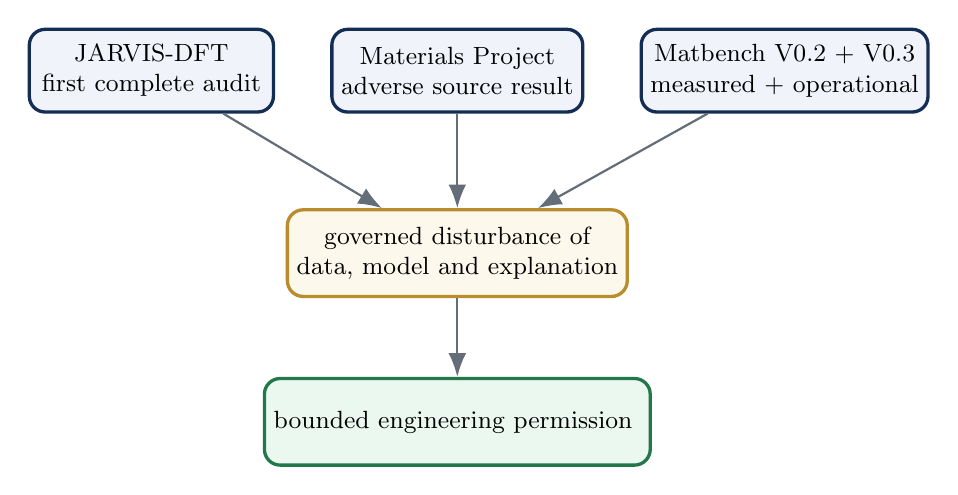
\begin{tikzpicture}[node distance=8mm and 7mm, every node/.style={ font=\small, align=center }, source/.style={ draw=geoBlue, very thick, rounded corners=2mm, fill=geoLight, minimum width=3.1cm, minimum height=1.05cm }, process/.style={ draw=geoGold, very thick, rounded corners=2mm, fill=geoGoldLight, minimum width=4.2cm, minimum height=1.1cm }, outcome/.style={ draw=geoGreen, very thick, rounded corners=2mm, fill=geoGreenLight, minimum width=4.2cm, minimum height=1.1cm }]
\node[source] (jarvis) {
    JARVIS-DFT\\
    first complete audit
};
\node[source, right=of jarvis] (mp) {
    Materials Project\\
    adverse source result
};
\node[source, right=of mp] (matbench) {
    Matbench V0.2 + V0.3\\
measured + operational
};
\node[
    process,
    below=12mm of mp
] (audit) {
    governed disturbance of\\
    data, model and explanation
};
\node[
    outcome,
    below=10mm of audit
] (authority) {
    bounded engineering permission
};
\draw[
    -{Latex[length=3mm]},
    thick,
    color=geoGrey
]
(jarvis) -- (audit);
\draw[
    -{Latex[length=3mm]},
    thick,
    color=geoGrey
]
(mp) -- (audit);
\draw[
    -{Latex[length=3mm]},
    thick,
    color=geoGrey
]
(matbench) -- (audit);
\draw[
    -{Latex[length=3mm]},
    thick,
    color=geoGrey
]
(audit) -- (authority);
\end{tikzpicture}



\vfill



\begin{minipage}{0.90\textwidth}



\small



\textbf{\color{geoBlue}Scientific evidence state.}



This evidence edition integrates:
\begin{itemize}
\item a JARVIS-DFT four-target audit and numerically equivalent local replay, with raw-byte divergence preserved;
\item a Materials Project programme whose energetic/electronic evidence remains bounded and whose raw elastic interpretation remains on source hold;
\item a completed CPU Matbench V0.2 nomination run containing 20 valid official-fold units and paired permutation-target nulls;
\item a sealed 3,440-unit Matbench V0.3 fresh assurance run with exact same-environment repeat completed;
\item a sealed Spatial V0.5 factorial replay and a final Spatial V0.6.1 confirmation in which 576 fresh and 576 replay units were byte-, metadata- and numerically identical; bulk metric geometry confirmed while shear polarity remained conditional.
\end{itemize}
The demonstrated scientific evidence is materials-specific; the runtime, replay, memory and authority contracts are formulated independently of materials semantics, making cross-domain transfer a testable successor hypothesis rather than a present validation claim.

The manuscript reports measured, replayed, report-bound and operational evidence as separate classes. It is not peer reviewed, does not authorise material selection or qualification, and does not claim universal descriptor hierarchy, physical causality, experimental validation or external validation.



\end{minipage}



\vspace{0.6cm}



{\small

    October 2026

\,|\,

    Corrected preprint successor to archived v1.0.0

}



\end{center}



\end{titlepage}



% ============================================================

% AUTHORSHIP AND STATUS PAGE

% ============================================================




\clearpage
\chapter*{Authorship, Evidence and Publication Status}
\addcontentsline{toc}{chapter}{Authorship, Evidence and Publication Status}

Joseph Maxwell is the sole human author and research lead of the Geatomica research
programme. AI and coding systems assisted implementation, critique, evidence organisation and document production under author review. They do not hold scientific or publication authority.

Statements are classified as \textbf{MEASURED LOCAL}, \textbf{REPLAYED LOCAL},
\textbf{HISTORICAL/\allowbreak REPORT-BOUND}, \textbf{READ-ONLY DERIVED},
\textbf{INTERPRETATION} or \textbf{PLANNED}. A lower class cannot overwrite raw
output or a sealed receipt.

Preprint status: final Spatial V0.6.1 replay integrated. This document is not peer reviewed and makes no external-validation claim.

\textbf{Revision status.} Version 1.0.1 is a maintained successor to the deposited v1.0.0 manuscript. It corrects a documentation-only preprocessing statement, narrows one figure caption, distinguishes two differently bounded percentages, and updates repository navigation. No model was rerun and no accepted numerical result, table or protocol was changed for this revision.

\clearpage
\chapter*{Abstract}
\addcontentsline{toc}{chapter}{Abstract}

Materials models can be predictively useful while remaining unsuitable as
explanations or engineering authorities. Geatomica separates source admission,
absolute model viability, null separation, descriptor-response stability,
representation adequacy, replay and promotion authority.

The evidence programme now includes a JARVIS four-target carrier audit with
numerically equivalent local replay; an adverse Materials Project elastic
admission result; sealed 3,440-unit Matbench V0.3 fresh and repeat runs with
65,740 compared numeric cells exactly equal;
and a sealed, byte-identical Spatial GIL 256 replay. Matbench V0.3 retained strong
predictive signal across formation energy, band gap, logarithmic bulk modulus and
logarithmic shear modulus. Yet fitted permutation rankings and retrained-removal
consequences were almost uncorrelated on average (Spearman approximately 0.039),
with only 10 percent mean top-10 overlap. Because the protocol lacks sham
full-feature refits, this disagreement establishes that fitted importance cannot
be treated as necessity but does not uniquely partition redundancy from
optimisation variation.

Spatial GIL first tested whether a complete-shell six-bin angle summary preserved
the advantage seen in an earlier 64-material split; it did not. A factorial
decomposition then isolated continuous metric geometry as the strongest compact
block. In the final V0.6.1 confirmation, bulk metric geometry passed continuity and
zero chemical-system-overlap views, while shear polarity failed the required
cross-view confirmation. Fresh and replay executions each sealed 576 units; all
1,728 corresponding output files and 927,361 numeric cells were exactly identical.
Replay therefore preserved both the positive and held decisions.

The current contribution is bounded local computational evidence. It does not
establish causal descriptor hierarchy, engineering qualification, physical or
external validation, or external replication.

\clearpage

\chapter*{Reader Map}
\addcontentsline{toc}{chapter}{Reader Map}
\begin{center}
\fbox{\parbox{0.91\textwidth}{\textbf{This monograph in plain language.} \textbf{Question:} what remains trustworthy when materials-ML evidence is challenged at its source, model, representation, or execution boundary? \textbf{What we did:} we tested those boundaries across JARVIS, Materials Project, Matbench, Spatial, and three bounded engineering studies. \textbf{What we found:} fitted use, retrained dependence, null separation, absolute prediction, replay, and permission to act are not interchangeable. \textbf{Boundary:} the evidence is local and computational; it is not external replication, physical qualification, or universal engineering authority.}}
\end{center}

\textbf{Three reading levels.} \textbf{Just want the answer?} Read this box, the evidence boxes in Chapters 4--8, and the Conclusion. \textbf{Want the experiments?} Read Chapters 3--8. \textbf{Want to audit the programme?} Use Appendices A--D, the public evidence package, and the route-specific receipts.

\textbf{If you have five minutes.} Read the Abstract, the five-line evidence boxes at the start of Chapters 4--8, and the Conclusion. They state the question, comparison, result, decision, and boundary for each empirical route.

\textbf{If you are reviewing the scientific claims.} Chapter 3 defines the programme and its decision rules. Chapters 4--8 contain the measured JARVIS, Materials Project, Matbench, and Spatial results. Appendix C records replay and runtime states. Appendix D gives the claim-relevant scientific configurations.

\textbf{If you are evaluating descriptor interpretation.} Start with Chapter 2, then read Chapters 4, 6, 7, and 8. The central distinction is between what a fitted model uses and what the learning problem can replace after removal and retraining.

\textbf{If you are evaluating model usefulness.} Read Chapter 5 first. It shows why beating a target-permutation null did not imply positive held-out predictive performance for the Materials Project elastic route.

\textbf{If you are evaluating reproducibility.} Read Chapters 8 and 12 and Appendix C. Fresh execution, resume, and replay are kept separate. Byte, semantic, and numerical agreement are reported independently where available.

\textbf{If you are evaluating engineering relevance.} Read Chapters 11--13. The furnace, dual-tank, and heat-shield studies are bounded evidence-to-next-test cases, not deployment validation.

\textbf{If you are evaluating general-engineering transfer.} Read the engineering-witness chapter, the runtime chapter, and the separate Technical \& Industrial Companion. The engineering cases provide local control-logic witnesses; they are not retrospective full-stack deployments.

\textbf{If you are evaluating methods.} Appendix D consolidates the claim-relevant datasets, representations, splits, preprocessing, models, seeds, nulls, thresholds, and replay contracts. Private reusable orchestration is not required to inspect these scientific configurations.

\begin{center}
\fbox{\parbox{0.91\textwidth}{\textbf{Programme in one sentence.} The work tests whether apparently useful materials-ML evidence remains useful when the source, population, representation, model interpretation, or execution state is challenged, and it refuses to let a weaker result stand in for a stronger one.}}
\end{center}

\tableofcontents
\clearpage
\listoffigures
\clearpage
\listoftables
\clearpage

\pagenumbering{arabic}
\chapter{Introduction}



\label{chap:introduction}



\section{Materials engineering begins after the event}



Materials engineers rarely receive the process they need to

understand.



They receive what remains after the process has already happened.



A polished and etched microstructure after solidification,

heat treatment

and deformation.



A fracture surface after the applied force has gone and the crack has

stopped moving.



A coating after oxidation,

thermal cycling

or local delamination.



A failed component after manufacturing history,

service conditions

and geometry have combined into one final state.



The evidence is real.



It is also incomplete.



A micrograph does not arrive with labels identifying every thermal

hold,

cooling rate,

contaminant,

stress concentration

or local transformation that produced it.



A fracture surface can constrain the loading history without narrating

that history by itself.



The engineer therefore works backwards.



Possible histories are proposed,

then tested against whatever else those histories should have left

behind.



If fatigue dominated,

should repeated growth markings be present?



If thermal shock initiated the crack,

what temperature gradient and local constraint would have been

required?



If processing caused a brittle microstructure,

which phases,

grain morphologies

or residual stresses should accompany it?



The best explanation is not the story that fits one mark most

beautifully.



It is the history that survives the greatest number of independent

constraints.



This reconstructive logic sits beneath much of materials science.



Composition names the ingredients.



Processing determines what those ingredients become.



Structure records part of that history.



Properties describe how the surviving structure responds.



Failure reveals one of the routes by which the available margin was

lost.



\begin{governingrule}



A surviving structure is evidence of the process that produced it.



It is not the process in full.



\end{governingrule}



Machine-learning outputs deserve the same discipline.



A fitted model is another surviving structure.



Its final score,

feature ranking

and predictions are the visible endpoint of decisions made earlier:

what source was queried,

which records were admitted,

which variables were available,

how values were transformed,

where the population was split,

which model family was selected,

what objective was optimised

and which failures were allowed to disappear inside an aggregate.



The model output remains real.



The problem begins when the finished structure is mistaken for a

transparent account of the material system itself.



\section{From prediction to engineering consequence}



Materials informatics has made predictive modelling easier to access

and easier to compare.



Large calculated databases expose formation energies,

electronic properties,

structures

and mechanical responses at scales that would be impractical to

reproduce experimentally.



Benchmark suites provide consistent tasks and evaluation procedures.



Composition descriptors,

structural representations,

graph models

and increasingly large learned representations can produce strong

property predictions.



That progress matters.



The engineering risk does not arise because prediction is useless.



It arises because a predictive result can quietly acquire a stronger

meaning than the experiment actually established.



A feature importance ranking may be narrated as a physical mechanism.



A high \Rtwo{} may be treated as evidence that the model is safe to

use outside the population on which it was tested.



A populated database field may be treated as scientifically

admissible because the source itself is respected.



A repeated top descriptor may be assumed to be necessary.



A model that beats a null may be promoted even when its absolute

predictions remain unusable.



Each move begins with genuine evidence.



The overreach occurs in the reconstruction built around it.



This matters because a model does not remain inside a notebook.



It can change what an engineer does next.



A promoted descriptor may influence:



\begin{itemize}



\item

which material variable is measured routinely;



\item

which high-fidelity calculation is commissioned;



\item

which alloy or ceramic family is screened first;



\item

which experiment receives time and budget;



\item

which physical interpretation enters a design discussion;



\item

which route is rejected before fabrication;



\item

which uncertainty is no longer investigated because the model appears

settled.



\end{itemize}



A descriptor therefore gains practical authority when it begins to

change decisions.



That authority should not be inherited automatically from predictive

performance.



\begin{engineeringconsequence}



The important engineering question is not only:



\emph{Which model predicts best?}



It is:



\emph{Which part of the model's account is reliable enough to justify the next expensive action, and under what conditions should that permission stop?}



\end{engineeringconsequence}



This is the problem addressed by Geatomica.



It is a materials-assurance problem before it is a software-governance

problem.



The software exists because the scientific question could not be

answered reliably without controlling the route that produced the

evidence.



\section{How the research question changed}



Geatomica did not begin as a general assurance framework.



It began as a materials-informatics question.



Could a small set of governing descriptors explain enough of a

material response to reduce modelling complexity without cutting away

the underlying physics?



The initial physical intuition was straightforward.



Macroscopic mechanical properties do not arise independently of

bonding,

electronic state,

energetic organisation,

structure

and packing.



If some descriptors sit upstream of several material responses,

then relationships involving those descriptors might persist across

changes in model,

population

or representation.



Such persistence could support reduced-complexity modelling,

better measurement prioritisation

and clearer escalation to more expensive calculations.



The first obstacle was feature importance.



A fitted model could produce a plausible ranking,

but the ranking answered only where that model routed information

under one data state.



It did not establish whether the relationship survived another model,

another split,

another population

or complete retraining without the feature.



The question changed:



\begin{quote}



Can descriptor stability be measured across controlled changes in the

modelling process?



\end{quote}



The next obstacle was that stability itself remained insufficient.



A descriptor might recur across seeds or perturbations while the

underlying model remained absolutely unusable.



An apparently stable ranking might also emerge from an inadmissible

target population.



A model could preserve ordering while failing a strict replay

contract.



The question changed again:



\begin{quote}



When is the evidence surrounding a descriptor strong enough for it to

influence an engineering decision?



\end{quote}



This sequence produced the concept of

\term{descriptor authority}.



Authority is not another name for importance or stability.



It is bounded permission derived from several evidence objects that

must remain distinguishable.



Figure~\ref{fig:question-evolution}

summarises how the research programme evolved.



% ------------------------------------------------------------

% FIGURE 1.1

% EVOLUTION OF THE RESEARCH QUESTION

% ------------------------------------------------------------



\begin{figure}[H]



\centering



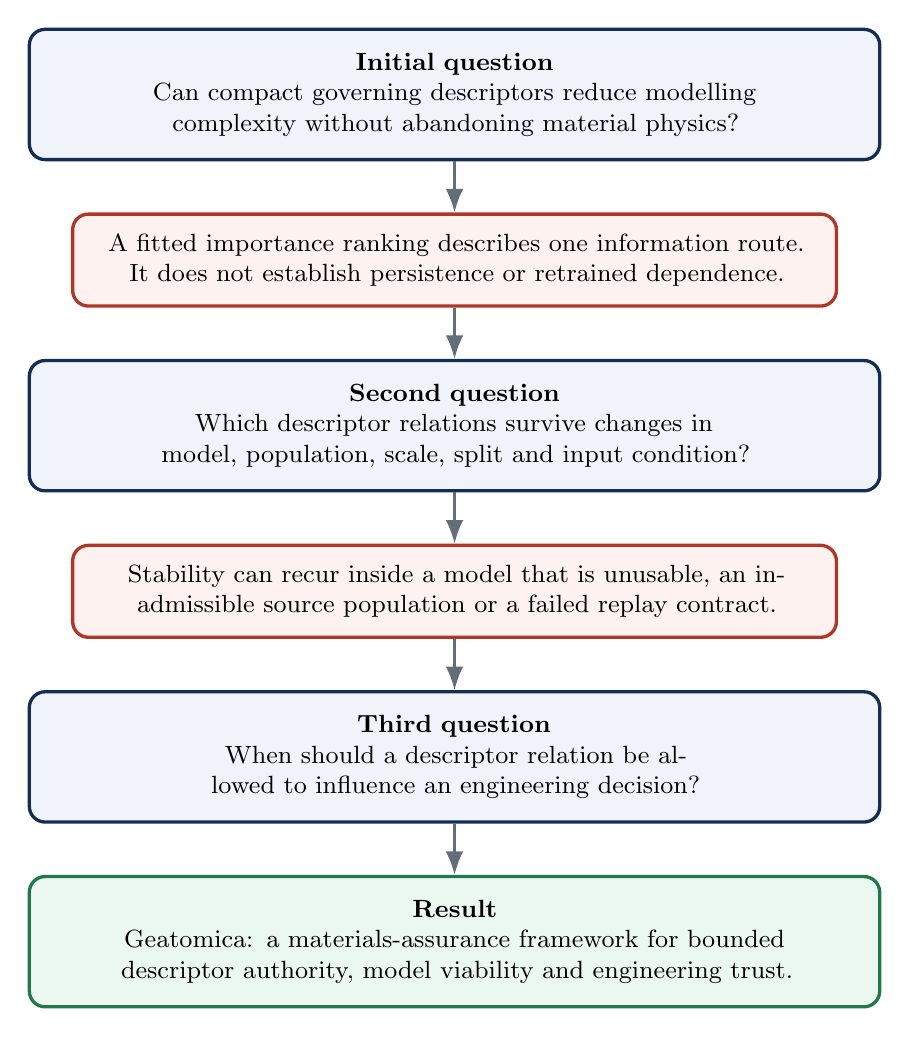
\begin{tikzpicture}[node distance=6.5mm, every node/.style={ font=\small, align=center }, qnode/.style={ draw=geoBlue, very thick, rounded corners=2mm, fill=geoLight, text width=10.2cm, minimum height=1.0cm, inner sep=3mm }, finding/.style={ draw=geoRust, very thick, rounded corners=2mm, fill=geoRedLight, text width=9.2cm, minimum height=0.9cm, inner sep=2.5mm }, result/.style={ draw=geoGreen, very thick, rounded corners=2mm, fill=geoGreenLight, text width=10.2cm, minimum height=1.0cm, inner sep=3mm }]
\node[qnode] (q1) {
    \textbf{Initial question}\\
    Can compact governing descriptors reduce modelling complexity
    without abandoning material physics?
};
\node[
    finding,
    below=of q1
] (f1) {
    A fitted importance ranking describes one information route.
    It does not establish persistence or retrained dependence.
};
\node[
    qnode,
    below=of f1
] (q2) {
    \textbf{Second question}\\
    Which descriptor relations survive changes in model,
    population,
    scale,
    split
    and input condition?
};
\node[
    finding,
    below=of q2
] (f2) {
    Stability can recur inside a model that is unusable,
    an inadmissible source population
    or a failed replay contract.
};
\node[
    qnode,
    below=of f2
] (q3) {
    \textbf{Third question}\\
    When should a descriptor relation be allowed to influence an
    engineering decision?
};
\node[
    result,
    below=of q3
] (r1) {
    \textbf{Result}\\
    Geatomica:
    a materials-assurance framework for bounded descriptor authority,
    model viability
    and engineering trust.
};
\draw[
    -{Latex[length=3mm]},
    thick,
    color=geoGrey
]
(q1) -- (f1);
\draw[
    -{Latex[length=3mm]},
    thick,
    color=geoGrey
]
(f1) -- (q2);
\draw[
    -{Latex[length=3mm]},
    thick,
    color=geoGrey
]
(q2) -- (f2);
\draw[
    -{Latex[length=3mm]},
    thick,
    color=geoGrey
]
(f2) -- (q3);
\draw[
    -{Latex[length=3mm]},
    thick,
    color=geoGrey
]
(q3) -- (r1);
\end{tikzpicture}



\caption{Evolution of the Geatomica research question. The framework did not begin as an abstract governance architecture. Each additional layer was introduced because the preceding evidence object proved insufficient for the engineering decision being asked of it.}



\label{fig:question-evolution}



\end{figure}



The framework is therefore best understood as an experimental

consequence.



Evidence admission became necessary because available records were not

automatically interpretable.



Null testing became necessary because predictive performance could be

manufactured by leakage or weak controls.



Absolute viability became necessary because beating a null did not

guarantee useful prediction.



Descriptor disturbance became necessary because one fitted ranking

could not establish persistence.



Retrained removal became necessary because fitted reliance did not

establish retrained dependence or physical necessity.



Replay became necessary because one completed execution did not

establish reproducibility.



Recovery became necessary because long-running audits could be

interrupted without invalidating every completed scientific unit.



Governance became necessary because mixed evidence states could not be

represented honestly by one terminal success label.



The architecture grew around the scientific problem.



It should not replace it as the centre of the manuscript.



\section{The central distinction: importance, stability and authority}



The word \emph{important} is routinely used for several different

questions.



Geatomica separates at least three.



\begin{table}[H]



\centering



\caption{The three principal evidence objects separated by Geatomica.}



\label{tab:three-evidence-objects}



\begin{tabularx}{\textwidth}{L{0.19\textwidth}
    Y
    Y
}
\toprule
\textbf{Evidence object}
&
\textbf{Operational question}
&
\textbf{What it does not establish}
\\
\midrule
\term{Predictive importance}
&
Where did this fitted model route information under this exact
dataset,
representation,
learner
and evaluation state?
&
Physical necessity,
transfer,
causality,
robustness
or engineering permission.
\\
\addlinespace
\term{Transformation stability}
&
Does a declared descriptor statistic remain within stated bounds when
the allowed modelling conditions are changed?
&
Absolute model usefulness,
source admissibility,
causality
or truth outside the tested transformation family.
\\
\addlinespace
\term{Descriptor authority}
&
Is the combined evidence sufficient to permit use of the descriptor
relation for a declared claim or engineering action within an
evidenced domain?
&
Universal validity,
material qualification
or truth outside that bounded domain.
\\
\bottomrule
\end{tabularx}



\end{table}



A descriptor can be highly important and fragile.



It can be weakly ranked but difficult to replace.



It can recur across seeds while collapsing under a chemical-system

holdout.



It can survive within one source while failing in another.



It can remain stable while the carrier model fails absolute viability.



It can appear physically plausible while the source records themselves

are inadmissible.



These are not contradictions to be averaged away.



They are different measurements of how the reconstruction was built.



\begin{reviewerquestion}[Why is descriptor authority not simply feature stability plus an applicability domain?]



Feature stability,

applicability domains,

uncertainty estimation,

feature importance,

negative controls

and reproducibility each measure part of the problem.



Geatomica's contribution is not to rename those parts.



It is to preserve their distinctions,

measure their disagreement

and prevent one evidence object from impersonating another.



An applicability domain may identify where prediction is reliable

without establishing that the same explanation remains reliable.



A stable feature ranking may recur while the model remains worse than

the mean baseline.



A numerically replayable result may still originate from an

inadmissible source population.



A highly important feature may become replaceable after retraining.



Descriptor authority is therefore an adjudicated relationship among

evidence objects,

not a synonym for any one of them.



\end{reviewerquestion}



This distinction is the centre of the monograph.



The later experiments do not seek one terminal authority score.



They map the boundaries among these evidence objects and preserve

cases where they disagree.



\section{The empirical programme}



The programme developed across three data environments,

each with a different scientific role.



\subsection{JARVIS-DFT: the first complete audit}



JARVIS-DFT provided the first full four-target execution.



It allowed energetic,

electronic

and elastic properties to be studied within a broad calculated

materials population using a frozen common protocol.



The JARVIS stage asked:



\begin{itemize}



\item

Does enough non-null predictive signal exist to make a descriptor

audit meaningful?



\item

How do descriptor accounts change with target,

scale,

model family

and population split?



\item

Do the results survive controlled noise,

dropout,

shuffle

and removal?



\item

Can a separately identified replay reproduce the scientific

response surface within a frozen numerical tolerance?



\end{itemize}



The resulting execution established that the instrument could operate

at meaningful source scale,

return bounded target-dependent behaviour,

survive interruption

and complete a locked replay.



It did not establish external transfer or physical causality.



\subsection{Materials Project: the adverse source result}



The Materials Project stage tested whether the same programme would

survive a second major source environment.



The energetic and electronic routes produced bounded recurrence.



The elastic routes did not produce a simple validation result.



Extreme values,

negative performance

and replay sensitivity exposed a source-admissibility problem that

had not been resolved before fitting.



This was not treated as failed science.



It was treated as a more informative outcome:

the instrument encountered a populated target field,

identified that the available values could not yet support a physical

interpretation,

and refused promotion.



The same programme exposed the difference between relative improvement

and absolute viability.



This result produced the two-door model-viability rule developed later

in the monograph.



\subsection{Matbench and Magpie: the controlled benchmark contrast}



Matbench entered after the raw-source experiments.



Its role was not to replace JARVIS or the Materials Project.



It provided a curated,

standardised benchmark environment in which to test whether the

central distinctions survived:



\begin{itemize}



\item

community-standard target preparation;



\item

strong predictive performance;



\item

a neural learner;



\item

a high-dimensional correlated composition descriptor space;



\item

complete retraining after descriptor removal.



\end{itemize}



This made Matbench a controlled contrast rather than the origin of the

programme.



Raw Materials Project data exposed where the scientific failures

lived.



JARVIS supplied the first coherent cross-property and replay anchor.



Matbench tested whether the assurance question remained relevant after

the task had been curated into conventional benchmark form.



Table~\ref{tab:dataset-roles}

summarises these non-substitutable roles.



\begin{table}[H]



\centering



\caption{Scientific role of each data environment in the monograph.}



\label{tab:dataset-roles}



\begin{tabularx}{\textwidth}{L{0.17\textwidth}
    L{0.23\textwidth}
    Y
    Y
}
\toprule
\textbf{Environment}
&
\textbf{Programme role}
&
\textbf{Principal contribution}
&
\textbf{Principal boundary}
\\
\midrule
JARVIS-DFT
&
First complete four-target audit and replay anchor.
&
Demonstrates bounded carrier signal,
target dependence,
scale behaviour,
model and split dependence,
perturbation response
and numerical replay.
&
Calculated source objects;
no external experimental validation;
cross-source transfer not established by this stage alone.
\\
\addlinespace
Materials Project
&
Cross-source extension and adverse-result environment.
&
Shows bounded energetic/electronic recurrence,
elastic source-admissibility failure,
relative-only model success
and mixed replay states.
&
Raw elastic interpretations remain held;
only a small exact-structure overlap supports direct matched-material
comparison.
\\
\addlinespace
Matbench + Magpie
&
Curated benchmark and neural-transfer contrast.
&
Shows that strong predictive performance does not eliminate
importance-necessity divergence;
tests viable transformed elasticity.
&
Primarily a curated Materials Project-derived formulation,
not a fully independent third physical source.
\\
\bottomrule
\end{tabularx}



\end{table}



The ordering is important.



The monograph does not move from an untidy dataset towards a cleaner

one and then forget the original problem.



It uses each environment to answer a different question.



\section{Research questions}



The monograph is organised around six primary research questions.



\begin{enumerate}



\item

\textbf{Carrier signal}



Do the selected material targets contain sufficient non-null

predictive structure under leakage-controlled tabular routes to support

a meaningful descriptor audit?



\item

\textbf{Conditional explanation}



How strongly do descriptor accounts depend on target,

model family,

population scale,

split geometry

and declared input disturbance?



\item

\textbf{Importance versus necessity}



Does a descriptor ranked as important remain consequential when it is

removed and the full modelling process is retrained?



\item

\textbf{Model viability}



Is positive separation from a paired null sufficient for engineering

interpretation,

or must the model also cross an absolute usefulness threshold?



\item

\textbf{Source and replay authority}



How should source admissibility,

semantic identity,

numerical equivalence

and raw-byte identity be separated when a completed execution returns

mixed reproducibility states?



\item

\textbf{Engineering permission}



What bounded action,

if any,

can the resulting evidence support before a higher-fidelity

calculation,

physical test

or human decision is required?



\end{enumerate}



These questions are deliberately narrower than a claim of universal

invariance.



The study tests persistence within declared transformation families.



It does not attempt to exhaust every possible representation,

learner,

dataset

or material domain.



\section{Contributions}



The monograph makes eight principal contributions.



\begin{enumerate}



\item

\textbf{A materials-assurance framing.}



The work positions model explanation as an engineering evidence

problem rather than treating explanation as a decorative layer added

after prediction.



\item

\textbf{A formal distinction among evidence objects.}



Predictive importance,

transformation stability,

retrained-removal consequence,

model viability,

source admissibility

and replay equivalence are kept separate.



\item

\textbf{Bounded descriptor authority.}



The study defines authority as conditional permission for a declared

claim within an evidenced domain,

rather than as a universal property of a feature.



\item

\textbf{A multi-axis descriptor-response object.}



Descriptor behaviour is recorded across model,

seed,

scale,

population,

noise,

dropout,

shuffle,

removal

and source.



\item

\textbf{A two-door model-viability rule.}



A model must cross both an absolute predictive threshold and a paired

null-separation threshold before bounded interpretation is permitted.



\item

\textbf{A cross-source empirical programme.}



The method is exercised across JARVIS-DFT,

the Materials Project

and Materials Project-derived Matbench tasks,

while retaining the distinction between source recurrence and

matched-material transfer.



\item

\textbf{Replay and recoverability as scientific properties.}



Long-running executions are checkpointed at atomic scientific-unit

boundaries,

later executed as separately identified replays

and judged separately for semantic,

numerical

and byte equivalence.



\item

\textbf{An explicit claim ladder.}



Observed,

repeated,

bounded,

cross-source,

mechanistic,

causal

and universal claims are separated so that no result is promoted

beyond its evidence state.



\end{enumerate}



\section{Scope and claim boundary}



The monograph supports a bounded materials-assurance method.



It reports local computational evidence that:



\begin{itemize}



\item

formation energy,

band gap,

bulk modulus

and shear modulus contain meaningful non-null signal within the

declared JARVIS routes;



\item

descriptor behaviour changes with target,

model,

scale,

split

and disturbance;



\item

formation-energy and band-gap behaviour shows bounded recurrence

across JARVIS and Materials Project environments;



\item

raw Materials Project elasticity requires an explicit

source-admissibility protocol before physical interpretation;



\item

positive null separation does not guarantee absolute model viability;



\item

strong neural prediction does not guarantee that a highly ranked

descriptor is necessary after retraining;



\item

scientific numerical replay,

semantic identity

and raw-byte identity can return different states;



\item

long-running scientific programmes can resume from verified unit

boundaries without silently accepting incomplete work.



\end{itemize}



The monograph does not establish:



\begin{itemize}



\item

a universal hierarchy of material descriptors;



\item

physical causality from model attribution;



\item

experimental validity of the calculated records;



\item

material-by-material transfer between JARVIS and Materials Project;



\item

a production-qualified material-selection system;



\item

fabrication,

certification

or regulatory authority;



\item

a universal theory of system stability,

drift,

collapse

or recovery;



\item

autonomous scientific or engineering decision authority.



\end{itemize}



\begin{claimboundary}



The strongest defensible contribution is not that Geatomica discovers

physical truth automatically.



It is that the framework measures where a materials-model

interpretation remains coherent,

where it depends on the route that produced it,

where it becomes replaceable,

and where the evidence requires the engineer to stop.



\end{claimboundary}



\section{Structure of the monograph}

The final publication arc is science first: Chapters 1--3 define the research object
and experimental logic; Chapters 4--8 report JARVIS, Materials Project, Matbench and
the spatial persistence/DOE/confirmation lineage; Chapter 9 separates the three
publication questions; Chapters 10--11 describe methodological change and engineering
decisions; Chapters 12--13 treat runtime, recovery, scientific memory and authority;
and Chapters 14--15 set novelty, limitations and falsification routes. Appendices bind
the experiment, claim and replay registers.

\chapter{Descriptor Authority and the Geatomica Research Object}

\begin{center}
\fbox{\begin{minipage}{0.91\textwidth}
\textbf{Conceptual notation.} Equations in this chapter organise evidence classes and successor hypotheses. They are not fitted empirical laws, calibrated universal scores, or validated physical equations unless a later empirical section explicitly reports the corresponding executable measurement.
\end{minipage}}
\end{center}
\label{chap:descriptor-authority}





\section{The physical question beneath the modelling problem}



The original Geatomica question was not whether machine learning could

predict a material property.



That had already been demonstrated extensively across composition,

structure,

electronic

and mechanical targets.



The more specific question was whether the dimensionality of those

problems could be reduced without reducing the resulting model to a

black-box shortcut.



A material response is produced through several connected physical

layers.



Composition constrains bonding possibilities.



Bonding and electronic state shape the available energetic landscape.



Energetic organisation constrains stable and metastable structures.



Structure and geometry determine packing,

coordination

and directional response.



Those responses eventually determine how the material behaves under

load,

temperature,

environment

and time.



This suggests a possible hierarchy:



\begin{equation}
\label{eq:materials-chain}
\begin{aligned}
\text{constitution and composition}
&\rightarrow
\text{bonding and electronic state}
\\
&\rightarrow
\text{energetic organisation}
\\
&\rightarrow
\text{structure and geometry}
\\
&\rightarrow
\text{packing and coordination}
\\
&\rightarrow
\text{material response}
\\
&\rightarrow
\text{damage and failure}.
\end{aligned}
\end{equation}



Equation~\ref{eq:materials-chain} is not presented as a universal

one-way causal law.



It is a physically organised research hypothesis.



Its purpose is to structure experiments around questions such as:



\begin{itemize}



\item

Do descriptors nearer to a target in the proposed chain remain more

stable under modelling disturbance?



\item

Do electronic or energetic descriptors provide useful information

about later structural or mechanical response?



\item

Are apparent upstream descriptors genuinely persistent,

or do they only perform well inside one material family,

database

or representation?



\item

Can a smaller descriptor spine preserve predictive and diagnostic

performance inside a declared domain?



\item

Where must a reduced model escalate to a richer structural,

atomistic

or experimental representation?



\end{itemize}



A negative result would still be scientifically useful.



If no stable hierarchy survives model,

population

or source changes,

then the appropriate conclusion is that descriptor order is local and

conditional.



Geatomica is therefore not committed to finding a universal spine.



It is committed to making the search falsifiable.





\begin{claimboundary}[Physical-role chain boundary]



The physical-role chain organises the experiment before terminal

analysis.



It does not permit the model's final ranking to be narrated

retrospectively as a causal chain.



A relationship becomes physically interesting only after surviving

the relevant modelling tests and being connected independently to

materials physics.



\end{claimboundary}





\section{Why one fitted importance ranking is insufficient}



Feature-importance methods answer useful questions.



Permutation importance measures how prediction changes when a feature

is disturbed within an already fitted model.



Tree-based impurity measures describe how a model used variables while

constructing its internal partitions.



Linear coefficients describe one fitted relation after accounting for

the chosen scaling,

regularisation

and correlated feature set.



Gradient-based attribution and SHAP-style methods distribute model

output across inputs under their own assumptions and reference states.



None of these quantities is meaningless.



The problem occurs when a conditional model description becomes a

physical claim without additional testing.



Suppose two descriptors,

$x_1$ and $x_2$,

contain strongly overlapping information.



A fitted model may route most of its prediction through $x_1$.



Perturbing $x_1$ after fitting can therefore cause a large loss.



The fitted model correctly reports that it relies on $x_1$.



However,

if $x_1$ is removed before training,

the model may learn to reconstruct almost the same prediction through

$x_2$.



The first experiment measures fitted reliance.



The second measures retrained-removal consequence within the available

representation.



Both results can be true.



They answer different questions.





\begin{figure}[H]



\centering



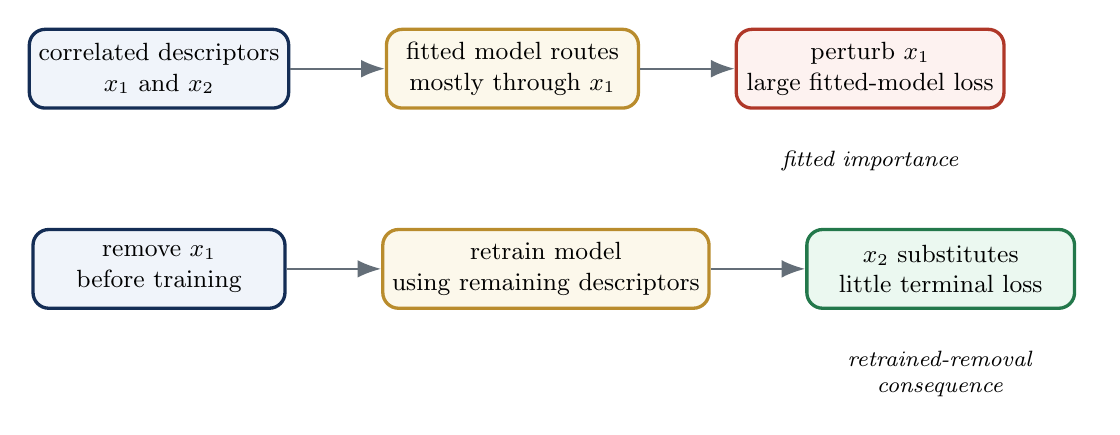
\begin{tikzpicture}[node distance=10mm and 12mm, every node/.style={ font=\small, align=center }, source/.style={ draw=geoBlue, very thick, rounded corners=2mm, fill=geoLight, minimum width=3.2cm, minimum height=1.0cm }, model/.style={ draw=geoGold, very thick, rounded corners=2mm, fill=geoGoldLight, minimum width=3.2cm, minimum height=1.0cm }, outcome/.style={ draw=geoGreen, very thick, rounded corners=2mm, fill=geoGreenLight, minimum width=3.4cm, minimum height=1.0cm }, fail/.style={ draw=geoRust, very thick, rounded corners=2mm, fill=geoRedLight, minimum width=3.4cm, minimum height=1.0cm }]
\node[source] (data1) {
    correlated descriptors\\
    $x_1$ and $x_2$
};
\node[
    model,
    right=of data1
] (fit1) {
    fitted model routes\\
    mostly through $x_1$
};
\node[
    fail,
    right=of fit1
] (perturb) {
    perturb $x_1$\\
    large fitted-model loss
};
\node[
    source,
    below=15mm of data1
] (data2) {
    remove $x_1$\\
    before training
};
\node[
    model,
    right=of data2
] (fit2) {
    retrain model\\
    using remaining descriptors
};
\node[
    outcome,
    right=of fit2
] (substitute) {
    $x_2$ substitutes\\
    little terminal loss
};
\draw[
    -{Latex[length=3mm]},
    thick,
    color=geoGrey
]
(data1) -- (fit1);
\draw[
    -{Latex[length=3mm]},
    thick,
    color=geoGrey
]
(fit1) -- (perturb);
\draw[
    -{Latex[length=3mm]},
    thick,
    color=geoGrey
]
(data2) -- (fit2);
\draw[
    -{Latex[length=3mm]},
    thick,
    color=geoGrey
]
(fit2) -- (substitute);
\node[
    draw=none,
    below=4mm of perturb,
    text width=3.6cm,
    font=\footnotesize\itshape
] {
    fitted importance
};
\node[
    draw=none,
    below=4mm of substitute,
    text width=3.6cm,
    font=\footnotesize\itshape
] {
    retrained-removal consequence
};
\end{tikzpicture}



\caption{Fitted importance and retrained-removal consequence answer different questions. A descriptor can be central to the information route used by one trained model while remaining replaceable when the model is trained again without it.}



\label{fig:importance-vs-necessity}



\end{figure}





Figure~\ref{fig:importance-vs-necessity} illustrates the central

distinction.



A highly ranked descriptor may be:



\begin{itemize}



\item

a physically meaningful variable;



\item

a strong fitted-model route;



\item

a stable correlate across several runs;



\item

yet still replaceable by other descriptors after retraining.



\end{itemize}



Conversely,

a quieter descriptor may appear less important in the fitted model but

prove difficult to replace when removed.



The brightest part of the explanation is not automatically the most

load-bearing part of the representation.





\begin{governingrule}



Importance describes a model's present information route.



Retrained removal tests what the modelling process can reconstruct when that

route is removed.



Authority cannot be inferred from either quantity alone.



\end{governingrule}





\section{Descriptor authority as bounded engineering permission}



Geatomica defines descriptor authority operationally.



For descriptor $j$,

target $t$

and evidenced domain $\mathcal{D}$,

authority is not a claim that the descriptor is universally true.



It is permission to use a specified relationship for a specified

purpose within a bounded domain.



A general representation is:



\begin{equation}
\label{eq:authority-general}
\mathcal{A}_{j,t,\mathcal{D}}
=
\Phi
\left(
P,
N,
T,
M,
S,
D,
R,
C
\right),
\end{equation}



where:



\begin{itemize}



\item

$P$ denotes predictive usefulness;



\item

$N$ denotes separation from negative controls;



\item

$T$ denotes transformation stability;



\item

$M$ denotes recurrence across model families;



\item

$S$ denotes recurrence across scale and population split;



\item

$D$ denotes source and domain admissibility;



\item

$R$ denotes replay and reproducibility evidence;



\item

$C$ denotes the claim or decision being requested.



\end{itemize}



Equation~\ref{eq:authority-general} is intentionally not reduced to a

single universal scalar.



Different engineering decisions place different demands on evidence.



A descriptor used to organise exploratory analysis does not require

the same evidence as one used to remove physical tests from a

qualification programme.



A relationship used to nominate a higher-fidelity calculation does

not require the same authority as one used to reject fabrication.



The claim is therefore part of the authority object.



Formally,

a permission can be written as:



\begin{equation}
\label{eq:permission}
\mathcal{P}
=
\left(
q,
\mathcal{D},
\mathcal{T},
\mathcal{E},
a
\right),
\end{equation}



where:



\begin{itemize}



\item

$q$ is the claim;



\item

$\mathcal{D}$ is the evidenced domain;



\item

$\mathcal{T}$ is the declared transformation family;



\item

$\mathcal{E}$ is the supporting evidence bundle;



\item

$a$ is the permitted action.



\end{itemize}



Examples of actions include:



\begin{itemize}



\item

retain for exploratory interpretation;



\item

nominate for a higher-fidelity calculation;



\item

use within a bounded screening model;



\item

request additional source resolution;



\item

hold interpretation;



\item

refuse downstream promotion.



\end{itemize}





\begin{engineeringconsequence}



Descriptor authority is meaningful only when attached to a decision.



Without a declared action,

``authority'' becomes an abstract label.



With a declared action,

it becomes testable:

the evidence either supports that permission or it does not.



\end{engineeringconsequence}





\section{The descriptor-response barcode}



A single ranking is too compressed to represent the evidence required

for authority.



Geatomica instead records a descriptor-response object.



For descriptor $j$,

target $t$

and material region $z$:



\begin{equation}
\label{eq:barcode}
\mathbf{b}_{j,t,z}
=
\left[
I,
\Delta_{\mathrm{noise}},
\Delta_{\mathrm{dropout}},
\Delta_{\mathrm{shuffle}},
\Delta_{\mathrm{removal}},
L_{\mathrm{scale}},
L_{\mathrm{split}},
R_{\mathrm{model}},
\Delta_{\mathrm{source}}
\right].
\end{equation}



The components are:



\begin{description}[leftmargin=3.6cm,style=nextline]



\item[$I$]

Baseline fitted importance under a declared model,

population

and explanation method.



\item[$\Delta_{\mathrm{noise}}$]

Change under controlled numerical disturbance.



\item[$\Delta_{\mathrm{dropout}}$]

Change when a declared fraction of eligible inputs is removed or made

missing.



\item[$\Delta_{\mathrm{shuffle}}$]

Loss after disrupting the association between one descriptor and the

other rows while retaining its marginal distribution.



\item[$\Delta_{\mathrm{removal}}$]

Performance consequence after the descriptor is removed and the model

is trained again.



\item[$L_{\mathrm{scale}}$]

Change across deterministic nested population sizes.



\item[$L_{\mathrm{split}}$]

Loss under increasingly difficult population-separation rules.



\item[$R_{\mathrm{model}}$]

Recurrence across model families and seeds.



\item[$\Delta_{\mathrm{source}}$]

Change across independently governed data environments.



\end{description}



The barcode does not assume that every component should move in the

same direction.



A descriptor can show:



\begin{itemize}



\item

high baseline importance;



\item

low noise sensitivity;



\item

large shuffle loss;



\item

small retrained-removal loss;



\item

strong recurrence across tree models;



\item

weak recurrence in a linear model;



\item

good within-source persistence;



\item

poor cross-source persistence.



\end{itemize}



That pattern is more informative than a terminal average.



It describes the shape of the evidence.





\begin{figure}[H]



\centering



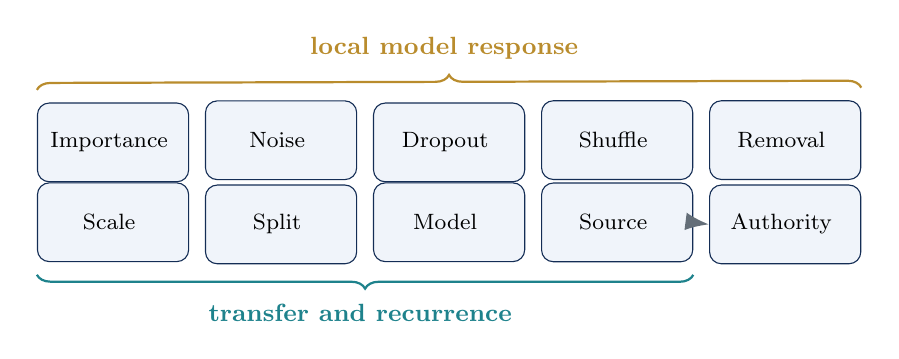
\begin{tikzpicture}[every node/.style={ font=\footnotesize, align=center }]
\matrix[
    matrix of nodes,
    nodes={
        draw=geoBlue,
        rounded corners=1.5mm,
        minimum width=1.92cm,
        minimum height=1.0cm,
        fill=geoLight
    },
    column sep=2mm
] (m) {
    Importance &
    Noise &
    Dropout &
    Shuffle &
    Removal \\
    Scale &
    Split &
    Model &
    Source &
    Authority \\
};
\draw[
    decorate,
    decoration={
        brace,
        amplitude=5pt
    },
    thick,
    color=geoGold
]
($(m-1-1.north west)+(0,0.16)$)
--
($(m-1-5.north east)+(0,0.16)$)
node[
    midway,
    above=7pt,
    draw=none,
    font=\small\bfseries,
    color=geoGold
] {
    local model response
};
\draw[
    decorate,
    decoration={
        brace,
        amplitude=5pt,
        mirror
    },
    thick,
    color=geoTeal
]
($(m-2-1.south west)+(0,-0.16)$)
--
($(m-2-4.south east)+(0,-0.16)$)
node[
    midway,
    below=7pt,
    draw=none,
    font=\small\bfseries,
    color=geoTeal
] {
    transfer and recurrence
};
\draw[
    -{Latex[length=3mm]},
    thick,
    color=geoGrey
]
(m-2-4.east)
--
(m-2-5.west);
\end{tikzpicture}



\caption{Conceptual descriptor-response barcode. The barcode keeps fitted response, disturbance response, retrained consequence and transfer evidence separate before a bounded authority decision is made.}



\label{fig:barcode}



\end{figure}





Descriptors can be compared in the response space using:



\begin{equation}
\label{eq:barcode-distance}
d(j,k)
=
\sqrt{
\left(
\mathbf{b}_{j}
-
\mathbf{b}_{k}
\right)^{\mathrm{T}}
\mathbf{W}
\left(
\mathbf{b}_{j}
-
\mathbf{b}_{k}
\right)
},
\end{equation}



where $\mathbf{W}$ is a declared weighting matrix.



The weighting must be frozen before terminal classification or

estimated through a separately governed procedure.



Unweighted analysis and sensitivity to $\mathbf{W}$ should be retained.



Otherwise,

the apparent geometry can be manufactured by convenient weighting.





\section{Bounded invariance rather than universal invariance}



The term \emph{invariance} can easily become stronger than finite

experiments permit.



No finite audit over a small family of transformations can establish

that a relation survives every possible admissible change.



The defensible object is bounded invariance under a declared

transformation family.



Let $\mathcal{T}^{*}$ be the finite set of transformations used by the

experiment.



For a quantity $q$:



\begin{equation}
\label{eq:bounded-invariance}
I_{\mathcal{T}^{*}}(q)
=
\Pr
\left[
q
\text{remains within its declared validity bounds under}
\tau
\in
\mathcal{T}^{*}
\right].
\end{equation}



The empirical programme estimates this bounded object.



It does not establish:



\begin{equation}
q
\text{is invariant under all conceivable transformations.}
\end{equation}



This produces an evidence ladder:



\begin{enumerate}



\item

\term{Observed}



The result appeared in one fitted configuration.



\item

\term{Repeated}



The result recurred across seeds or executions.



\item

\term{Boundedly persistent}



The result survived a declared transformation family.



\item

\term{Cross-source persistent}



The result recurred across provenance-separated source environments.



\item

\term{Mechanistically supported}



The relation was connected independently to physical intervention,

simulation,

measurement

or established domain theory.



\item

\term{Causal}



The relation survived an appropriate causal or interventional test.



\item

\term{Universal}



The relation is claimed to hold beyond the bounded evidence domain.



\end{enumerate}





\begin{figure}[H]



\centering



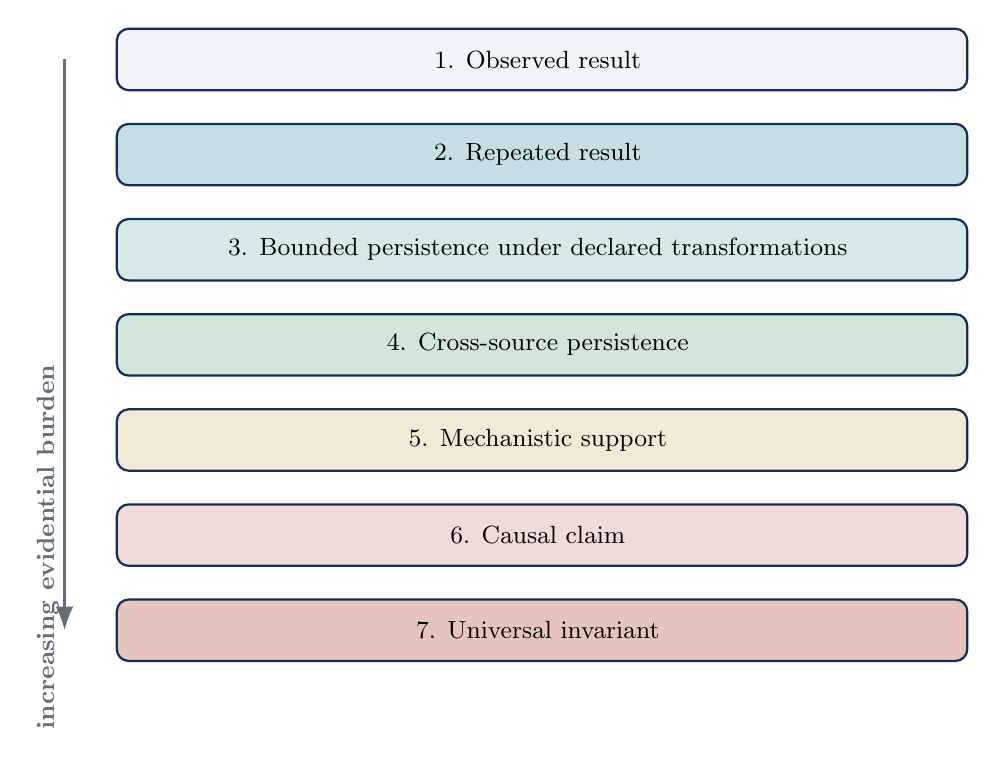
\begin{tikzpicture}[node distance=4mm, every node/.style={ font=\small, align=center }, level/.style={ rounded corners=1.5mm, minimum width=10.8cm, minimum height=0.78cm, draw=geoBlue, thick }]
\node[
    level,
    fill=geoLight
] (l1) {
    1. Observed result
};
\node[
    level,
    fill=geoLight!80!geoTeal,
    below=of l1
] (l2) {
    2. Repeated result
};
\node[
    level,
    fill=geoTeal!18,
    below=of l2
] (l3) {
    3. Bounded persistence under declared transformations
};
\node[
    level,
    fill=geoGreen!20,
    below=of l3
] (l4) {
    4. Cross-source persistence
};
\node[
    level,
    fill=geoGold!20,
    below=of l4
] (l5) {
    5. Mechanistic support
};
\node[
    level,
    fill=geoRust!18,
    below=of l5
] (l6) {
    6. Causal claim
};
\node[
    level,
    fill=geoRust!30,
    below=of l6
] (l7) {
    7. Universal invariant
};
\draw[
    -{Latex[length=3mm]},
    thick,
    color=geoGrey
]
($(l1.west)+(-0.65,0)$)
--
($(l7.west)+(-0.65,0)$)
node[
    midway,
    left=6pt,
    rotate=90,
    draw=none,
    font=\small\bfseries,
    color=geoGrey
] {
    increasing evidential burden
};
\end{tikzpicture}



\caption{Evidence ladder used to prevent bounded computational persistence from being promoted directly into causal or universal language. The present programme reaches different levels for different results.}



\label{fig:evidence-ladder}



\end{figure}





\begin{governingrule}



Every claim inherits the ceiling of its weakest required evidence

object.



A later interpretation cannot repair an earlier failed source,

viability

or replay gate.



\end{governingrule}





\section{The two named operational components}



\subsection{Governed Invariance Logic}



GIL is the audit logic applied to a declared scientific object.



Its function is to:



\begin{itemize}



\item

freeze the source,

target,

population

and descriptor conditions;



\item

declare the transformation family before terminal interpretation;



\item

apply controlled changes to model,

scale,

split,

input quality

and descriptor availability;



\item

compare valid models with paired negative controls;



\item

record persistence,

deformation,

substitution

and collapse;



\item

produce bounded evidence objects rather than one universal score.



\end{itemize}



GIL is not an autonomous truth engine.



It measures response under declared conditions.



The logic can be represented as:



\begin{equation}
\label{eq:gil-transform}
\left(
Q_{\mathrm{evidence}},
U,
\Pi_{\mathrm{audit}}
\right)
\xrightarrow{x_{\mathrm{GIL}}}
G_{\mathrm{authority}},
\end{equation}



where:



\begin{itemize}



\item

$Q_{\mathrm{evidence}}$ is the high-dimensional evidence state;



\item

$U$ defines source,

population,

representation

and experimental boundaries;



\item

$\Pi_{\mathrm{audit}}$ is the declared pressure or perturbation vector;



\item

$x_{\mathrm{GIL}}$ is the controlled transformation and measurement

route;



\item

$G_{\mathrm{authority}}$ is the lower-dimensional evidence geometry

used for bounded adjudication.



\end{itemize}



This is an operational research design,

not a claim that the geometry is a new physical ontology.





\subsection{Bounded candidate progression}

Candidate progression was organised using bounded multi-objective selection over
predictive error,
stability,
complexity,
compute
and declared risk.

The purpose was not to let one best-score criterion silently define scientific
progress.
Candidate options remained subject to the same frozen admission,
viability,
perturbation,
replay
and claim-boundary checks described elsewhere in this monograph.

This public evidence release reports the scientific questions,
measured outcomes
and bounded decision consequences needed to inspect the claims.
The reusable progression implementation,
advancement policy
and production orchestration are outside the public evidence release.
No candidate-selection mechanism was permitted to grant engineering authority.

\begin{reviewerquestion}[Why use bounded multi-objective progression?]

The experiment contains competing scientific and operational considerations.
A candidate that improves one score may become less stable,
more expensive,
more complex
or less capable of exposing a known failure mode.
Keeping those considerations visible prevents predictive improvement from
impersonating complete scientific progress.

\end{reviewerquestion}


\section{Supporting functions without architecture takeover}



Four further functions support the experiment.



They are described by what they do rather than introduced as additional

frameworks.



\begin{enumerate}



\item

\term{Visual evidence representation}



The response surface,

Pareto trade-offs,

descriptor zones,

source holds

and replay states must be visible to a human reviewer.



The visual layer does not change evidence.



It makes the current evidence geometry inspectable.



\item

\term{State memory and provenance}



The programme retains protocol identity,

source identity,

unit receipts,

checkpoints,

hashes,

terminal manifests,

accepted evidence

and rejected routes.



Narrative summaries are not treated as the authoritative source.



\item

\term{Operational governance}



The operating layer controls which module may execute,

what evidence may be promoted,

which state applies

and what claim ceiling remains in force.



\item

\term{Recovery control}



Long-running work is divided into complete scientific units.



Only units satisfying the expected-output contract are committed.



Interrupted work resumes from the last verified boundary.



\end{enumerate}



These functions become important later in the empirical programme.



They are not the scientific protagonist.



The scientific protagonist remains the materials relationship being

tested.





\section{Chapter conclusion}



Descriptor authority emerged because the experiments required a

stronger concept than fitted importance or repeated stability alone.



The framework preserves several distinctions:



\begin{itemize}



\item

importance versus necessity;



\item

prediction versus viability;



\item

repetition versus bounded persistence;



\item

cross-source recurrence versus matched-material transfer;



\item

numerical replay versus byte identity;



\item

evidence generation versus engineering permission.



\end{itemize}



The next chapter converts these distinctions into a frozen experimental

programme.



The central question is no longer only whether a descriptor looks

important.



It is whether its apparent role survives enough independent pressure

to support a bounded materials-engineering claim.







% ============================================================

% CHAPTER 3

% ============================================================



\chapter{Experimental Programme and Decision Logic}



\label{chap:experimental-design}





\section{Programme architecture}



The empirical programme was designed to expose disagreements that a

single benchmark score would hide.



The principal axes were:



\begin{itemize}



\item

target property;



\item

source environment;



\item

descriptor lane;



\item

population scale;



\item

split geometry;



\item

model family;



\item

random seed;



\item

negative control;



\item

input perturbation;



\item

descriptor removal;



\item

fresh versus replay execution.



\end{itemize}



The programme was not designed as an exhaustive search over every

possible material representation.



It was designed as a controlled first measurement of whether descriptor

interpretations persist across several scientifically meaningful

changes.



The experimental progression was:



\begin{equation}
\label{eq:programme-order}
\text{JARVIS}
\rightarrow
\text{Materials Project}
\rightarrow
\text{Matbench and Magpie}.
\end{equation}



Each stage inherited lessons from the earlier one,

but historical runs were not silently rewritten.



Corrections were introduced through named successor protocols.





\section{Target selection}



Four targets were selected to sample different positions in the

proposed materials chain.



\begin{table}[H]



\centering



\caption{Targets used in the four-property programme.}



\label{tab:targets}



\begin{tabularx}{\textwidth}{L{0.20\textwidth}
    L{0.19\textwidth}
    Y
    Y
}
\toprule
\textbf{Target}
&
\textbf{Unit}
&
\textbf{Physical role}
&
\textbf{Reason for inclusion}
\\
\midrule
Formation energy per atom
&
eV/atom
&
Energetic organisation and relative thermodynamic state.
&
Tests whether composition,
structure
and related property information reconstruct energetic organisation.
\\
\addlinespace
Band gap
&
eV
&
Electronic state and separation between occupied and unoccupied
electronic levels.
&
Provides an electronic target with known dependence on composition,
structure,
method
and material class.
\\
\addlinespace
Bulk modulus
&
GPa
&
Resistance to uniform volumetric deformation.
&
Tests recovery of a scalar mechanical response strongly connected to
bonding,
packing
and equation-of-state curvature.
\\
\addlinespace
Shear modulus
&
GPa
&
Resistance to shape change at approximately constant volume.
&
Provides a more directionally sensitive mechanical target expected to
be less accessible through coarse tabular descriptors.
\\
\bottomrule
\end{tabularx}



\end{table}





Formation energy and band gap used the largest available coherent

populations.



The elastic targets were limited to records exposing the relevant

source quantities.



No target was assumed to be automatically admissible because the field

was present.





\section{Descriptor lanes}



Two principal lanes were used.



\subsection{Common descriptor lane}



The common lane provided a shared comparison substrate across all four

targets.



It included a conservative set of descriptors such as:



\begin{itemize}



\item

density;



\item

volume per atom;



\item

site count;



\item

total magnetisation;



\item

lattice lengths;



\item

lattice angles;



\item

crystal system.



\end{itemize}



The purpose of the common lane was not to maximise predictive

performance.



It allowed the same broad representation to be compared across

energetic,

electronic

and elastic targets.





\subsection{Target-specific non-leaking lane}



The target-specific lane added related properties only where a frozen

exclusion register permitted them.



Examples included energetic or electronic information when not

directly equivalent to the target.



The lane excluded:



\begin{itemize}



\item

the target itself;



\item

direct target siblings;



\item

post-target labels;



\item

derived quantities that reconstructed the target trivially;



\item

identifiers or source artefacts;



\item

features listed in the leakage register.



\end{itemize}



The label \emph{target-specific} does not mean causal.



It means the descriptor set contains additional information relevant

to that target under a frozen non-leakage contract.





\begin{table}[H]



\centering



\caption{Purpose and boundary of the two descriptor lanes.}



\label{tab:descriptor-lanes}



\begin{tabularx}{\textwidth}{L{0.19\textwidth}
    Y
    Y
}
\toprule
\textbf{Lane}
&
\textbf{Purpose}
&
\textbf{Boundary}
\\
\midrule
Common
&
Compare targets under a shared,
conservative tabular representation.
&
May omit useful target-specific information;
does not represent the strongest possible predictor.
\\
\addlinespace
Target-specific
&
Test whether admissible related properties improve prediction and
change descriptor response.
&
Measures information transfer,
not causality;
every target requires a separate exclusion register.
\\
\bottomrule
\end{tabularx}



\end{table}





\section{Population scales}



Deterministic nested cohorts were constructed at:



\begin{equation}
n
\in
\left\{
2{,}000,
5{,}000,
10{,}000,
n_{\mathrm{full}}
\right\}.
\end{equation}



The smaller cohorts were nested within the larger populations.



This allows scale response to be interpreted without replacing the

underlying population arbitrarily at each size.



The scale experiment asks:



\begin{itemize}



\item

Does predictive signal improve as more records become available?



\item

Does descriptor ordering stabilise with scale?



\item

Do some descriptors appear only at small or large population sizes?



\item

Does performance convergence coincide with explanation convergence?



\end{itemize}



The final question is especially important.



A model can improve steadily with more data while the apparent

descriptor account remains conditional on model or split.





\section{Population splits}



Three split views were used.



\subsection{Row-random split}



Rows were divided randomly under a fixed seed and test fraction.



This is the least demanding view.



It primarily tests interpolation across records drawn from a similar

overall population.





\subsection{Reduced-composition group split}



Records sharing the same reduced composition were assigned to the same

group.



This prevents identical reduced formulae from appearing on both sides

of the split.



It asks whether the model transfers to unseen compositions rather than

only unseen records.





\subsection{Chemical-system group split}



Records sharing the same element set were assigned to the same group.



This is a harder population shift.



It asks whether the learned relation persists when complete element

combinations are withheld.





\begin{figure}[H]



\centering



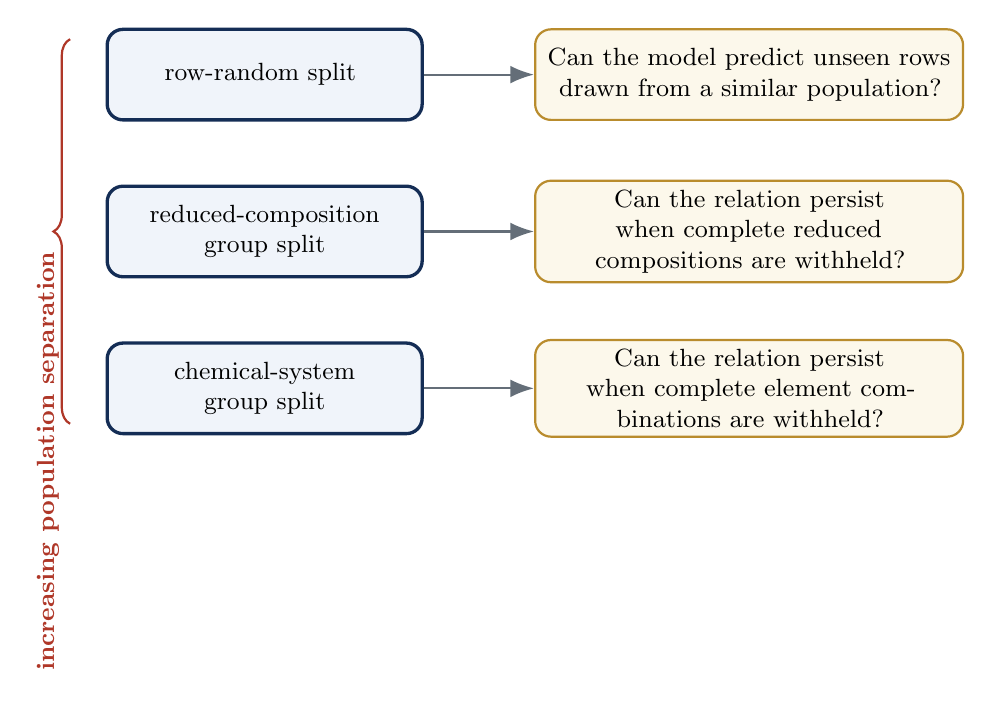
\begin{tikzpicture}[node distance=8mm and 8mm, every node/.style={ font=\small, align=center }, split/.style={ draw=geoBlue, very thick, rounded corners=2mm, fill=geoLight, minimum width=4.0cm, minimum height=1.15cm }, question/.style={ draw=geoGold, thick, rounded corners=2mm, fill=geoGoldLight, text width=5.2cm, minimum height=1.15cm }]
\node[split] (random) {
    row-random split
};
\node[
    split,
    below=of random
] (composition) {
    reduced-composition\\
    group split
};
\node[
    split,
    below=of composition
] (chemistry) {
    chemical-system\\
    group split
};
\node[
    question,
    right=14mm of random
] (q1) {
    Can the model predict unseen rows drawn from a similar population?
};
\node[
    question,
    right=14mm of composition
] (q2) {
    Can the relation persist when complete reduced compositions are
    withheld?
};
\node[
    question,
    right=14mm of chemistry
] (q3) {
    Can the relation persist when complete element combinations are
    withheld?
};
\draw[
    -{Latex[length=3mm]},
    thick,
    color=geoGrey
]
(random) -- (q1);
\draw[
    -{Latex[length=3mm]},
    thick,
    color=geoGrey
]
(composition) -- (q2);
\draw[
    -{Latex[length=3mm]},
    thick,
    color=geoGrey
]
(chemistry) -- (q3);
\draw[
    decorate,
    decoration={
        brace,
        amplitude=6pt,
        mirror
    },
    thick,
    color=geoRust
]
($(random.west)+(-0.45,0.45)$)
--
($(chemistry.west)+(-0.45,-0.45)$)
node[
    midway,
    left=8pt,
    rotate=90,
    draw=none,
    font=\small\bfseries,
    color=geoRust
] {
    increasing population separation
};
\end{tikzpicture}



\caption{The three split views represent different scientific claims. Performance under row-random separation cannot be treated as evidence of unseen-composition or unseen-chemical-system transfer.}



\label{fig:split-claims}



\end{figure}





\begin{governingrule}



The split is part of the claim.



Prediction of unseen rows,

unseen compositions

and unseen element systems are not interchangeable forms of

generalisation.



\end{governingrule}





\section{Model families}



The first two source programmes used four model families:



\begin{enumerate}



\item

\term{Ridge regression}



A regularised linear baseline.



\item

\term{Random Forest}



A nonlinear bagged tree ensemble.



\item

\term{Extra Trees}



A highly randomised nonlinear tree ensemble.



\item

\term{HistGradientBoosting}



A sequential nonlinear boosting model.



\end{enumerate}



The model set was selected to compare:



\begin{itemize}



\item

linear and nonlinear information routing;



\item

bagged and boosted ensembles;



\item

different sensitivity to feature scaling,

interactions

and threshold structure;



\item

different explanation behaviours under permutation,

shuffle

and removal.



\end{itemize}



The aim was not to identify one universally best model.



It was to determine whether conclusions survived materially different

learners.



A later multilayer perceptron added a distributed nonlinear learner in

the Matbench/Magpie stage.





\section{Preprocessing and leakage control}



All preprocessing was fitted using the training population only.



Numeric descriptors were:



\begin{itemize}



\item

median-imputed from the training set;



\item

standardised where required by the model family;



\item

kept in a floating-point working frame during dropout so that missing

values could be represented without mutating integer source columns.



\end{itemize}



Categorical descriptors such as crystal system were:



\begin{itemize}



\item

most-frequent imputed using the training set;



\item

one-hot encoded;



\item

configured to ignore categories unseen during training.



\end{itemize}



The leakage scan included:



\begin{itemize}



\item

explicit forbidden columns;



\item

identifier-like names;



\item

post-target fields;



\item

direct target derivatives;



\item

suspiciously perfect target correlations;



\item

source-specific leakage routes.



\end{itemize}



All transformations used during fitting were contained inside the

training pipeline.





\section{Negative controls}



Each full-scale valid model cell was paired with target-permutation

nulls.



The training target was shuffled while retaining:



\begin{itemize}



\item

the source cohort;



\item

the split;



\item

the descriptor matrix;



\item

the preprocessing route;



\item

the model family;



\item

the seed context.



\end{itemize}



This produced a paired null score:



\begin{equation}
\Rnull.
\end{equation}



The valid-minus-null separation was:



\begin{equation}
\label{eq:null-separation}
S
=
\Rvalid
-
\Rnull.
\end{equation}



A positive $S$ indicates that the valid target carries more learnable

structure than the paired shuffled target under that cell.



It does not establish that the valid model is useful.





\section{The two-door model-viability rule}



The Materials Project experiment exposed a defect in the original

aggregation logic.



A model could satisfy:



\begin{equation}
S>0
\end{equation}



while still satisfying:



\begin{equation}
R^2<0.
\end{equation}



The model had beaten the deliberately weakened comparator while

remaining worse than predicting the mean.



The corrected rule requires:



\begin{equation}
\label{eq:two-door}
\text{viable support}
\iff
\left(
R^2
>
\tau_{\mathrm{absolute}}
\right)
\land
\left(
S
>
\tau_{\mathrm{separation}}
\right).
\end{equation}



For the baseline exposed in this monograph:



\begin{equation}
\tau_{\mathrm{absolute}}
=
0,
\qquad
\tau_{\mathrm{separation}}
=
0.
\end{equation}





\begin{table}[H]



\centering



\caption{Two-door model-viability decisions.}



\label{tab:two-door}



\begin{tabularx}{\textwidth}{L{0.23\textwidth}
    C{0.13\textwidth}
    C{0.13\textwidth}
    Y
}
\toprule
\textbf{State}
&
\textbf{$R^2>0$}
&
\textbf{$S>0$}
&
\textbf{Bounded decision}
\\
\midrule
Absolute and relative pass
&
Pass
&
Pass
&
Candidate may be nominated for bounded interpretation.
\\
\addlinespace
Relative-only pass
&
Fail
&
Pass
&
\hold{}.
Signal may exist,
but the model is not absolutely viable.
\\
\addlinespace
Absolute-only pass
&
Pass
&
Fail
&
\hold{}.
The model has not separated from the paired null under the declared
control.
\\
\addlinespace
Both fail
&
Fail
&
Fail
&
\refuse{} predictive interpretation.
\\
\bottomrule
\end{tabularx}



\end{table}





\begin{engineeringconsequence}



A broken thermometer may outperform a random-number generator while

remaining a broken thermometer.



Relative improvement is evidence.



It is not viability.



\end{engineeringconsequence}





\section{Perturbation routes}



The declared perturbation family included:



\subsection{Numerical noise}



Gaussian noise was applied to eligible numeric descriptors at a

declared fraction of each descriptor's observed standard deviation.



The primary JARVIS route used 2\% noise.



This tests local numerical sensitivity.



It is not a model of physical ageing,

oxidation,

fatigue

or measurement degradation.





\subsection{Descriptor dropout}



A declared fraction of eligible numeric cells was replaced with

missing values.



The primary full-scale route used 10\% independent cell dropout.



This tests tolerance to incomplete descriptor availability.





\subsection{Within-feature shuffle}



One descriptor was shuffled across rows.



Its marginal distribution was retained,

but its association with the target and other row-level information

was disrupted.





\subsection{Permutation importance}



Prediction loss was measured after feature permutation in the fitted

model.





\subsection{Complete retrained removal}



A descriptor or descriptor group was removed before fitting.



The preprocessing and model were reconstructed using the remaining

representation.



This measures substitutability within the available feature space.





\section{Metrics and aggregation}

The executable routes used scikit-learn's \texttt{r2\_score(y\_true,y\_pred)}:
\[
R^2=1-\frac{\sum_i(y_i-\hat y_i)^2}{\sum_i(y_i-\bar y_{\mathrm{eval}})^2},
\]
where $\bar y_{\mathrm{eval}}$ is the mean of the evaluated held-out targets. Earlier
training-mean wording was a manuscript error. Positive $R^2$ is the minimal
demonstrated absolute boundary against this constant reference in the present
failure-analysis route, not a universal engineering threshold. MAE, RMSE, null gaps,
fold recurrence and declared perturbation effects remain separate evidence objects.

Aggregation rules were frozen before result inspection. Split views are reported
separately where the protocol requires separate adjudication.

\section{Replay contracts}



Replay was adjudicated through separate contracts.



\begin{enumerate}



\item

\term{Plan identity}



The same ordered scientific-unit plan must be executed.



\item

\term{Source and configuration identity}



Dataset,

code,

configuration,

dependency

and preprocessing identities must match the frozen contract.



\item

\term{Schema identity}



Expected files,

rows,

columns

and identifiers must be present.



\item

\term{Semantic identity}



Corresponding values must refer to the same scientific objects.



\item

\term{Numerical equivalence}



Compared numeric values must remain within the frozen tolerance.



\item

\term{Raw-byte identity}



Corresponding files must be byte-identical.



\end{enumerate}



The principal numerical tolerance was:



\begin{equation}
\left|
x_{\mathrm{fresh}}
-
x_{\mathrm{replay}}
\right|
\leq
10^{-10}.
\end{equation}



Byte identity was judged separately.



A numerically equivalent result was not described as byte-identical

when the byte contract failed.





\section{Atomic scientific units and recovery}



The execution controller used:



\begin{itemize}



\item

a canonical ordered unit plan;



\item

single-writer locking;



\item

append-only journals;



\item

atomic unit commits;



\item

expected-output contracts;



\item

hash verification;



\item

incomplete-unit rejection;



\item

resume under the same execution identity;



\item

terminal full-disk verification.



\end{itemize}



\textbf{Scientific unit:} one complete, independently committable part of the declared experiment. It may contain one estimator fit, several fits, a control set, or a solver/scenario calculation. A complete scientific unit was the smallest accepted restart boundary.



An interrupted staging unit was not promoted merely because some files

existed.



This distinction protects the scientific record from partial

completion being mistaken for accepted evidence.





\section{Chapter conclusion}



The experimental design treats source,

model,

split,

scale,

perturbation

and replay as parts of the scientific object.



It does not ask only whether prediction survives.



It asks which parts of the explanatory account survive,

which parts are reconstructed through alternatives,

and which claims become inadmissible.



The first full application of this design was the JARVIS-DFT

programme.







% ============================================================

% CHAPTER 4

% ============================================================



\chapter[JARVIS-DFT: The First Complete Audit]{JARVIS-DFT:\\ The First Complete Audit}

\begin{center}
\fbox{\begin{minipage}{0.91\textwidth}
\textbf{Question.} Can compact descriptors carry useful signal across targets, models, population splits, scale, and perturbation?\\
\textbf{Comparison.} Four targets were tested across common and target-specific descriptors, four classical models, three seeds, three split strategies, four scales, perturbations, removals, and paired target-permutation nulls.\\
\textbf{Result.} Useful but target-, model-, and population-dependent signal was observed; the 48-unit replay was numerically equivalent across 28,248 cells (maximum difference approximately $1.07	imes10^{-14}$).\\
\textbf{Decision.} Retain JARVIS as the coherent baseline and as evidence that null separation and useful prediction can coexist.\\
\textbf{Boundary.} Local measured and same-environment replayed evidence; not external validation or physical mechanism proof.
\end{minipage}}
\end{center}




\label{chap:jarvis}





\section{Role of the JARVIS stage}



JARVIS-DFT supplied the first complete execution of the four-target

programme.



Its scientific role was to establish:



\begin{itemize}



\item

whether sufficient predictive carrier signal existed across energetic,

electronic

and elastic targets;



\item

whether target-specific information improved performance without

leakage;



\item

whether model,

scale

and population split changed the apparent descriptor account;



\item

whether controlled noise and dropout exposed different forms of

fragility;



\item

whether the complete scientific programme could be independently

replayed under a frozen contract.



\end{itemize}



The JARVIS stage was not designed to prove cross-source transfer.



It established the first bounded evidence surface against which the

Materials Project and Matbench stages could later be compared.





\section{Source census and cohorts}



The processed JARVIS-DFT \texttt{dft\_3d} source census contained:



\begin{equation}
75{,}993
\end{equation}



calculated records.



Formation-energy and band-gap maximum-coverage cohorts retained up to

the full source census.



The four-property common and elastic cohort contained:



\begin{equation}
23{,}824
\end{equation}



records with the required target availability.



The source snapshot retained negative elastic values rather than

silently removing them.



The processed population included:



\begin{itemize}



\item

277 negative bulk-modulus values;



\item

1,951 negative shear-modulus values.



\end{itemize}



These values were retained in the original execution.



A separate sensitivity protocol was required before any later decision

to exclude or classify them.



The JARVIS records are calculated database objects.



They are not independently measured specimens.





\begin{table}[H]



\centering



\caption{JARVIS source and execution summary.}



\label{tab:jarvis-summary}



\begin{tabularx}{\textwidth}{L{0.30\textwidth}
    L{0.20\textwidth}
    Y
}
\toprule
\textbf{Object}
&
\textbf{Observed value}
&
\textbf{Meaning}
\\
\midrule
Processed source census
&
75,993 records
&
Full local JARVIS-DFT census used by the source freeze.
\\
\addlinespace
Four-property common cohort
&
23,824 records
&
Population exposing formation energy,
band gap,
bulk modulus
and shear modulus under the frozen membership rules.
\\
\addlinespace
Fresh scientific units
&
48/48
&
Complete and terminally sealed.
\\
\addlinespace
Replay scientific units
&
48/48
&
Complete and independently sealed.
\\
\addlinespace
Model-result rows
&
1,728
&
Baseline,
scale,
model,
seed
and split results.
\\
\addlinespace
Descriptor-response rows
&
1,860
&
Importance,
disturbance
and removal responses.
\\
\addlinespace
Fresh wall time
&
9.93 h
&
Eight-worker workstation-scale execution.
\\
\bottomrule
\end{tabularx}



\end{table}





\section{Full-scale predictive carrier signal}



Extra Trees produced the strongest full-scale mean performance in each

target/lane summary.



These values establish a usable carrier signal for the audit.



They do not establish state-of-the-art prediction.



\begin{table}[H]



\centering



\caption{Full-scale JARVIS Extra Trees performance. Means and standard deviations are calculated over the declared seeds and split views.}



\label{tab:jarvis-extra-trees}



\begin{tabular}{l l S[table-format=1.3] S[table-format=1.3] S[table-format=2.3] S[table-format=1.3]}
\toprule
\textbf{Target}
&
\textbf{Lane}
&
{\textbf{Mean $R^2$}}
&
{\textbf{SD}}
&
{\textbf{MAE}}
&
{\textbf{$R^2$--null}}
\\
\midrule
Formation energy
&
Common
&
0.703
&
0.021
&
0.387
&
0.822
\\
Formation energy
&
Target-specific
&
0.759
&
0.016
&
0.349
&
0.876
\\
Band gap
&
Common
&
0.593
&
0.044
&
0.418
&
0.704
\\
Band gap
&
Target-specific
&
0.759
&
0.041
&
0.313
&
0.849
\\
Bulk modulus
&
Common
&
0.759
&
0.017
&
20.095
&
0.883
\\
Bulk modulus
&
Target-specific
&
0.780
&
0.017
&
18.850
&
0.890
\\
Shear modulus
&
Common
&
0.607
&
0.040
&
15.102
&
0.730
\\
Shear modulus
&
Target-specific
&
0.679
&
0.041
&
13.332
&
0.786
\\
\bottomrule
\end{tabular}



\end{table}





\begin{figure}[H]



\centering



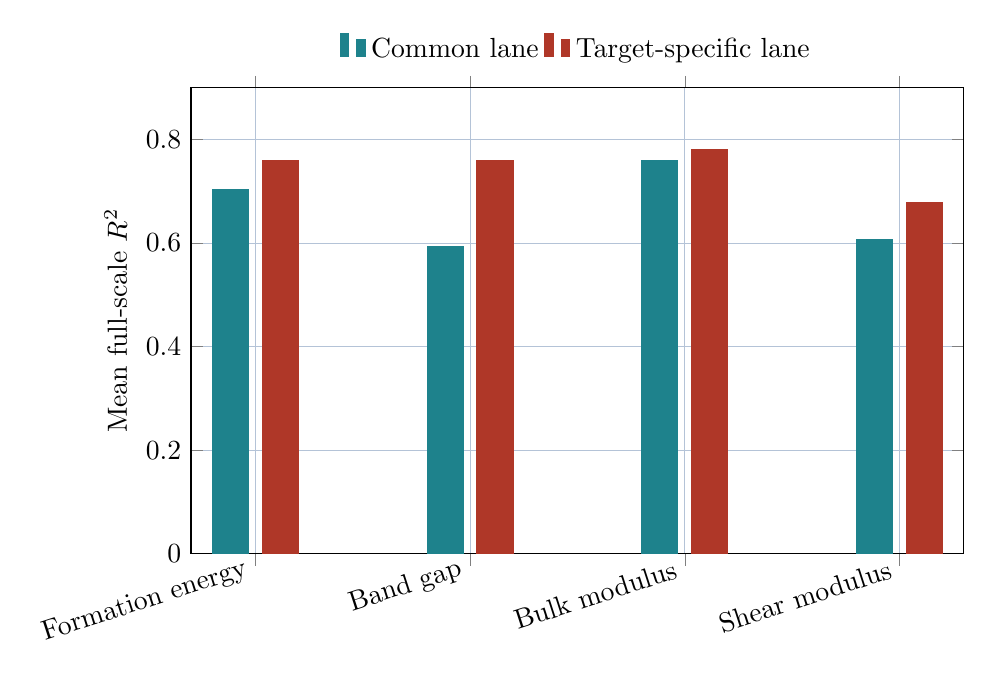
\begin{tikzpicture}
\begin{axis}[width=0.94\textwidth, height=7.5cm, ybar=5pt, bar width=13pt, ymin=0, ymax=0.90, ylabel={Mean full-scale $R^2$}, symbolic x coords={ Formation energy, Band gap, Bulk modulus, Shear modulus }, xtick=data, x tick label style={ rotate=18, anchor=east }, legend style={ at={(0.5,1.03)}, anchor=south, legend columns=2, draw=none }, grid=major, grid style={ draw=geoMid, line width=0.25pt }]
\addplot[
    fill=geoTeal,
    draw=geoTeal
]
coordinates {
    ({Formation energy},0.703)
    ({Band gap},0.593)
    ({Bulk modulus},0.759)
    ({Shear modulus},0.607)
};
\addplot[
    fill=geoRust,
    draw=geoRust
]
coordinates {
    ({Formation energy},0.759)
    ({Band gap},0.759)
    ({Bulk modulus},0.780)
    ({Shear modulus},0.679)
};
\legend{
    Common lane,
    Target-specific lane
}
\end{axis}
\end{tikzpicture}



\caption{Full-scale JARVIS Extra Trees carrier signal by target and descriptor lane. Target-specific information improved all four targets, with the largest absolute gain for band gap.}



\label{fig:jarvis-fullscale}



\end{figure}





Three principal patterns appear.



First,

bulk modulus was more accessible than shear modulus under the common

tabular route.



This is physically plausible.



Bulk response is a volumetric aggregate that can be strongly connected

to bonding strength,

density

and packing.



Shear response is more sensitive to directional bonding,

symmetry,

slip geometry

and anisotropy,

much of which is compressed or absent in coarse tabular descriptors.



This interpretation remains provisional.



The experiment supports target-dependent recoverability.



It does not prove the underlying mechanism.



Second,

target-specific information improved all four targets.



The largest gain was observed for band gap:



\begin{equation}
0.593
\rightarrow
0.759.
\end{equation}



This indicates that the common lane omitted substantial

target-relevant information.



Third,

every full-scale valid cell with a paired null showed positive

valid-minus-null separation.



The JARVIS routes therefore contained meaningful non-null signal under

the tested conditions.






\begin{figure}[H]
\centering
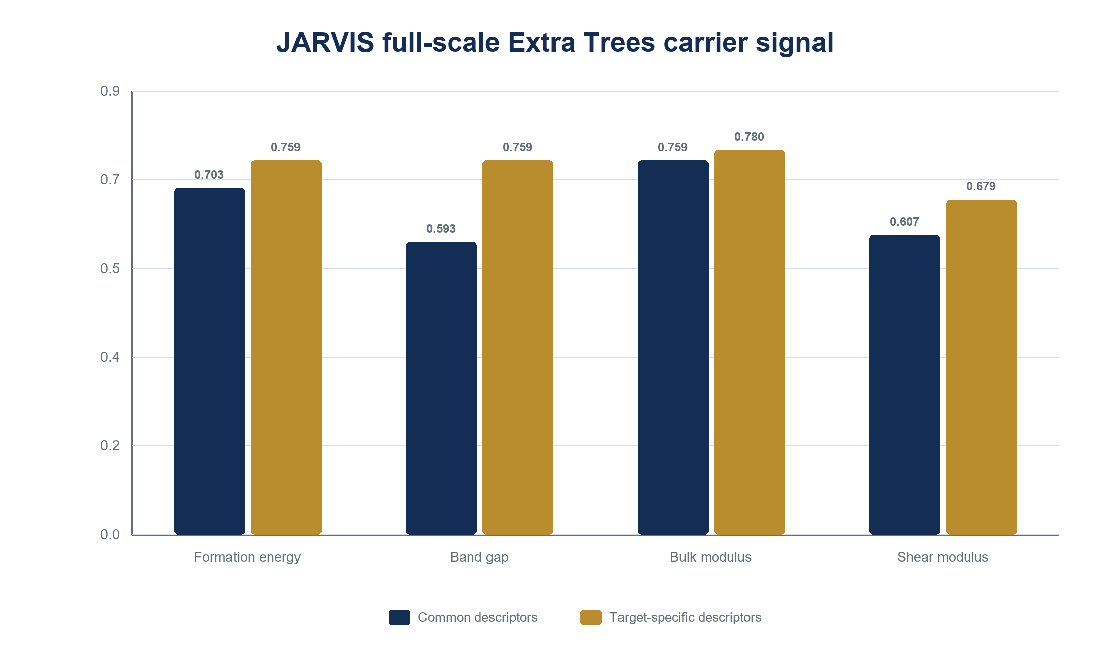
\includegraphics[width=0.92\textwidth]{figures/jarvis_carrier_signal.pdf}
\caption{\textbf{HISTORICAL REPORT BOUND.} Full-scale Extra Trees carrier signal for the common and target-specific JARVIS descriptor lanes. The plotted values are reproduced from the claim ledger whose rows bind the accepted estate-audit report hash.}
\label{fig:jarvis-carrier-evidence-edition}
\end{figure}

\section{Scale convergence}



Median $R^2$ increased from 2,000 rows to the full admissible

population for all eight target/lane aggregates.



Common-lane median values increased approximately as follows:



\begin{align}
\text{formation energy:}
\qquad
0.498
&\rightarrow
0.640,
\\
\text{band gap:}
\qquad
0.355
&\rightarrow
0.546,
\\
\text{bulk modulus:}
\qquad
0.647
&\rightarrow
0.742,
\\
\text{shear modulus:}
\qquad
0.421
&\rightarrow
0.574.
\end{align}



Larger populations improved prediction.



They did not eliminate model or split dependence.





\begin{figure}[H]



\centering



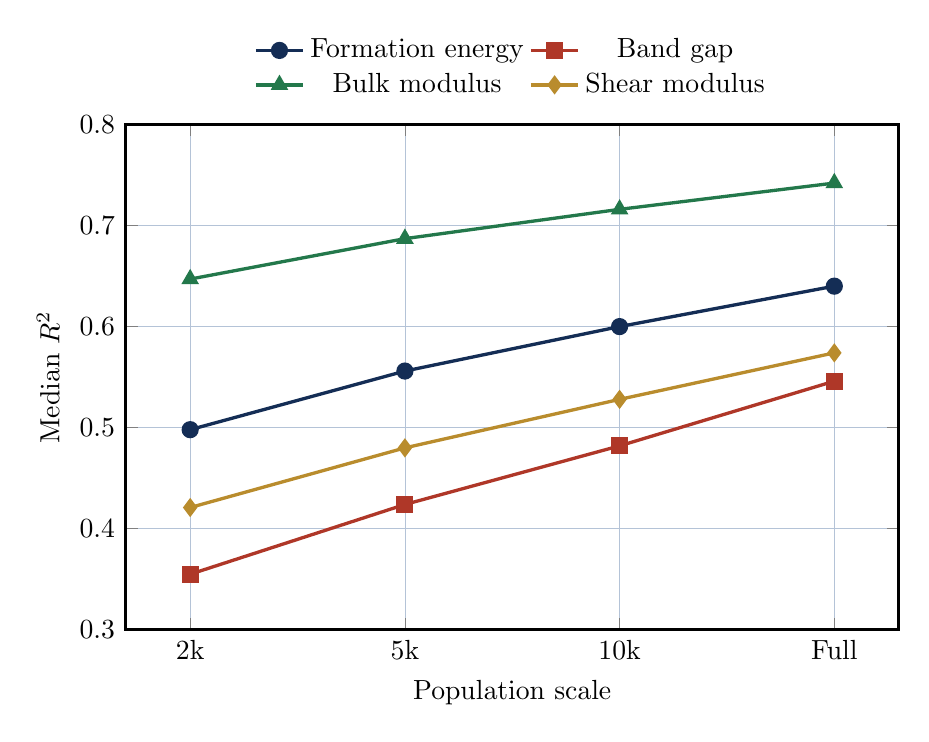
\begin{tikzpicture}
\begin{axis}[width=0.94\textwidth, height=8cm, xlabel={Population scale}, ylabel={Median $R^2$}, symbolic x coords={ 2k, 5k, 10k, Full }, xtick=data, ymin=0.30, ymax=0.80, legend style={ at={(0.5,1.03)}, anchor=south, legend columns=2, draw=none }, grid=major, grid style={ draw=geoMid, line width=0.25pt }, line width=1.2pt, mark size=2.5pt]
\addplot[
    color=geoBlue,
    mark=*
]
coordinates {
    (2k,0.498)
    (5k,0.556)
    (10k,0.600)
    (Full,0.640)
};
\addplot[
    color=geoRust,
    mark=square*
]
coordinates {
    (2k,0.355)
    (5k,0.424)
    (10k,0.482)
    (Full,0.546)
};
\addplot[
    color=geoGreen,
    mark=triangle*
]
coordinates {
    (2k,0.647)
    (5k,0.687)
    (10k,0.716)
    (Full,0.742)
};
\addplot[
    color=geoGold,
    mark=diamond*
]
coordinates {
    (2k,0.421)
    (5k,0.480)
    (10k,0.528)
    (Full,0.574)
};
\legend{
    Formation energy,
    Band gap,
    Bulk modulus,
    Shear modulus
}
\end{axis}
\end{tikzpicture}



\caption{Common-lane scale response in JARVIS across 2k, 5k, 10k and full-scale cohorts ($N=23{,}824$). All four targets show monotonic performance scaling as training population expands, with the highest relative sensitivity observed for band gap.}



\label{fig:jarvis-scale}
\end{figure}

The scale result supports two conclusions.



First,

the signal was not confined to one small pilot cohort.



Second,

performance convergence did not settle the descriptor account.



The larger populations still produced material differences across

models and population splits.





\section{Population-split dependence}



Grouped splits generally reduced target-specific performance relative

to row-random separation.



The hardest grouped view depended on the target.



Chemical-system separation was most costly for:



\begin{itemize}



\item

formation energy;



\item

band gap.



\end{itemize}



Reduced-composition grouping was slightly more costly for:



\begin{itemize}



\item

bulk modulus;



\item

shear modulus.



\end{itemize}



This prevents a universal ordering in which one split is always

hardest.



The result is target-dependent.





\begin{figure}[H]



\centering



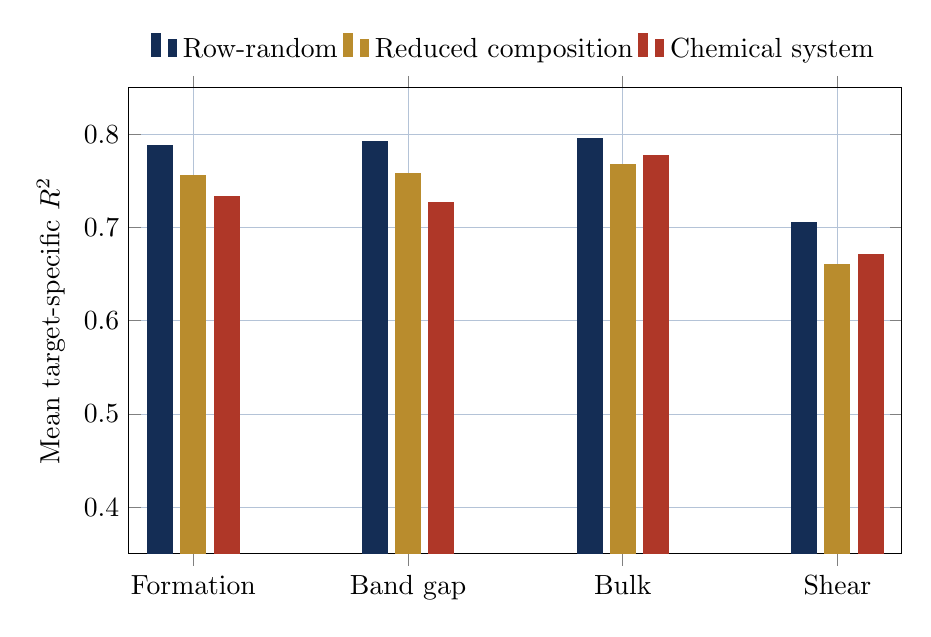
\begin{tikzpicture}
\begin{axis}[width=0.94\textwidth, height=7.5cm, ybar=3pt, bar width=9pt, ymin=0.35, ymax=0.85, ylabel={Mean target-specific $R^2$}, symbolic x coords={ Formation, Band gap, Bulk, Shear }, xtick=data, legend style={ at={(0.5,1.03)}, anchor=south, legend columns=3, draw=none }, grid=major, grid style={ draw=geoMid, line width=0.25pt }]
\addplot[
    fill=geoBlue,
    draw=geoBlue
]
coordinates {
    (Formation,0.788)
    ({Band gap},0.792)
    (Bulk,0.795)
    (Shear,0.705)
};
\addplot[
    fill=geoGold,
    draw=geoGold
]
coordinates {
    (Formation,0.756)
    ({Band gap},0.758)
    (Bulk,0.768)
    (Shear,0.660)
};
\addplot[
    fill=geoRust,
    draw=geoRust
]
coordinates {
    (Formation,0.733)
    ({Band gap},0.727)
    (Bulk,0.777)
    (Shear,0.671)
};
\legend{
    Row-random,
    Reduced composition,
    Chemical system
}
\end{axis}
\end{tikzpicture}



\caption{Target-specific split dependence in JARVIS across row-random, reduced-composition and chemical-system splits. Grouped splits reduce mean predictive performance relative to row-random splits for all four targets. Chemical-system separation is harder for formation energy and band gap; reduced-composition grouping is slightly harder for bulk and shear modulus.}



\label{fig:jarvis-splits}
\end{figure}

The grouped-split result has a direct engineering meaning.



A model that performs well when chemically related records occur on

both sides of the split should not automatically guide decisions about

unseen chemical systems.



The population boundary must follow the intended use.





\section{Model-family dependence}



Ridge remained materially below the nonlinear ensembles.



In the common lane,

full-scale mean $R^2$ values were:



\begin{table}[H]



\centering



\caption{Common-lane Ridge and Extra Trees comparison.}



\label{tab:ridge-extra}



\begin{tabular}{l S[table-format=1.3] S[table-format=1.3] S[table-format=1.3]}
\toprule
\textbf{Target}
&
{\textbf{Ridge}}
&
{\textbf{Extra Trees}}
&
{\textbf{Difference}}
\\
\midrule
Formation energy
&
0.244
&
0.703
&
0.459
\\
Band gap
&
0.247
&
0.593
&
0.346
\\
Bulk modulus
&
0.476
&
0.759
&
0.283
\\
Shear modulus
&
0.256
&
0.607
&
0.351
\\
\bottomrule
\end{tabular}



\end{table}





The difference suggests that the recoverable information is

substantially nonlinear and interaction-dependent.



It does not mean that tree structure is the physical mechanism.



Tree ensembles can also exploit:



\begin{itemize}



\item

correlated proxies;



\item

local population structure;



\item

threshold artefacts;



\item

redundancy;



\item

source-specific quirks.



\end{itemize}



Their strong performance strengthens the case for cross-model

descriptor auditing.



It does not grant the tree model's explanation privileged physical

authority.





\begin{reviewerquestion}[Why retain a weak linear model?]



The purpose of Ridge is not to compete for the highest score.



It provides a deliberately different information-routing regime.



When linear and nonlinear learners disagree,

that disagreement is evidence about the conditional nature of the

descriptor account.



Removing the weaker model would make the reported explanation appear

more coherent by construction.



\end{reviewerquestion}





\section{Noise and dropout response}



At full scale,

2\% numerical noise produced Extra Trees mean $R^2$ losses of

approximately:



\begin{equation}
0.002
\text{to}
0.037.
\end{equation}



Ten-percent descriptor dropout produced larger losses of:



\begin{equation}
0.066
\text{to}
0.106.
\end{equation}



The two disturbances answer different questions.



Small numerical noise tests local smoothness around the observed

descriptor values.



Dropout tests dependence on descriptor availability.



A model can be robust to small numerical disturbance while depending

strongly on complete descriptor coverage.





\begin{figure}[H]



\centering



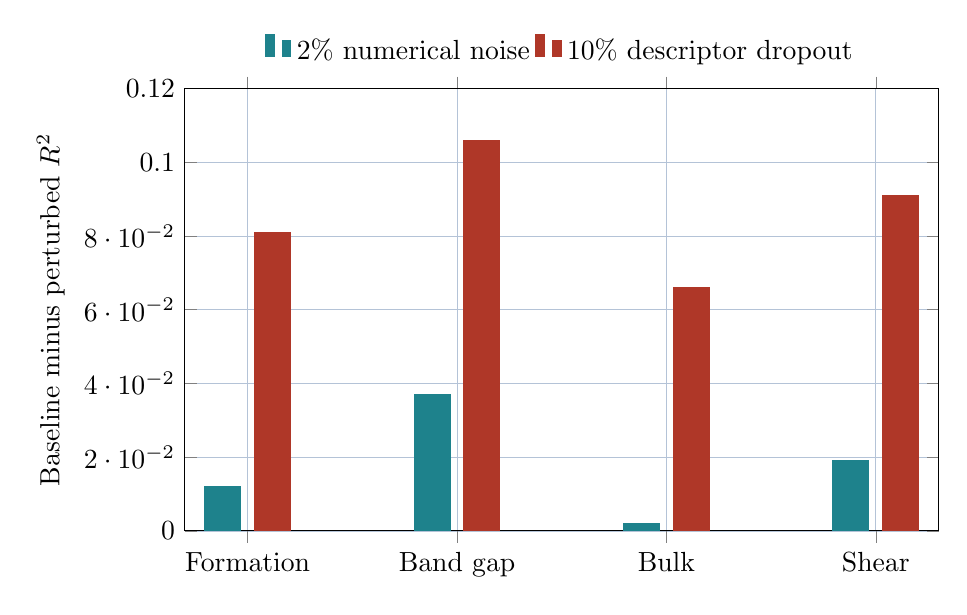
\begin{tikzpicture}
\begin{axis}[width=0.92\textwidth, height=7.2cm, ybar=5pt, bar width=13pt, ymin=0, ymax=0.12, ylabel={Baseline minus perturbed $R^2$}, symbolic x coords={ Formation, Band gap, Bulk, Shear }, xtick=data, legend style={ at={(0.5,1.03)}, anchor=south, legend columns=2, draw=none }, grid=major, grid style={ draw=geoMid, line width=0.25pt }]
\addplot[
    fill=geoTeal,
    draw=geoTeal
]
coordinates {
    (Formation,0.012)
    ({Band gap},0.037)
    (Bulk,0.002)
    (Shear,0.019)
};
\addplot[
    fill=geoRust,
    draw=geoRust
]
coordinates {
    (Formation,0.081)
    ({Band gap},0.106)
    (Bulk,0.066)
    (Shear,0.091)
};
\legend{
    2\% numerical noise,
    10\% descriptor dropout
}
\end{axis}
\end{tikzpicture}



\caption{JARVIS Extra Trees perturbation response under 2\% Gaussian noise and 10\% descriptor dropout. Input noise produces moderate performance degradation ($\Delta R^2 \le 0.037$), whereas descriptor dropout causes substantial accuracy loss ($\Delta R^2 \ge 0.066$) across all property targets.}



\label{fig:jarvis-perturbation}
\end{figure}

Target-specific descriptors increased baseline signal.



In some routes,

they also increased dropout dependence.



This shows that added predictive information is not automatically added

robustness.





\section{Initial descriptor-response patterns}



The leading common-lane responses differed by target.



The recorded patterns included:



\begin{itemize}



\item

formation energy:

site count,

volume per atom

and density;



\item

band gap:

site count,

density

and magnetisation;



\item

bulk and shear modulus:

volume per atom

and density among the strongest responses;



\item

target-specific band gap:

formation energy as a leading response.



\end{itemize}



These patterns are compatible with a conditional physical chain:



\begin{itemize}



\item

composition and energetic organisation influence electronic state;



\item

packing proxies carry information about volumetric and shear

response;



\item

different properties expose different accessible parts of the

representation.



\end{itemize}



Compatibility is not causality.



The result identifies candidate relationships for stronger tests.



It does not establish a universal hierarchy.





\begin{table}[H]



\centering



\caption{Bounded interpretation of initial JARVIS descriptor-response patterns.}



\label{tab:jarvis-descriptor-patterns}



\begin{tabularx}{\textwidth}{L{0.20\textwidth}
    L{0.28\textwidth}
    Y
}
\toprule
\textbf{Target}
&
\textbf{Observed leading responses}
&
\textbf{Bounded interpretation}
\\
\midrule
Formation energy
&
Site count,
volume per atom,
density.
&
Energetic prediction uses composition and packing-related routes;
necessity and causal direction remain unestablished.
\\
\addlinespace
Band gap
&
Site count,
density,
magnetisation;
formation energy in the target-specific lane.
&
Electronic prediction benefits from energetic and structural context;
the result is target- and model-conditioned.
\\
\addlinespace
Bulk modulus
&
Volume per atom and density.
&
Packing-related variables carry accessible information about
volumetric stiffness.
\\
\addlinespace
Shear modulus
&
Volume per atom and density,
with weaker total recovery.
&
Coarse packing proxies retain signal,
but directional mechanical behaviour remains less accessible.
\\
\bottomrule
\end{tabularx}



\end{table}





\section{Fresh execution and predecessor-linked replay}



The fresh execution completed:



\begin{equation}
48/48
\end{equation}



scientific units.



The predecessor-linked replay completed the same ordered plan under a

distinct execution identity.



The replay was interrupted during execution.



It resumed from verified controller-native checkpoints.



Only complete committed units were retained.





\section{Comparator defect and correction}



During replay adjudication,

a comparator defect was found.



A fallback identity key omitted descriptor-level dimensions.



Distinct descriptor-response rows could therefore be treated as

duplicates.



The scientific outputs were not rewritten.



The comparator was corrected through a named successor version.



The corrected comparator passed 50 tests and was applied read-only to

the immutable fresh and replay bundles.



This episode matters for two reasons.



First,

the initial comparison result could not be trusted until the identity

key was repaired.



Second,

the defect did not justify rerunning or silently replacing the

scientific execution.



The comparison instrument was corrected,

then applied again to the preserved evidence.





\begin{governingrule}



A defect in the adjudication layer must not be repaired by rewriting

the scientific evidence it was meant to inspect.



Correct the comparator.



Preserve the run.



Re-adjudicate read-only.



\end{governingrule}





\section{Replay result}



The final comparison included:



\begin{itemize}



\item

192 corresponding files;



\item

28,248 numerical cells.



\end{itemize}



The result was:



\begin{table}[H]



\centering



\caption{JARVIS fresh-versus-replay adjudication.}



\label{tab:jarvis-replay}



\begin{tabularx}{\textwidth}{L{0.28\textwidth}
    L{0.23\textwidth}
    Y
}
\toprule
\textbf{Contract}
&
\textbf{Result}
&
\textbf{Meaning}
\\
\midrule
Ordered plan identity
&
Pass
&
The same 48-unit scientific plan was completed.
\\
\addlinespace
Semantic identity
&
Pass
&
Corresponding values referred to the same scientific objects.
\\
\addlinespace
Numerical equivalence
&
Pass
&
All 28,248 compared numeric cells remained within
$10^{-10}$.
\\
\addlinespace
Maximum absolute difference
&
$1.07\times10^{-14}$
&
Maximum observed numerical divergence.
\\
\addlinespace
Raw-byte identity
&
Fail for 60 of 192 files
&
Scientific values reproduced,
but file bytes were not universally identical.
\\
\bottomrule
\end{tabularx}



\end{table}





The correct terminal description is:



\begin{quote}



Scientific replay equivalent,

byte divergent.



\end{quote}



The result does not establish cross-platform reproducibility.



It establishes local locked replay under the frozen environment and

tolerance.





\section{Runtime and resource accessibility}



The JARVIS fresh execution completed in approximately:



\begin{equation}
9.93
\ \mathrm{hours}.
\end{equation}



It used:



\begin{itemize}



\item

eight bounded workers;



\item

a consumer workstation;



\item

32 GB of installed RAM;



\item

no GPU dependency for the tabular execution.



\end{itemize}



The underlying JARVIS DFT calculations were not performed locally.



The runtime refers to the Geatomica modelling,

perturbation,

null,

removal

and evidence-generation workload over published records.











The machine remained available for ordinary use during much of the

run.



This is relevant to practical accessibility,

but it is not a formal benchmark.



The defensible conclusion is:



\begin{quote}



A bounded full-scale materials assurance workload completed locally on

ordinary workstation hardware without requiring dedicated accelerator

or cloud infrastructure.



\end{quote}





\section{What the JARVIS stage established}



The JARVIS stage supports the following bounded claims:



\begin{enumerate}



\item

All four targets contained meaningful non-null predictive signal under

the declared tabular routes.



\item

Target-specific admissible information improved performance.



\item

Larger populations improved prediction across all target/lane

aggregates.



\item

Model family materially changed the apparent explanatory structure.



\item

Population splitting changed performance,

and no universal hardest split was observed.



\item

Numerical noise and descriptor dropout exposed different forms of

sensitivity.



\item

The descriptor account was target-dependent.



\item

The complete scientific programme was reproduced by a predecessor-linked replay within

the frozen numerical tolerance.



\item

Numerical reproducibility did not imply raw-byte identity.



\item

An interrupted replay could resume from verified scientific-unit

boundaries.



\end{enumerate}





\section{What the JARVIS stage did not establish}



The stage did not establish:



\begin{itemize}



\item

physical causality;



\item

a universal descriptor hierarchy;



\item

material-by-material transfer;



\item

cross-source invariance;



\item

experimental validity;



\item

physical material-selection authority;



\item

universal zone thresholds;



\item

a completed reduced-complexity descriptor spine.



\end{itemize}





\begin{claimboundary}[JARVIS claim ceiling]



The JARVIS programme established a coherent,

non-null,

target-dependent and numerically replayable descriptor-response

surface within one governed calculated source environment.



It did not establish that the same response surface would survive a

second source.



That question required the Materials Project experiment.



\end{claimboundary}





\section{Chapter conclusion}



JARVIS demonstrated that Geatomica could operate at meaningful source

scale and return more than one predictive score.



The experiment separated:



\begin{itemize}



\item

target-dependent carrier signal;



\item

scale behaviour;



\item

population-transfer limits;



\item

model-conditioned explanation;



\item

noise and missingness sensitivity;



\item

scientific numerical replay;



\item

raw-byte divergence.



\end{itemize}



The result was promising,

but it remained source-local.



The next programme stage therefore changed the source environment.



That stage did not produce a simple clean validation.



It exposed the more difficult problem Geatomica had been built to

find.





% ============================================================

% END OF PART 2

%

% NEXT BLOCK:

%

% CHAPTER 5

% Materials Project and the Value of an Adverse Result

%

% CHAPTER 6

% Matbench, Magpie and Neural Transfer

%

% CHAPTER 7

% What Changed During the Programme

% ============================================================

% ============================================================

% PART 3

%

% CHAPTER 5

% Materials Project: When Predictive Signal Meets Unresolved Evidence

%

% CHAPTER 6

% Matbench, Magpie and Neural Transfer

%

% CHAPTER 7

% What Changed During the Programme

% ============================================================





% ============================================================

% CHAPTER 5

% ============================================================



\chapter{Materials Project: When Predictive Signal Meets Unresolved Evidence}

\begin{center}
\fbox{\begin{minipage}{0.91\textwidth}
\textbf{Question.} Can a route beat a paired broken-target comparator while still failing a minimal absolute predictive baseline?\\
\textbf{Comparison.} For the same 288 eligible elastic cells, paired-null separation was compared with held-out $R^2>0$.\\
\textbf{Result.} 211/288 (73.3\%) beat the paired null, but only 13/288 (4.51\%) achieved positive $R^2$ and passed both; median route $R^2$ was $-2.248$.\\
\textbf{Decision.} Require non-null signal and absolute viability separately; hold unresolved elastic source semantics.\\
\textbf{Boundary.} The $R^2>0$ boundary is the minimal demonstrated reference for this audit, not a universal engineering threshold.
\end{minipage}}
\end{center}




\label{chap:materials-project}





\section{Why move to a second source?}



The JARVIS programme established that Geatomica could execute a

complete four-target audit,

retain target-dependent behaviour

and reproduce the scientific response surface under a locked replay.



That result was necessary.



It was not sufficient.



A descriptor account that survives only inside one calculated database

may reflect:



\begin{itemize}



\item

the material population selected by that source;



\item

the source's calculation methods;



\item

its convergence and admission rules;



\item

its reporting conventions;



\item

its available descriptor fields;



\item

its historical database construction.



\end{itemize}



If descriptor authority was to mean more than source-local stability,

the audit had to enter a second computational environment.



The Materials Project therefore served two roles.



First,

it tested whether energetic and electronic descriptor behaviour would

recur across a separate source population.



Second,

it tested whether the assurance logic could survive a less cooperative

result.



The first role produced bounded support.



The second changed the programme.





\begin{governingrule}



A second source is not valuable only when it confirms the first.



It is equally valuable when it reveals that the original evidence

contract was incomplete.



\end{governingrule}





\section{The Materials Project programme}



The Materials Project stage retained the four-property structure:



\begin{itemize}



\item

formation energy;



\item

band gap;



\item

bulk modulus;



\item

shear modulus.



\end{itemize}



The programme expanded to:



\begin{equation}
64
\end{equation}



fresh scientific units and:



\begin{equation}
64
\end{equation}



replay units.



The source universe contained approximately:



\begin{equation}
154{,}377
\end{equation}



unique material records,

with target-specific cohorts constructed according to field

availability and the frozen modelling contract.



Together,

the JARVIS and Materials Project programmes touched approximately:



\begin{equation}
230{,}370
\end{equation}



calculated source records while retaining the two databases as

separate evidence environments.



The programme did not merge JARVIS and Materials Project into one

homogeneous table.



That separation matters.



A combined table would increase sample size while obscuring which

behaviour belonged to which source environment.





\begin{table}[H]



\centering



\caption{Role and outcome of the Materials Project programme.}



\label{tab:mp-programme-summary}



\begin{tabularx}{\textwidth}{L{0.29\textwidth}
    L{0.22\textwidth}
    Y
}
\toprule
\textbf{Object}
&
\textbf{Observed value}
&
\textbf{Interpretation}
\\
\midrule
Approximate source universe
&
154,377 unique records
&
Materials Project source population used by the governed build.
\\
\addlinespace
Fresh scientific units
&
64/64
&
Complete execution.
\\
\addlinespace
Replay scientific units
&
64/64
&
Complete replay under a separate execution identity.
\\
\addlinespace
Formation-energy route
&
Bounded support
&
Predictive and descriptor behaviour remained coherent under the
declared source and split conditions.
\\
\addlinespace
Band-gap route
&
Bounded support
&
Cross-source energetic/electronic recurrence was observed at aggregate
level.
\\
\addlinespace
Raw elastic source
&
Source hold
&
Extreme and unresolved values prevented physical interpretation.
\\
\addlinespace
Elastic numerical replay
&
Replay hold
&
Completed,
but exceeded the frozen absolute tolerance in 916 numeric cells.
\\
\bottomrule
\end{tabularx}



\end{table}





\section{Energetic and electronic recurrence}



Formation energy and band gap produced coherent bounded results.



At full scale,

median \Rtwo{} increased from:



\begin{equation}
0.675
\rightarrow
0.747
\end{equation}



for formation energy when target-specific admissible descriptors were

added.



For band gap,

the corresponding increase was:



\begin{equation}
0.559
\rightarrow
0.719.
\end{equation}



Signal persisted under composition and chemical-system holdouts,

although performance attenuated.



This broadly recurred with the JARVIS energetic and electronic pattern:



\begin{itemize}



\item

target-specific information increased recoverable signal;



\item

harder population splits reduced performance;



\item

the descriptor account remained conditional on source,

model

and population geometry;



\item

energetic and electronic targets remained more coherent than the raw

elastic routes.



\end{itemize}



The result supports cross-source recurrence at the population level.



It does not establish matched-material transfer.



Only nine exact structure fingerprints overlapped under the strict

matching route.



The two sources therefore act as provenance-separated witnesses,

not as two measurements of the same large set of materials.





\begin{claimboundary}[Cross-source recurrence boundary]



The Materials Project and JARVIS results support a bounded statement

that similar energetic and electronic modelling behaviour recurred

across two independently governed calculated source environments.



They do not establish that an individual material carries the same

descriptor response across both sources.



\end{claimboundary}





\section{Availability is not admissibility}



The elastic route exposed a more fundamental problem.



The source contained populated elastic fields.



That did not establish that every value was physically or numerically

fit for interpretation.



Before a model can answer what an elastic population means,

the source population must first establish:



\begin{itemize}



\item

material identity;



\item

property definition;



\item

units;



\item

calculation method;



\item

tensor or scalar status;



\item

sign meaning;



\item

Voigt,

Reuss

and Hill consistency;



\item

physical bounds;



\item

whether extreme values represent unstable structures,

failed calculations,

parsing defects

or sentinel values.



\end{itemize}



The original modelling route had treated field availability as

sufficient for intake.



The experiment showed that this assumption was too weak.



The source itself became the object of study.





\begin{engineeringconsequence}



An engineer cannot interpret a model's elastic ranking before deciding

whether the target population is physically and numerically admissible.



The model cannot repair the meaning of the source after fitting.



\end{engineeringconsequence}





\section{The elastic-source anomalies and semantic uncertainty}



The raw elastic routes exposed values at extreme scales.



Reported bulk-modulus values extended to approximately:



\begin{equation}
-4.70\times10^{11}
\ \mathrm{GPa},
\end{equation}



while reported shear values extended from approximately:



\begin{equation}
-1.43\times10^{13}
\ \mathrm{GPa}
\end{equation}



to:



\begin{equation}
5.65\times10^{13}
\ \mathrm{GPa}.
\end{equation}



Negative elastic quantities are not automatically database errors.



A mechanically unstable theoretical structure can produce negative

elastic behaviour.



A simple sign filter would therefore destroy potentially meaningful

physics.



The issue was the combination of:



\begin{itemize}



\item

extreme magnitude;



\item

uncertain source semantics;



\item

mixed sign behaviour;



\item

bound-order inconsistencies;



\item

large influence on prediction and replay.



\end{itemize}



These values dominated:



\begin{itemize}



\item

loss functions;



\item

tree partitions;



\item

model comparisons;



\item

feature rankings;



\item

numerical replay sensitivity.



\end{itemize}



A model trained on this population could still learn structure.



That did not mean the resulting structure was physically

interpretable.





\begin{figure}[H]



\centering



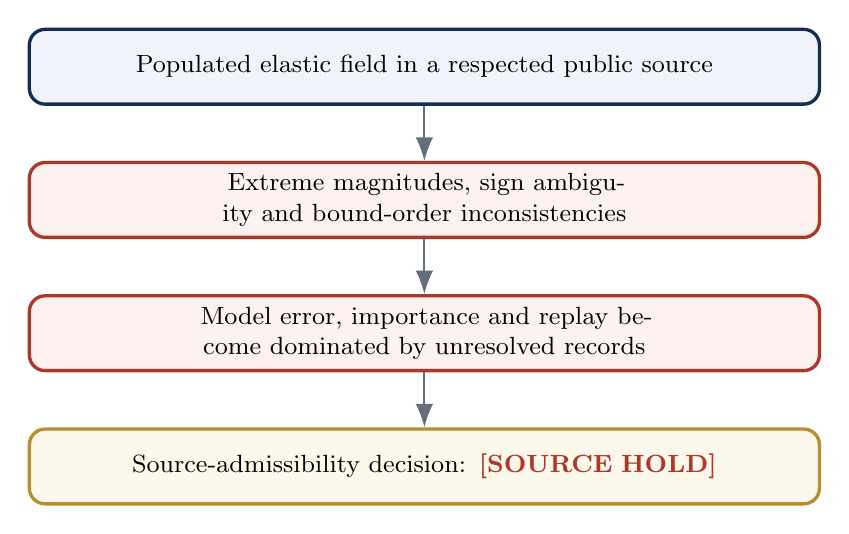
\begin{tikzpicture}[node distance=7mm, every node/.style={ font=\small, align=center }, stage/.style={ draw=geoBlue, very thick, rounded corners=2mm, fill=geoLight, text width=9.8cm, minimum height=0.95cm }, warning/.style={ draw=geoRust, very thick, rounded corners=2mm, fill=geoRedLight, text width=9.8cm, minimum height=0.95cm }, outcome/.style={ draw=geoGold, very thick, rounded corners=2mm, fill=geoGoldLight, text width=9.8cm, minimum height=0.95cm }]
\node[stage] (field) {
    Populated elastic field in a respected public source
};
\node[
    warning,
    below=of field
] (extreme) {
    Extreme magnitudes,
    sign ambiguity
    and bound-order inconsistencies
};
\node[
    warning,
    below=of extreme
] (model) {
    Model error,
    importance
    and replay become dominated by unresolved records
};
\node[
    outcome,
    below=of model
] (hold) {
    Source-admissibility decision:
    \sourcehold{}
};
\draw[
    -{Latex[length=3mm]},
    thick,
    color=geoGrey
]
(field) -- (extreme);
\draw[
    -{Latex[length=3mm]},
    thick,
    color=geoGrey
]
(extreme) -- (model);
\draw[
    -{Latex[length=3mm]},
    thick,
    color=geoGrey
]
(model) -- (hold);
\end{tikzpicture}



\caption{The elastic failure occurred before interpretation. A populated source field entered the modelling route, but unresolved physical and numerical semantics prevented the resulting model evidence from acquiring authority.}



\label{fig:mp-admission-failure}



\end{figure}






\begin{figure}[H]
\centering
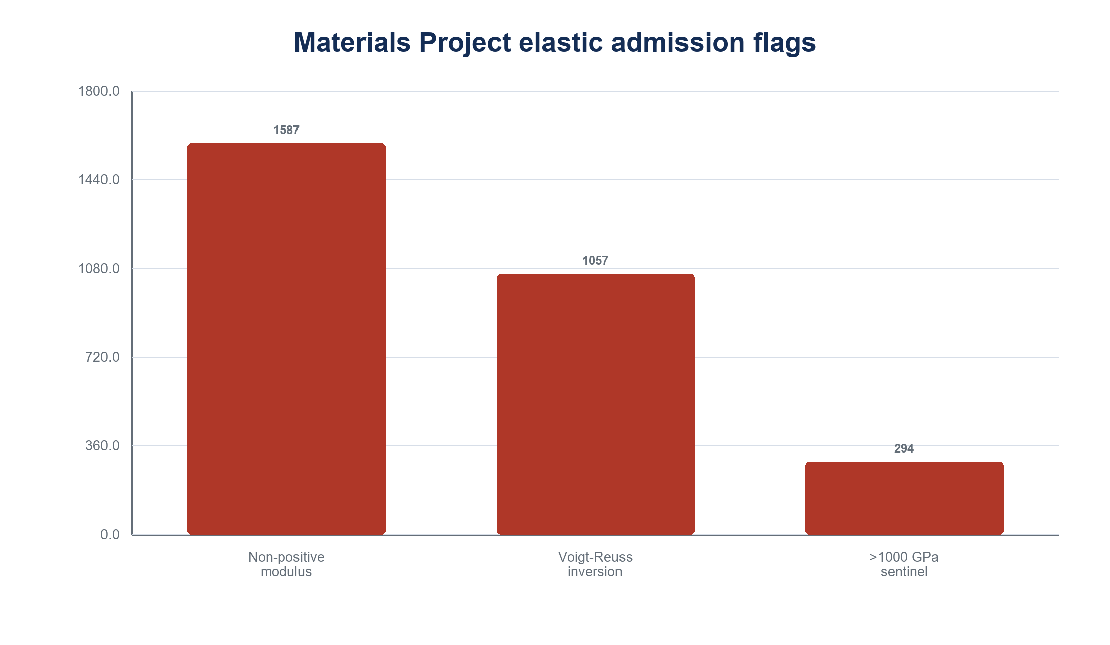
\includegraphics[width=0.92\textwidth]{figures/mp_elastic_admission_flags.pdf}
\caption{\textbf{HISTORICAL REPORT BOUND; SOURCE HOLD.} Elastic admission flags reported for the Materials Project route. Classes can overlap and begin adjudication; they do not prove that every flagged record is corrupt.}
\label{fig:mp-elastic-admission-evidence-edition}
\end{figure}

\section{The prospective no-fit admission audit}



A successor no-fit admission classifier evaluated:



\begin{equation}
26{,}056
\end{equation}



elastic record-target pairs.



The audit classified:



\begin{equation}
2{,}165
\end{equation}



pairs as anomalous and unresolved under the declared rules.



Observed anomaly classes included:



\begin{itemize}



\item

1,587 non-positive scalar cases;



\item

1,057 Voigt/Reuss order reversals;



\item

294 values above a

\SI{1000}{\giga\pascal}

review sentinel.



\end{itemize}



These classes overlap.



Their counts should not be added as mutually exclusive categories.



The audit also identified an example associated with

\(\mathrm{TiCo}_{2}\)

at an extreme reported magnitude of approximately:



\begin{equation}
-9.40\times10^{11}
\ \mathrm{GPa}.
\end{equation}



The no-fit classifier did not claim that every flagged record was

scientifically invalid.



It separated records that could not proceed directly into ordinary

interpretation without source resolution.





\begin{table}[H]



\centering



\caption{Prospective admission classification for the Materials Project elastic record-target pairs.}



\label{tab:mp-admission}



\begin{tabularx}{\textwidth}{L{0.29\textwidth}
    C{0.17\textwidth}
    Y
}
\toprule
\textbf{Admission class}
&
\textbf{Count}
&
\textbf{Meaning}
\\
\midrule
\texttt{ADMISSIBLE\_CONDITIONAL}
&
23,891
&
Scalar property present,
but complete tensor and record-level method context were not sufficient
for unconditional physical interpretation.
\\
\addlinespace
\texttt{ANOMALOUS\_UNRESOLVED}
&
2,165
&
At least one declared sign,
bound-order
or extreme-value rule required resolution before modelling authority.
\\
\addlinespace
\texttt{ADMISSIBLE\_STABLE}
&
0
&
No record met the stronger stable-admission condition under the
available source evidence.
\\
\bottomrule
\end{tabularx}



\end{table}





The most important change was procedural.



The audit moved admission before fitting.



A later model could no longer legitimise an earlier unresolved source

population merely by producing a useful score.





\begin{governingrule}



Availability answers whether a field exists.



Admission answers whether that field is fit for the scientific claim

being requested.



These are separate gates.



\end{governingrule}





\section{The database was not the failure}



The result should not be interpreted as a claim that the Materials

Project is a failed database.



Large public scientific databases necessarily contain:



\begin{itemize}



\item

edge cases;



\item

unstable calculated structures;



\item

heterogeneous historical records;



\item

evolving calculation methods;



\item

partial fields;



\item

legacy conventions;



\item

values whose meaning depends on source-specific context.



\end{itemize}



These conditions are part of real scientific infrastructure.



The failure would be to treat a large public database as if every

populated field formed one immediately homogeneous and physically

interpretable population.



The source provided evidence.



The modelling route had to decide what kind of evidence it was.





\section{The elasticity paradox}



The elastic route exposed another failure that was independent of

source admission.



Across the raw untransformed elasticity programme:



\begin{equation}
88.0\%
\end{equation}



of model cells achieved positive valid-minus-null separation:

This 88.0\% figure describes the earlier historical raw-elasticity audit under its own eligibility boundary. It is not the same-denominator analysis in Paper~2, where 211 of 288 cells (73.3\%) had positive paired-null separation and 13 of 288 (4.51\%) had positive held-out $R^2$.



\begin{equation}
S>0.
\end{equation}



On that basis,

the original aggregation rule treated much of the route as supported.



However,

median baseline predictive performance remained negative:



\begin{equation}
R^2<0.
\end{equation}



The valid model had learned more than the paired target-permutation

null.



It had not learned enough to outperform prediction of the dataset

mean.



The same model result therefore supported two statements:



\begin{enumerate}



\item

non-random signal exists under the declared comparison;



\item

the resulting model is still absolutely unusable.



\end{enumerate}



The first statement did not cancel the second.





\begin{figure}[H]



\centering



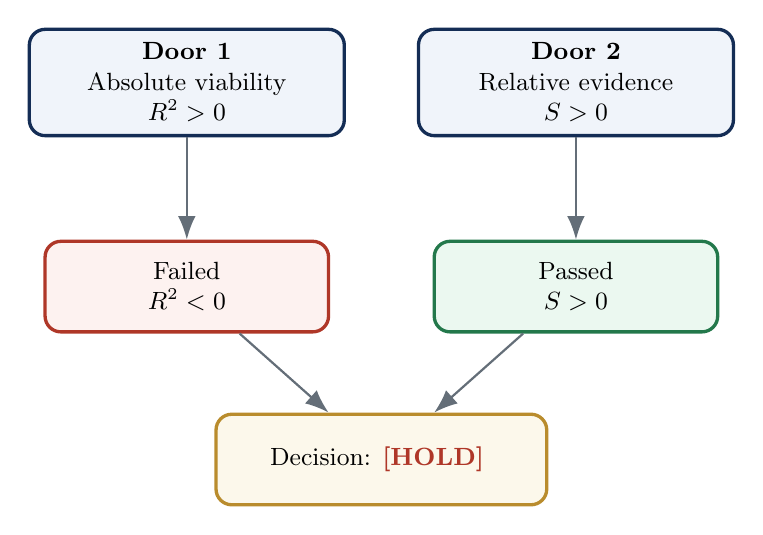
\begin{tikzpicture}[node distance=10mm and 9mm, every node/.style={ font=\small, align=center }, door/.style={ draw=geoBlue, very thick, rounded corners=2mm, fill=geoLight, minimum width=4.0cm, minimum height=1.35cm }, pass/.style={ draw=geoGreen, very thick, rounded corners=2mm, fill=geoGreenLight, minimum width=3.6cm, minimum height=1.15cm }, fail/.style={ draw=geoRust, very thick, rounded corners=2mm, fill=geoRedLight, minimum width=3.6cm, minimum height=1.15cm }, decision/.style={ draw=geoGold, very thick, rounded corners=2mm, fill=geoGoldLight, minimum width=4.2cm, minimum height=1.15cm }]
\node[door] (d1) {
    \textbf{Door 1}\\
    Absolute viability\\
    $R^2>0$
};
\node[
    door,
    right=of d1
] (d2) {
    \textbf{Door 2}\\
    Relative evidence\\
    $S>0$
};
\node[
    fail,
    below=13mm of d1
] (f1) {
    Failed\\
    $R^2<0$
};
\node[
    pass,
    below=13mm of d2
] (p2) {
    Passed\\
    $S>0$
};
\node[
    decision,
    below=16mm of $(f1)!0.5!(p2)$
] (hold) {
    Decision:
    \hold{}
};
\draw[
    -{Latex[length=3mm]},
    thick,
    color=geoGrey
]
(d1) -- (f1);
\draw[
    -{Latex[length=3mm]},
    thick,
    color=geoGrey
]
(d2) -- (p2);
\draw[
    -{Latex[length=3mm]},
    thick,
    color=geoGrey
]
(f1) -- (hold);
\draw[
    -{Latex[length=3mm]},
    thick,
    color=geoGrey
]
(p2) -- (hold);
\end{tikzpicture}



\caption{The two-door model-viability gate. Positive null separation cannot repair failed absolute prediction. Both doors must pass before bounded interpretation is nominated.}



\label{fig:two-door-mp}



\end{figure}





\section{Why the paradox matters physically}



A relative-only pass can still change an engineering decision if it is

reported carelessly.



Imagine a model used to prioritise candidate materials for:



\begin{itemize}



\item

additional DFT calculation;



\item

synthesis;



\item

mechanical testing;



\item

high-temperature exposure;



\item

microscopy;



\item

neutron or synchrotron characterisation;



\item

prototype fabrication.



\end{itemize}



If the model beats a deliberately weakened null,

the result may be described as evidence that the screening route works.



If the model remains worse than predicting the mean,

that description is not enough.



The engineer may still spend:



\begin{itemize}



\item

compute time;



\item

laboratory time;



\item

material stock;



\item

machine access;



\item

staff effort;



\item

experimental budget;



\item

calendar time.



\end{itemize}



The two-door rule therefore changes what is allowed to happen next.



It is not merely a change in terminology.





\begin{engineeringconsequence}



A model that passes only the relative-evidence door may justify further

diagnosis.



It does not justify engineering use.



\end{engineeringconsequence}





\section{The successor viability rule}



The corrected rule requires:



\begin{equation}
\text{viable}
\iff
\left(
R^2>0
\right)
\land
\left(
S>0
\right).
\end{equation}



The original aggregation was preserved as historical evidence.



The corrected rule was introduced under a successor protocol.



The result was not rewritten to imply that the gate had always existed.



This matters because the programme itself is part of the evidence.



A scientific method that changes after observing a failure must retain

the sequence:



\begin{enumerate}



\item

original rule;



\item

observed defect;



\item

preserved historical output;



\item

successor rule;



\item

new claim boundary.



\end{enumerate}





\section{Fresh execution and replay}



The Materials Project fresh execution completed:



\begin{equation}
64/64
\end{equation}



scientific units.



The replay also completed:



\begin{equation}
64/64
\end{equation}



units.



The numerical comparison covered:



\begin{equation}
37{,}924
\end{equation}



cells.



Of these:



\begin{equation}
916
\end{equation}



exceeded the frozen absolute tolerance of:



\begin{equation}
10^{-10}.
\end{equation}



Every exceedance occurred in bulk- or shear-modulus routes.



Formation energy and band gap remained within the tolerance.





\begin{table}[H]



\centering



\caption{Materials Project replay outcome by evidence route.}



\label{tab:mp-replay-outcome}



\begin{tabularx}{\textwidth}{L{0.23\textwidth}
    L{0.23\textwidth}
    Y
}
\toprule
\textbf{Route}
&
\textbf{Replay state}
&
\textbf{Interpretation}
\\
\midrule
Formation energy
&
Numerical pass
&
Fresh and replay values remained within the frozen tolerance.
\\
\addlinespace
Band gap
&
Numerical pass
&
Fresh and replay values remained within the frozen tolerance.
\\
\addlinespace
Bulk modulus
&
Replay hold
&
At least part of the compared response exceeded the frozen absolute
tolerance.
\\
\addlinespace
Shear modulus
&
Replay hold
&
At least part of the compared response exceeded the frozen absolute
tolerance.
\\
\bottomrule
\end{tabularx}



\end{table}





The elastic replay still preserved:



\begin{itemize}



\item

model-family ordering;



\item

leading descriptor ordering;



\item

null-separation signs;



\item

baseline-sign conclusions.



\end{itemize}



The scientific pattern recurred.



The strict numerical contract failed.



Both results were retained.





\begin{governingrule}



A stable scientific ordering does not repair a failed numerical replay

contract.



A failed numerical replay contract does not erase every repeated

scientific pattern.



Mixed evidence must remain mixed.



\end{governingrule}





\section{Why the tolerance was not widened}



After observing the replay divergence,

it would have been possible to argue that an absolute tolerance of:



\begin{equation}
10^{-10}
\end{equation}



was unnecessarily strict for targets spanning extreme magnitudes.



That may be true.



It does not justify changing the predeclared contract after seeing

the result.



The correct procedure is:



\begin{enumerate}



\item

retain the original failed adjudication;



\item

diagnose whether absolute,

relative

or scale-normalised tolerance is more appropriate;



\item

define a successor replay contract;



\item

execute the successor under a new identity;



\item

compare the conclusions without rewriting the original result.



\end{enumerate}



The Materials Project elastic replay therefore remains held under the

original contract.





\section{What changed during the Materials Project stage}



The Materials Project experiment changed the programme in five ways.



\subsection{Admission moved before fitting}



A populated source field could no longer enter ordinary interpretation

without a declared admissibility decision.



\subsection{Relative evidence was separated from absolute viability}



Positive null separation could no longer authorise an unusable model.



\subsection{Mixed states replaced one terminal success label}



Formation energy,

band gap,

bulk modulus

and shear modulus could return different evidence states inside the

same completed programme.



\subsection{Reproducibility became multi-contract}



Semantic recurrence,

numerical equivalence

and byte identity were treated separately.



\subsection{A negative result became an engineering output}



The hold was not a failed attempt to find a positive story.



It was the correct terminal result for the available evidence.





\begin{evidencebox}[Materials Project terminal evidence state]



\begin{itemize}



\item

Formation energy:

bounded cross-source support and numerical replay pass.



\item

Band gap:

bounded cross-source support and numerical replay pass.



\item

Raw elasticity:

source-admissibility hold.



\item

Elastic strict replay:

hold under the frozen absolute tolerance.



\item

Historical outputs:

preserved.



\item

Successor protocol:

required for any revised elastic admission or replay rule.



\end{itemize}



\end{evidencebox}





\section{What the Materials Project stage established}



The Materials Project stage supports the following bounded claims:



\begin{enumerate}



\item

Energetic and electronic modelling behaviour recurred at aggregate

level across JARVIS and Materials Project.



\item

Cross-source recurrence did not eliminate split,

model

or representation dependence.



\item

A populated elastic field was not automatically admissible for

physical interpretation.



\item

The prospective admission layer identified a substantial unresolved

record class.



\item

Positive separation from a paired null was insufficient for model

viability.



\item

The two-door rule was required to separate non-random signal from

usable prediction.



\item

Fresh and replay executions can preserve scientific ordering while

failing a stricter numerical contract.



\item

A completed scientific programme can return a valid hold.



\end{enumerate}





\section{What the Materials Project stage did not establish}



The stage did not establish:



\begin{itemize}



\item

that every flagged elastic record is erroneous;



\item

that negative modulus values are intrinsically invalid;



\item

that the Materials Project is an unreliable scientific source;



\item

that elasticity is inherently unpredictable;



\item

that cross-source recurrence implies matched-material agreement;



\item

that log transformation is universally correct;



\item

that the successor admission rules have been externally validated;



\item

that a held route can never be recovered through better source

resolution.



\end{itemize}





\begin{claimboundary}[Materials Project claim ceiling]



The Materials Project stage reduced confidence in single-number

evidence.



It did not reduce confidence in scientific modelling itself.



The result showed that predictive signal,

source meaning,

absolute viability

and replay equivalence must be adjudicated separately.



\end{claimboundary}





\section{Chapter conclusion}



The Materials Project stage did not provide a simpler repetition of

JARVIS.



It exposed the boundaries that the first complete audit could not

reveal by itself.



The strongest result was not a new regressor.



It was a change in what counted as evidence.



A source field had to be admitted.



A model had to be absolutely useful.



A null had to fail in the expected direction.



A replay had to satisfy its own declared contract.



A mixed scientific programme had to be allowed to return a smaller

honest answer.



The next stage entered a deliberately curated benchmark environment.



The question was no longer whether raw scientific evidence could fail.



It was whether strong benchmark performance would make the assurance

problem disappear.







% ============================================================

% CHAPTER 6

% ============================================================




\chapter[Matbench Neural Assurance]{Matbench:\ Sealed Fresh Assurance and Exact Repeat}

\begin{center}
\fbox{\begin{minipage}{0.91\textwidth}
\textbf{Question.} Does fitted permutation importance agree with complete retrained-removal consequence?\\
\textbf{Comparison.} Across four official Matbench tasks, 142 Magpie descriptors and five folds, fitted importance was compared with refitted individual and group removals under one frozen CPU-MLP protocol.\\
\textbf{Result.} Mean Spearman agreement was 0.039404 and mean top-10 overlap was 0.100; all 3,440 fresh and 3,440 repeat units matched exactly across 65,740 numeric cells.\\
\textbf{Decision.} Treat fitted use and retrained dependence as different measurements.\\
\textbf{Boundary.} The result is same-environment repeatability under one representation/model protocol, not causal necessity or external replication.
\end{minipage}}
\end{center}


\section{Evidence transition}

The previous edition described Matbench V0.3 only as an active operational
patch. The fresh execution has now reached \textbf{MEASURED LOCAL} terminal
state: all 3,440 predeclared units completed and the final manifest sealed.
The separately identified repeat completed all 3,440 units under a distinct
execution identity. All 65,740 compared numeric cells were exactly equal and
semantic identity passed for every unit. This chapter therefore treats
same-environment repeatability as measured while withholding external replication.

The execution used four official Matbench regression tasks, five official folds,
142 composition-derived Magpie features, and a fixed scikit-learn
\texttt{MLPRegressor(128,64)} route. It contained 20 baseline/perturbation
units, 2,840 retrained individual-feature removals and 580 retrained
property-group removals. accepted evidence memory was disabled and recorded zero promotions.

\section{Predictive carrier}

\begin{figure}[H]
\centering
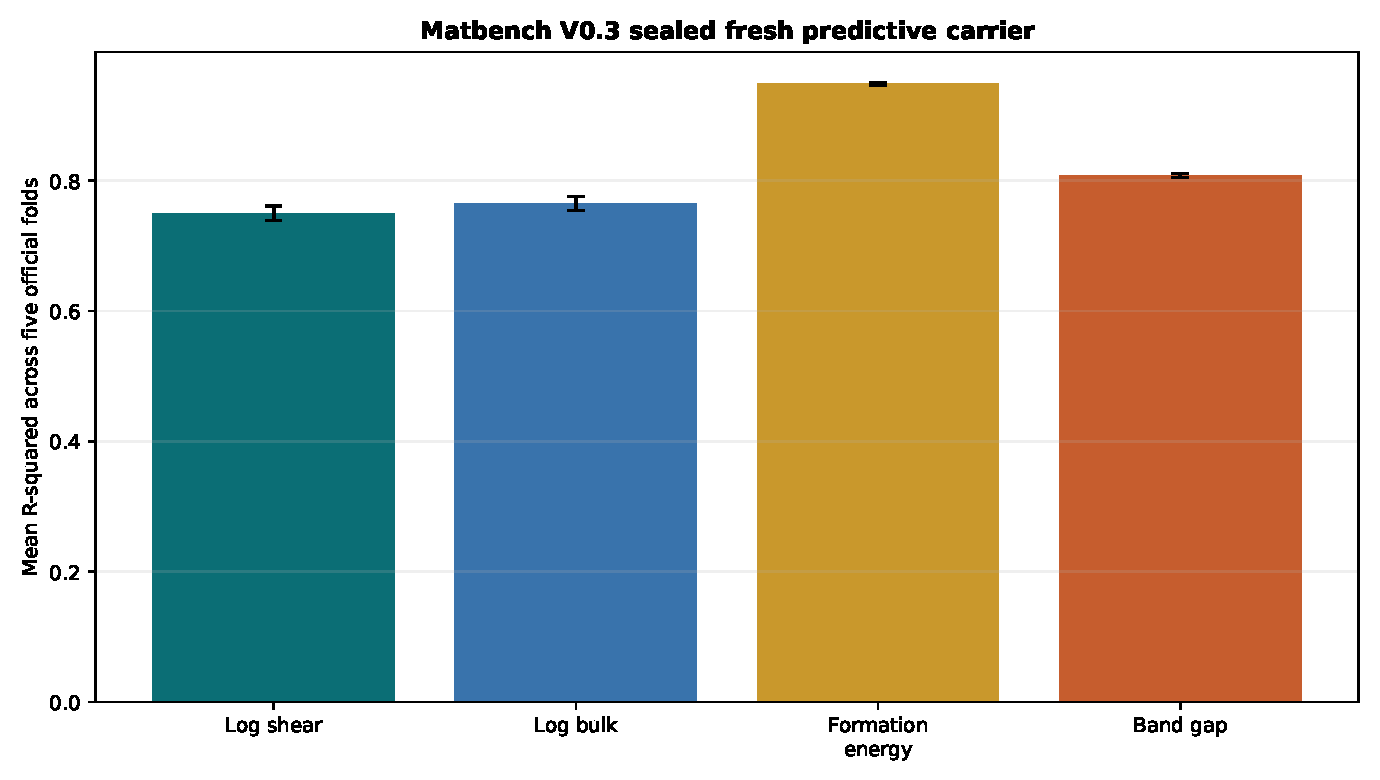
\includegraphics[width=0.90\textwidth]{figures/matbench_v03_fresh_baseline_r2.pdf}
\caption{\textbf{MEASURED LOCAL FRESH RUN.} Mean baseline predictive carrier
across five official folds. Error bars show fold standard deviation. Replay is
completed and established exact same-environment repeatability.}
\end{figure}

\begin{table}[H]
\centering
\small
\caption{Matbench V0.3 sealed fresh baseline results. MAE remains task-native and
must not be compared as one physical scale across targets.}
\begin{tabular}{lrrr}
\toprule
Task & Mean $R^2$ & SD $R^2$ & Mean MAE \\
\midrule
Formation energy & 0.9484 & 0.0017 & 0.1447 \\
Band gap & 0.8083 & 0.0033 & 0.4245 \\
Log bulk modulus & 0.7649 & 0.0104 & 0.1202 \\
Log shear modulus & 0.7504 & 0.0108 & 0.1334 \\
\bottomrule
\end{tabular}
\end{table}

The fixed neural carrier remained strongest for formation energy, followed by
band gap, logarithmic bulk modulus and logarithmic shear modulus. Two-percent
test-feature noise caused comparatively small mean MAE changes, while ten-percent
cell dropout caused much larger degradation in every task. The carrier therefore
survives small continuous disturbance better than broad missingness under this
declared route.

\section{Importance is not retrained-removal consequence}

\begin{figure}[H]
\centering
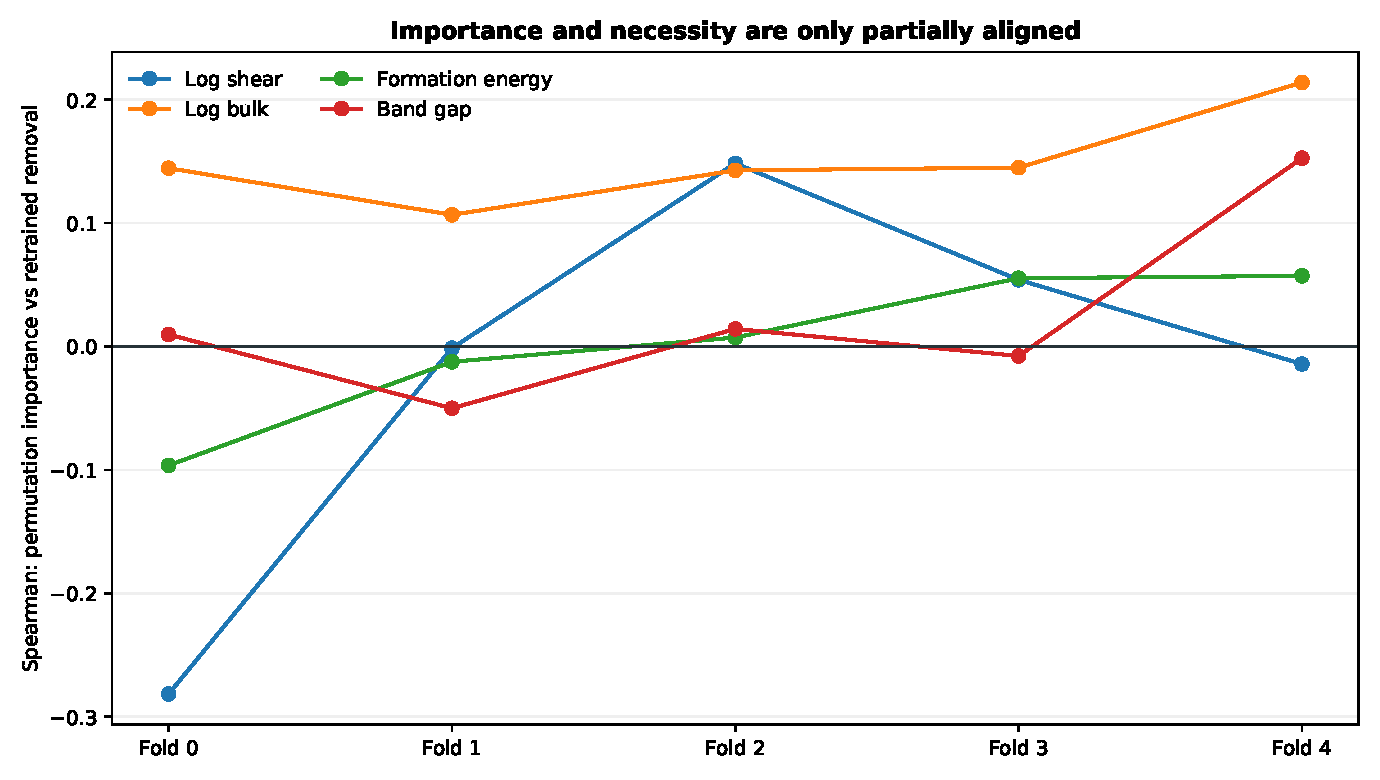
\includegraphics[width=0.90\textwidth]{figures/matbench_v03_importance_removal_spearman.pdf}
\caption{\textbf{MEASURED LOCAL FRESH RUN.} Fold-level Spearman association
between fitted permutation importance and independently retrained single-feature
removal consequence. Near-zero values indicate ranking disagreement, not causal
irrelevance.}
\end{figure}

Across the 20 task-fold views, the mean Spearman association between fitted
permutation MAE increase and retrained-removal MAE increase was
0.039, ranging from
-0.282 to 0.214.
The mean top-10 overlap was 10.0\%%.

\begin{figure}[H]
\centering
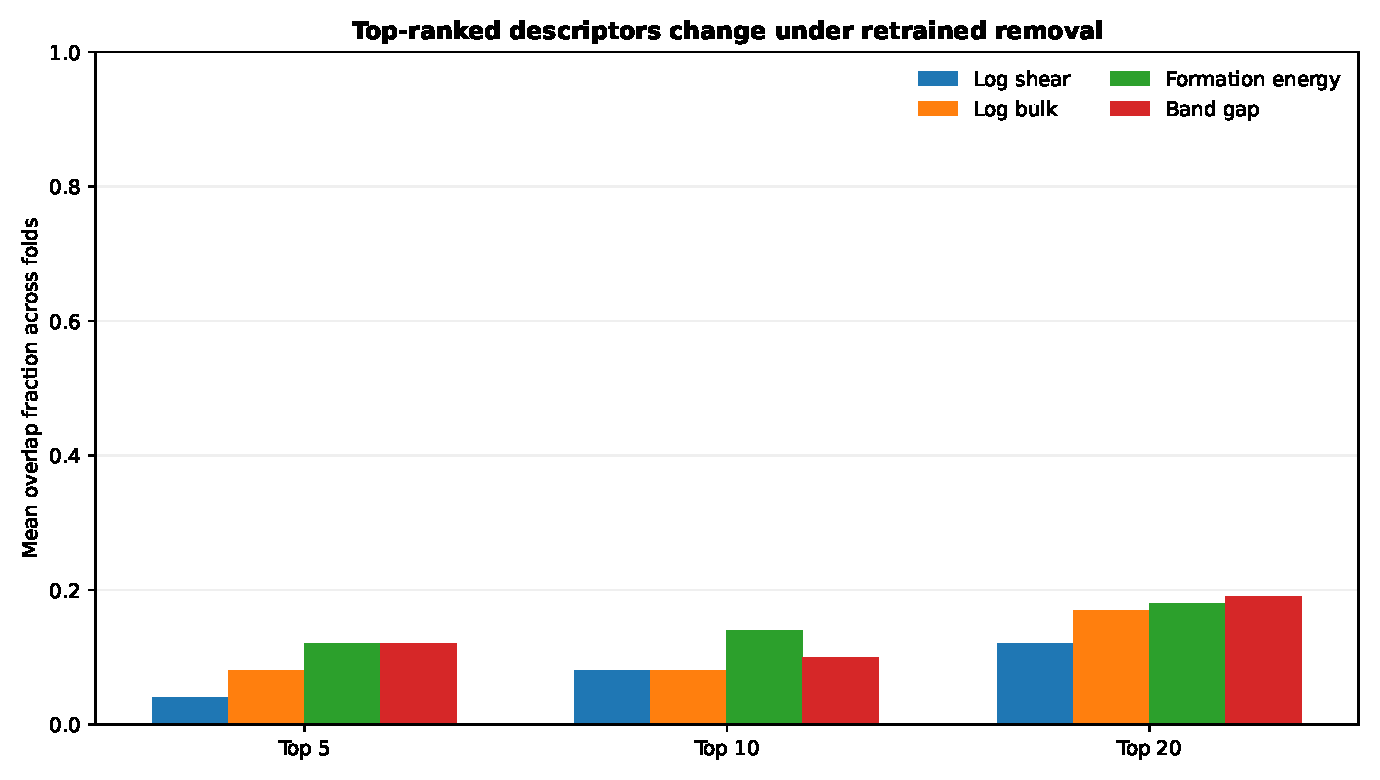
\includegraphics[width=0.90\textwidth]{figures/matbench_v03_topk_overlap.pdf}
\caption{\textbf{MEASURED LOCAL FRESH RUN.} Mean overlap between descriptors
ranked by fitted permutation response and descriptors ranked by retrained-removal
consequence at $k=5,10,20$.}
\end{figure}

The disagreement is not a subtle edge case. Of 2,840 individual removals,
1,781 improved MAE relative to the
matched baseline and 1,059 worsened it.
Of 580 group removals, 369 improved MAE
and 211 worsened it. A feature can therefore
be influential when disturbed in a fitted network without being necessary after
the model is retrained and allowed to redistribute signal.

\section{The necessary limitation}

The removal route changes the input dimensionality and refits the MLP. Although
the seed, fold and model contract are frozen, the current protocol contains no
sham full-feature refit ensemble that directly measures optimisation variance
without removing information. The observed disagreement can contain at least
three components: descriptor substitutability, changed optimisation trajectory,
and finite-sample variation. It is therefore evidence against treating fitted
importance as necessity, but it is not a clean quantitative estimate of how much
signal each descriptor uniquely contributes.

The next neural protocol should add repeated sham refits and matched random-column
controls before promoting any descriptor-level authority classification.

\section{Runtime and replay state}

The fresh execution ran for approximately 19.16 hours on the local CPU
workstation with two workers. Summed unit wall time was 37.94 hours, consistent
with approximately two-way bounded concurrency. The repeat required 20.60 hours,
used a new execution identity and did not reuse fresh outputs. The frozen
comparator passed, so the scientific state is:

\begin{center}
\textcolor{geoGreen}{\textbf{[PASS]}} \texttt{MEASURED LOCAL; REPLAYED SAME-ENVIRONMENT}
\end{center}

\section{Claim boundary}

Supported: a sealed 3,440-unit fresh execution showing strong predictive carrier
signal and substantial disagreement between fitted perturbation rankings and
retrained removal consequences under the declared Matbench tasks.

Not supported: external replication, unique descriptor
dependence, causal feature claims, engineering qualification, external validation,
or accepted evidence-memory promotion.


\chapter[Spatial GIL Persistence]{Spatial GIL:\ Representation Persistence at 256 Materials}

\begin{center}
\fbox{\begin{minipage}{0.91\textwidth}
\textbf{Question.} Did an initially promising angle-aware representation persist when the cohort increased to 256 materials?\\
\textbf{Comparison.} Simple and repaired angle-aware structural representations were compared across deterministic folds and bulk/shear targets.\\
\textbf{Result.} The earlier angle advantage did not persist reliably at 256 materials.\\
\textbf{Decision.} Reject automatic scale-up or GNN escalation; diagnose representation blocks first.\\
\textbf{Boundary.} This is a bounded local persistence test, not proof that angular structure is universally unimportant.
\end{minipage}}
\end{center}


\section{The next representation question}

The tabular programme asks whether an explanation survives disturbance in
descriptor space. Spatial GIL moves the intervention toward crystal structure.
The bounded V0.3 predecessor used 64 real JARVIS structures and found an apparent
advantage for a repaired complete-shell angle-aware representation over a simple
crystal-graph summary. The 256-material successor asked one narrower question:

\begin{quote}
Does that angle-aware advantage persist across four times the sample size and
four deterministic folds, and is any persistent gain larger for shear than bulk?
\end{quote}

No GNN, new target, feature search or automatic 512-material escalation was
authorised.

\section{Protocol and execution}

The result-blind cohort contains the first 256 ascending JARVIS identifiers with
finite bulk and shear labels and a well-formed structure. Four contiguous
64-material test folds were frozen over that order. Each fold used 192 training
records, Ridge with $alpha=10^-6$, and two representations:

\begin{itemize}
\item a nine-coordinate simple crystal-graph summary;
\item the same summary plus six density-normalised complete-shell angle bins.
\end{itemize}

Translation, rotation, atom permutation and supercell controls tested
representation preservation; a small coordinate jitter remained a declared
nonphysical positional-sensitivity stress. All 16 fresh units and all 16 replay
units sealed. Replay passed raw-byte, semantic-metadata and frozen-numerical
identity. The maximum representation-preserving prediction delta was
$6.82\times10^{-13}$, below the $10^{-10}$ gate. accepted evidence-memory promotions remained zero.

\section{The persistence result}

\begin{figure}[H]
\centering
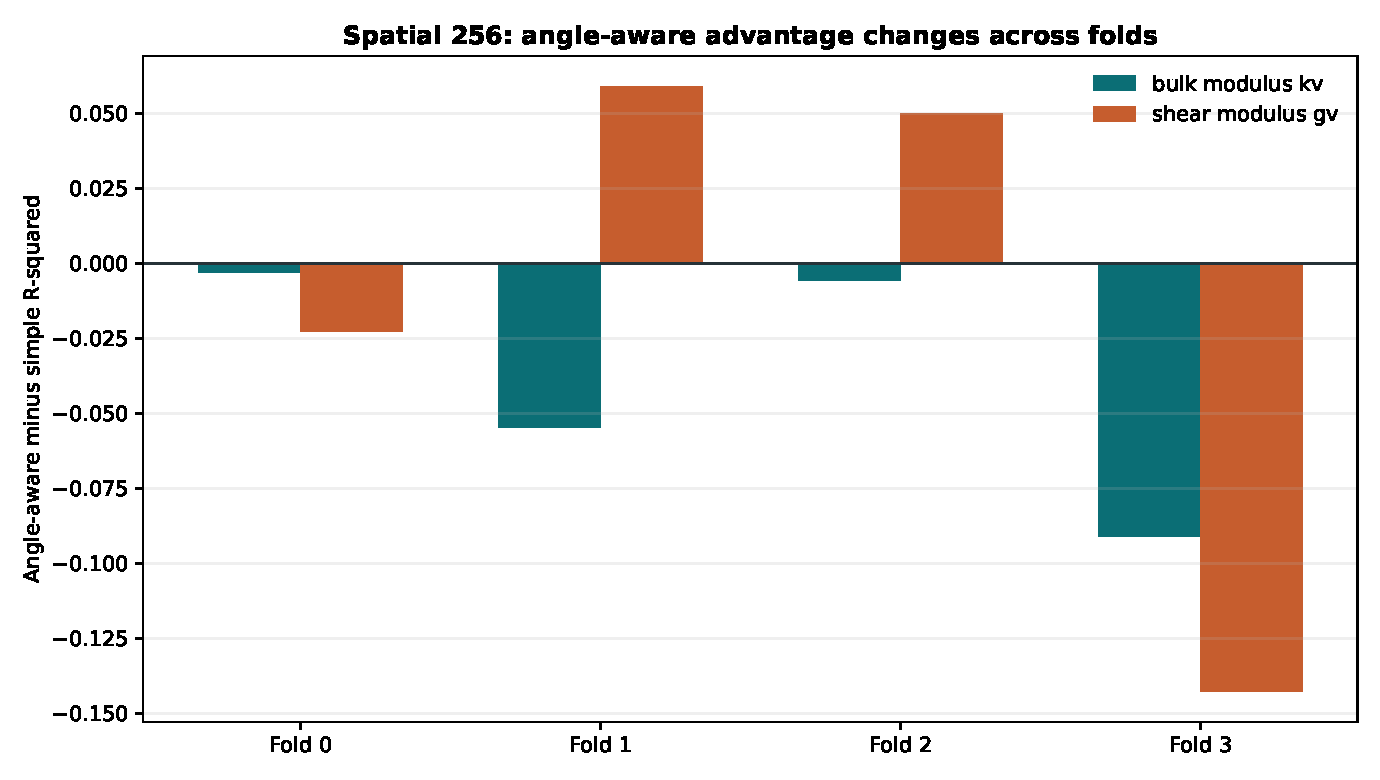
\includegraphics[width=0.90\textwidth]{figures/spatial_256_fold_delta_r2.pdf}
\caption{\textbf{SEALED AND REPLAYED LOCAL EVIDENCE.} Fold-level change in
$R^2$ when the six complete-shell angle bins are added to the simple graph
summary. Positive values favour the angle-aware representation.}
\end{figure}

The earlier 64-material direction did not persist. Bulk was worse with angle
features in all four folds. Shear improved in two folds and worsened in two,
including one large negative reversal.

\begin{table}[H]
\centering
\small
\caption{Pooled out-of-fold Spatial 256 performance.}
\begin{tabular}{lrrrr}
\toprule
Target & Simple $R^2$ & Angle $R^2$ & $\Delta R^2$ & MAE simple / angle \\
\midrule
Bulk modulus & 0.4447 & 0.4031 & -0.0416 & 35.00 / 36.40 \\
Shear modulus & 0.3758 & 0.3513 & -0.0244 & 20.69 / 21.26 \\
\bottomrule
\end{tabular}
\end{table}

\begin{figure}[H]
\centering
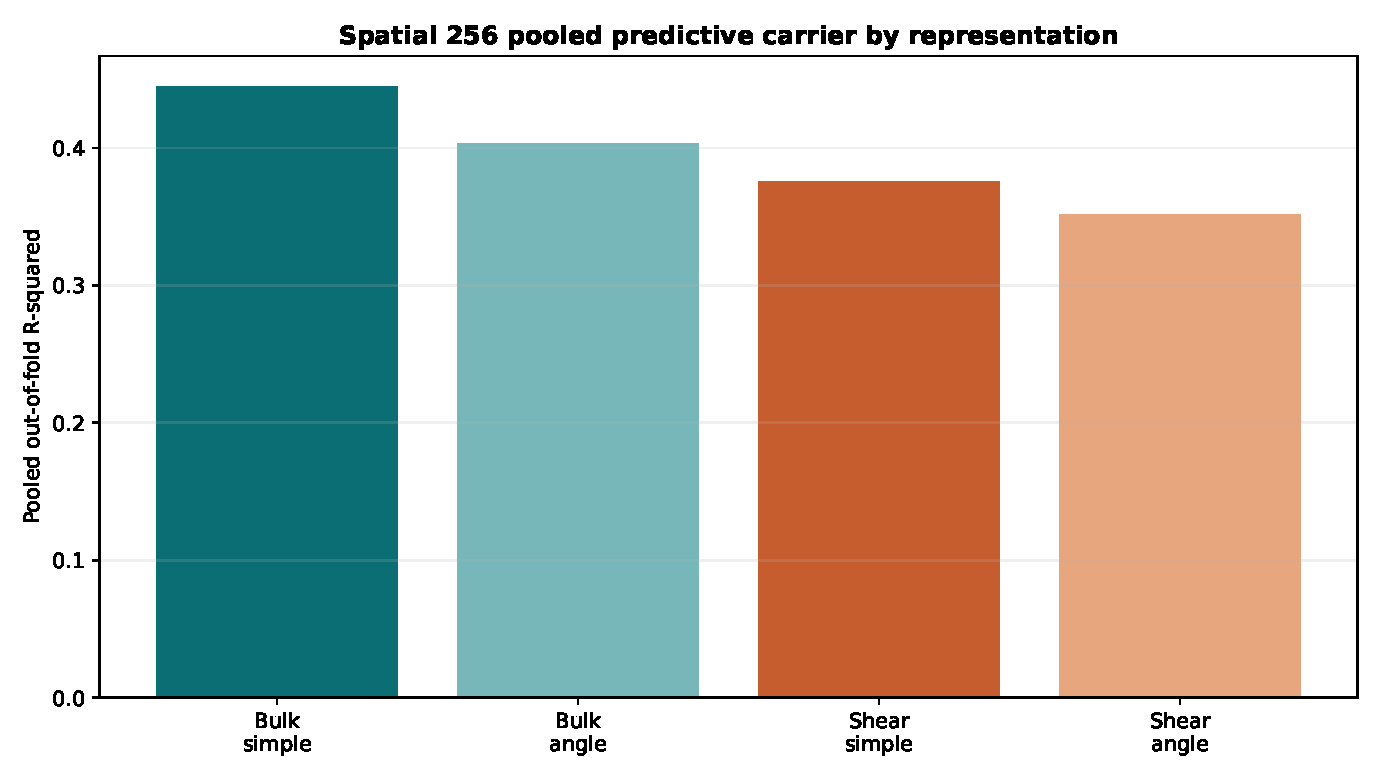
\includegraphics[width=0.90\textwidth]{figures/spatial_256_pooled_r2.pdf}
\caption{\textbf{SEALED AND REPLAYED LOCAL EVIDENCE.} Pooled out-of-fold
carrier performance for the two representations and targets.}
\end{figure}

\section{Why the angle summary failed to persist}

The execution architecture passed; the hypothesis did not. The diagnostic
identified three constraints.

\begin{enumerate}
\item The ascending-JID cohort and contiguous folds are deterministic and
result-blind, but not chemistry-stratified. They test persistence across fixed
blocks, not chemical transfer.
\item Six global histogram bins heavily compress local angular environments.
Different structures can therefore map to similar angle summaries.
\item The density-normalised bins obey an effectively fixed-sum closure
constraint. The simple standardised design condition number is
18.24; the angle
matrix reaches approximately $3.75\times10^{15}$ because one added direction
is redundant. Post-hoc standardisation did not restore the angle advantage.
\end{enumerate}

\begin{figure}[H]
\centering
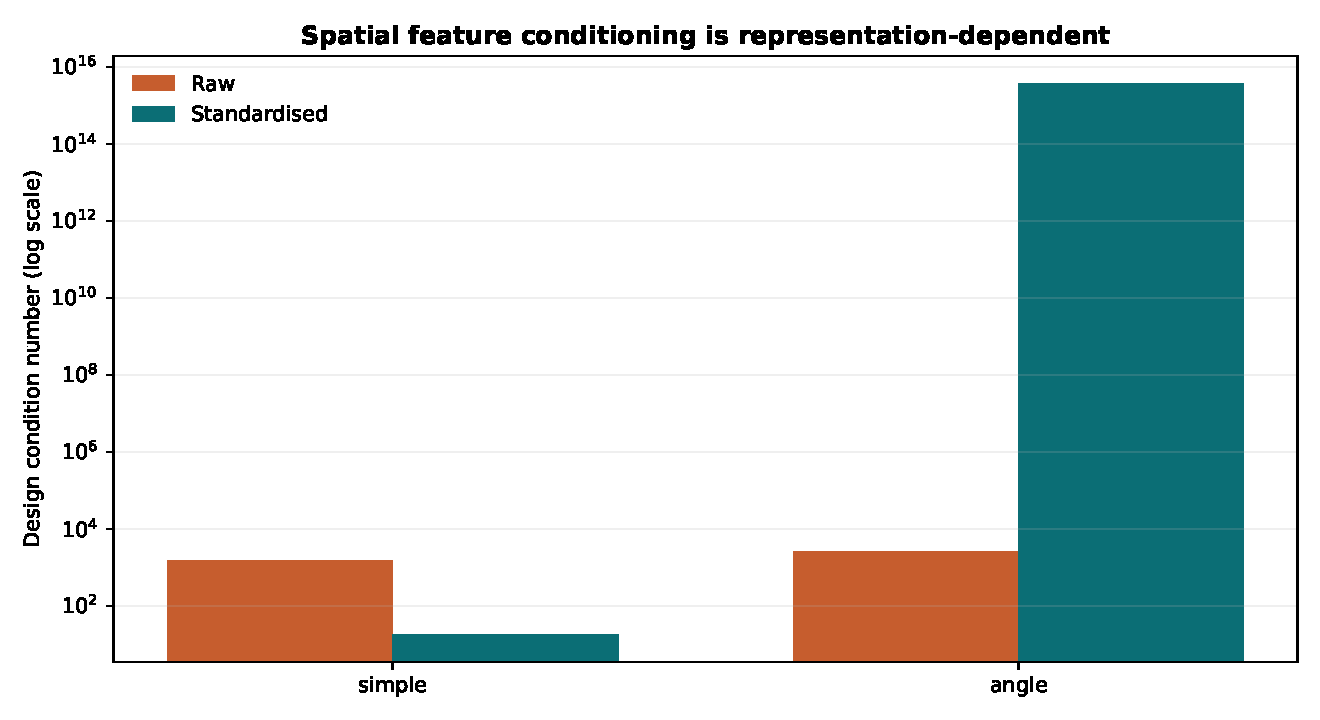
\includegraphics[width=0.88\textwidth]{figures/spatial_256_feature_conditioning.pdf}
\caption{\textbf{POST-HOC DIAGNOSTIC.} Raw and standardised design condition
numbers. This diagnostic explains a representation limitation but does not
replace the sealed protocol result.}
\end{figure}

\section{Decision}

\begin{center}
\hold{} \texttt{512 NOT AUTOMATICALLY ADMITTED}
\end{center}

The next experiment should not merely increase the same sample rule. It should
predeclare and freeze chemistry-aware memberships, remove the histogram closure
redundancy, include a sham representation-expansion control, and test whether a
less compressed angular representation earns its added cost. Only then should a
512-material stage be reconsidered.

\section{Claim boundary}

Supported: bounded local evidence that this repaired six-bin angle summary does
not provide a persistent advantage over the simple graph summary for bulk or
shear across the declared 256-material four-fold Ridge study.

Not supported: general inferiority of angular information, GNN conclusions,
defect physics, materials recommendation, physical validation or external
validation.


% CHAPTER 7A
% Structural/electrostatic DOE and live confirmation queue
% =========================================================

\chapter[Spatial DOE and Confirmation]{Spatial GIL:\ Structural DOE, Confirmation and Exact Replay}

\begin{center}
\fbox{\begin{minipage}{0.91\textwidth}
\textbf{Question.} Which structural information persists after matched controls, population changes, and exact replay?\\
\textbf{Comparison.} A 32-configuration factorial study isolated representation blocks; V0.6.1 then tested bulk metric geometry and shear polarity across continuity and zero chemical-system-overlap views.\\
\textbf{Result.} Bulk metric geometry passed both views; shear polarity passed the chemical-system view but failed the frozen continuity threshold. All 927,361 replayed numeric cells matched exactly.\\
\textbf{Decision.} Confirm compact metric geometry for this bulk route; retain shear polarity as conditional.\\
\textbf{Boundary.} Frozen 256-material Ridge study only; no 512-material, GNN, causal, or physical-qualification authority.
\end{minipage}}
\end{center}


\section{Why decomposition followed persistence failure}
The 64-material predecessor suggested an angle-aware advantage. At 256 materials the
six-bin angular summary failed to retain a persistent benefit. The correct response was
not immediate GNN escalation but a controlled 32-configuration decomposition of
coordination, continuous metric geometry and polarity proxies.

\section{V0.5 representation DOE}
The factorial study identified continuous metric geometry as the strongest compact
block: its mean R2 effect was +0.3503 for bulk and +0.2688 for shear. Coordination was
harmful, generic angular geometry was harmful or unstable, polarity was conditional,
and the full 43-feature representation underperformed selected smaller configurations.
These were block-level results, not proof of individual-feature mechanism.

\section{V0.6.1 confirmation contract}
The successor froze 256 materials, Ridge, two targets, continuity and zero
chemical-system-overlap views, four folds, nine configurations, matched shams and
paired target-permutation nulls. It comprised 144 valid and 432 null units. Views could
not repair each other by pooling.

\section{Final measured and replayed result}
Fresh and replay executions each sealed 576/576 units. All 1,728 corresponding output
pairs were byte-identical; 927,361 numeric cells matched exactly with maximum
difference zero; semantic metadata and plan identity passed. Controls passed with
maximum delta $2.331\times10^{-12}$ against $10^{-8}$. accepted evidence memory was disabled with zero
promotions.

Bulk metric geometry exceeded BASE by +0.4855 R2 under zero chemical-system overlap
and +0.4778 under continuity, exceeded matched shams by +0.5157 and +0.5145, and was
positive in 4/4 folds in both views. It therefore confirmed. Shear polarity over metric
geometry passed the grouped view (+0.0453; 4/4 folds) but failed continuity (+0.0123
against +0.02; 3/4 folds). It remains conditional.

\begin{governingrule}[Final spatial result]
More representation is not automatically better representation. Metric geometry
survived confirmation and exact replay; the stronger universal polarity claim did not.
\end{governingrule}

\section{Claim boundary}
The result is measured and controller-replayed locally for the frozen cohort, model,
folds, nulls and controls. It is not external validation, universal mechanism, 512-
material authority, GNN superiority, physical qualification or deployment permission.

\chapter{Three-Paper Decomposition and Research Questions}
\label{ch:publication-map}

The monograph is the synthesis object. It should not be submitted unchanged as
three overlapping articles. The publication programme separates three claims
that can be reviewed and falsified independently.

\begin{longtable}{p{0.20\textwidth}p{0.25\textwidth}p{0.28\textwidth}p{0.19\textwidth}}
\toprule
Article & Primary question & Decisive evidence & Excluded claim \\
\midrule
\endfirsthead
\toprule
Article & Primary question & Decisive evidence & Excluded claim \\
\midrule
\endhead
Paper 1: Importance Is Not Necessity & Do fitted rankings agree with retrained
removal consequences? & Matbench V0.3 sealed fresh, JARVIS bounded removal, and
Spatial V0.5 block interventions & No external replication; no universal
causal descriptor hierarchy \\
Paper 2: Better Than Null Is Not Yet Useful & Does a route satisfy both null
separation and absolute/transfer viability? & JARVIS, held MP elasticity,
Matbench task-native metrics, and Spatial split challenge & No invented null
$R^2$; no external validation \\
Paper 3: Available Evidence Is Not Engineering Authority & Can evidence be admitted, replayed, and
kept outside accepted memory when unsupported? & MP no-fit admissibility,
recovery-controlled JARVIS and Spatial replay, zero-promotion evidence-memory controls & No
database-wide corruption claim; no enterprise compliance claim \\
\bottomrule
\end{longtable}

\section{Open successors retained without result leakage}

\begin{itemize}
\item \textbf{Matbench V0.3 repeat:} completed under a separate execution identity;
65,740 compared numeric cells were exactly equal.
\item \textbf{Spatial GIL V0.6.1:} fresh and replay executions each sealed 576/576 units; exact replay retained bulk geometry PASS and shear polarity cross-view FAIL.
\item \textbf{MP tensor/method admission:} held until tensor-bearing evidence,
method receipts, domain review, and frozen cohort membership exist.
\item \textbf{Public research compendium:} sanitised papers, evidence summaries,
reference sources and contract boundaries prepared for archival deposit.
\end{itemize}

The queue is operational context, not a fourth evidence class. Every paper must
be updated only after a queued item seals and its claims are adjudicated.


\chapter{What Changed During the Programme}



\label{chap:programme-evolution}

\section{Programme-level synthesis}

Across the programme, the recurring failure mode was substitution between
evidence objects: fitted use for retrained dependence, null separation for
viability, availability for admission, replay for authority, or narrative
memory for accepted scientific state. Geatomica therefore treats evidence
as a stateful object whose authority increases only through explicit
transitions.

\begin{governingrule}[Authority inheritance]
A weaker state does not inherit the authority of a stronger one merely
because both occur in the same workflow.
\end{governingrule}





\section{The framework was not the starting point}



It is possible to read the completed architecture backwards and assume

that Geatomica began as a fully designed assurance framework.



It did not.



The programme began with a materials question:



\begin{quote}



Can a smaller set of governing descriptors recover enough material

behaviour to reduce modelling complexity without abandoning the

underlying physics?



\end{quote}



The later concepts of admission,

viability,

replay,

authority

and governance emerged because the original question repeatedly met

evidence that could not be interpreted safely through ordinary

single-score workflows.



The architecture is therefore best understood as the accumulated

response to experimental failure.



Each layer exists because an earlier layer proved insufficient.





\section{First transition: from descriptor discovery to descriptor stability}



The first ambition was descriptor discovery.



The programme sought compact relationships among:



\begin{itemize}



\item

composition;



\item

electronic state;



\item

energetic organisation;



\item

structure;



\item

packing;



\item

mechanical response.



\end{itemize}



Initial models produced feature rankings.



Those rankings were promising,

but they were conditional.



Changing the model family,

population scale

or split geometry altered the apparent descriptor account.



The first transition was therefore:



\begin{equation}
\text{descriptor discovery}
\rightarrow
\text{descriptor stability}.
\end{equation}



The scientific question changed from:



\begin{quote}



Which descriptors rank highest?



\end{quote}



to:



\begin{quote}



Which descriptor relations remain difficult to remove when the

modelling route changes?



\end{quote}





\section{Second transition: from stability to retrained dependence}



Stability across seeds or perturbations did not establish that the

descriptor was load-bearing.



The bounded JARVIS Extra Trees removal lane showed why, while the sealed Matbench fresh and repeat executions expose a large, exactly repeated fitted-importance versus retrained-removal disagreement.



A fitted route can rank a descriptor highly while a retrained route reallocates signal through correlated alternatives. The Matbench result is measured and repeated within the frozen same-environment protocol; mechanism and external replication remain unresolved.



The second transition was:



\begin{equation}
\text{stability}
\rightarrow
\text{retrained-dependence testing}.
\end{equation}



The question changed from:



\begin{quote}



Does this descriptor keep appearing?



\end{quote}



to:



\begin{quote}



What happens when this descriptor is made unavailable and the model is

allowed to reconstruct the problem?



\end{quote}





\section{Third transition: from signal to viability}



The Materials Project elasticity route exposed a different weakness.



A model could beat its paired null and still remain worse than

prediction of the mean.



The existence of non-random signal did not establish practical model

usefulness.



The third transition was:



\begin{equation}
\text{signal detection}
\rightarrow
\text{model viability}.
\end{equation}



The question changed from:



\begin{quote}



Did the model learn more than nonsense?



\end{quote}



to:



\begin{quote}



Did the model learn enough to justify interpretation?



\end{quote}





\section{Fourth transition: from available data to admissible evidence}



The raw Materials Project elastic population showed that a respected

database can expose values that require context before modelling.



The fourth transition was:



\begin{equation}
\text{data availability}
\rightarrow
\text{scientific admission}.
\end{equation}



The question changed from:



\begin{quote}



Is the target field populated?



\end{quote}



to:



\begin{quote}



Do the source identity,

units,

method,

sign

and physical bounds support the claim being requested?



\end{quote}





\section{Fifth transition: from repeatability to reproducibility contracts}



The JARVIS replay reproduced all compared numerical cells within the

frozen tolerance while failing raw-byte identity.



The Materials Project replay preserved scientific ordering while

failing the strict elastic numerical contract.



The fifth transition was:



\begin{equation}
\text{repeatability}
\rightarrow
\text{multi-contract reproducibility}.
\end{equation}



The question changed from:



\begin{quote}



Did the run happen again?



\end{quote}



to:



\begin{quote}



Which parts of the run were reproduced:

plan,

semantics,

numbers,

ordering

or bytes?



\end{quote}





\section{Sixth transition: from successful execution to recoverable science}



Long-running programmes were interrupted.



A normal modelling script would often restart from the beginning or

continue from an informal partial state.



The recovery controller instead used complete scientific units,

expected-output contracts

and verified checkpoints.



The sixth transition was:



\begin{equation}
\text{completed execution}
\rightarrow
\text{recoverable execution}.
\end{equation}



The question changed from:



\begin{quote}



Can this experiment finish?



\end{quote}



to:



\begin{quote}



Can this experiment survive interruption without changing what counts

as accepted evidence?



\end{quote}





\section{Seventh transition: from evidence to authority}



The programme eventually contained several valid but incompatible

evidence states:



\begin{itemize}



\item

strong prediction with replaceable descriptors;



\item

positive null separation with negative absolute performance;



\item

source availability without physical admissibility;



\item

scientific recurrence without strict numerical replay;



\item

numerical replay without byte identity;



\item

cross-source recurrence without matched-material transfer.



\end{itemize}



No single metric could represent these states honestly.



The seventh transition was:



\begin{equation}
\text{evidence}
\rightarrow
\text{bounded authority}.
\end{equation}



The final question became:



\begin{quote}



What decision,

if any,

does this exact combination of evidence permit?



\end{quote}





\begin{figure}[H]



\centering



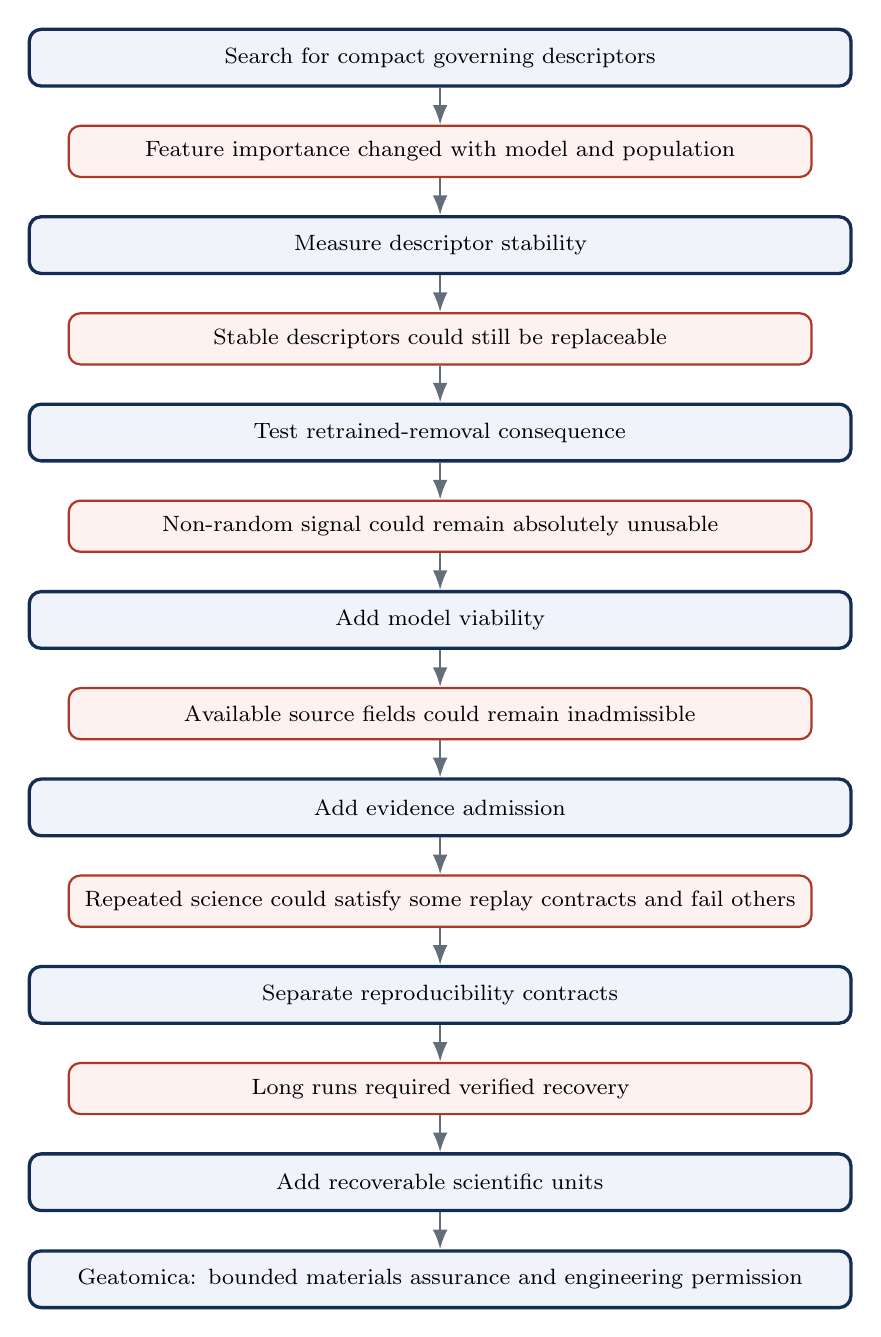
\begin{tikzpicture}[node distance=4.7mm, every node/.style={ font=\footnotesize, align=center }, stage/.style={ draw=geoBlue, very thick, rounded corners=1.5mm, fill=geoLight, text width=10.2cm, minimum height=0.72cm }, finding/.style={ draw=geoRust, thick, rounded corners=1.5mm, fill=geoRedLight, text width=9.2cm, minimum height=0.65cm }, final/.style={ draw=geoGreen, very thick, rounded corners=1.5mm, fill=geoGreenLight, text width=10.2cm, minimum height=0.78cm }]
\node[stage] (s1) {
    Search for compact governing descriptors
};
\node[finding, below=of s1] (f1) {
    Feature importance changed with model and population
};
\node[stage, below=of f1] (s2) {
    Measure descriptor stability
};
\node[finding, below=of s2] (f2) {
    Stable descriptors could still be replaceable
};
\node[stage, below=of f2] (s3) {
    Test retrained-removal consequence
};
\node[finding, below=of s3] (f3) {
    Non-random signal could remain absolutely unusable
};
\node[stage, below=of f3] (s4) {
    Add model viability
};
\node[finding, below=of s4] (f4) {
    Available source fields could remain inadmissible
};
\node[stage, below=of f4] (s5) {
    Add evidence admission
};
\node[finding, below=of s5] (f5) {
    Repeated science could satisfy some replay contracts and fail others
};
\node[stage, below=of f5] (s6) {
    Separate reproducibility contracts
};
\node[finding, below=of s6] (f6) {
    Long runs required verified recovery
};
\node[stage, below=of f6] (s7) {
    Add recoverable scientific units
};
\node[stage, below=of s7] (term_end) {
    Geatomica:
    bounded materials assurance and engineering permission
};
\foreach \a/\b in {
    s1/f1,
    f1/s2,
    s2/f2,
    f2/s3,
    s3/f3,
    f3/s4,
    s4/f4,
    f4/s5,
    s5/f5,
    f5/s6,
    s6/f6,
    f6/s7,
    s7/term_end}
{
    \draw[
        -{Latex[length=2.5mm]},
        thick,
        color=geoGrey
    ]
    (\a) -- (\b);
}
\end{tikzpicture}



\caption{How the Geatomica programme changed. Each new layer was introduced after the preceding evidence object failed to support the decision being requested.}



\label{fig:programme-evolution-full}



\end{figure}





\section{The unifying result: materials assurance}



The completed programme is not best described as:



\begin{itemize}



\item

a feature-selection method;



\item

a new regressor;



\item

a database-cleaning script;



\item

a reproducibility tool;



\item

a software-governance framework.



\end{itemize}



Each of those descriptions captures part of the work.



None captures the whole programme.



The unifying research object is

\term{materials assurance}.



Materials assurance asks:



\begin{quote}



When does a result extracted from materials data deserve to influence

an engineering decision?



\end{quote}



That question sits between:



\begin{equation}
\text{materials}
\rightarrow
\text{evidence}
\rightarrow
\text{decision}.
\end{equation}



The computational architecture is instrumentation around that chain.





\section{Why this is not simply uncertainty quantification}



Uncertainty quantification commonly estimates uncertainty in:



\begin{itemize}



\item

predictions;



\item

parameters;



\item

data;



\item

model ensembles;



\item

distribution shift.



\end{itemize}



Geatomica overlaps with these concerns.



Its focus is different.



The programme asks whether different evidence objects agree on the

permission being requested.



A model may show low predictive uncertainty while:



\begin{itemize}



\item

using an inadmissible source population;



\item

depending on a replaceable descriptor;



\item

failing an applicability-domain transfer;



\item

failing strict replay;



\item

remaining absolutely worse than the mean.



\end{itemize}



Uncertainty estimates remain valuable.



They do not replace evidence adjudication.





\section{Why this is not simply applicability domain}



An applicability domain asks where a model's predictions are expected

to remain reliable.



Descriptor authority asks an additional question:



\begin{quote}



Does the explanation remain reliable enough to support the same

engineering interpretation within that domain?



\end{quote}



A model can predict well inside its applicability domain while using

different correlated routes across learners.



Prediction domain and explanation domain are related.



They are not identical.





\section{Why this is not simply feature stability}



Feature stability asks whether a selected feature or ranking recurs

across repeated fits or perturbed samples.



Descriptor authority also requires attention to:



\begin{itemize}



\item

absolute model viability;



\item

negative controls;



\item

source admission;



\item

retrained removal;



\item

population transfer;



\item

replay;



\item

the action being requested.



\end{itemize}



A stable feature inside a failed carrier model does not gain

engineering authority through repetition alone.





\section{Why adverse results strengthened the programme}



A conventional publication strategy might have removed or minimised

the routes that did not produce clean positive results.



That would have removed the evidence that most clearly demonstrates

the purpose of the programme.



The adverse results established that Geatomica could:



\begin{itemize}



\item

detect a defect in its own aggregation logic;



\item

preserve the original output;



\item

introduce a successor rule without rewriting history;



\item

hold a respected source field before physical interpretation;



\item

complete a replay while refusing strict numerical equivalence;



\item

retain useful energetic and electronic evidence alongside held

elasticity;



\item

return a smaller honest answer rather than one inflated headline.



\end{itemize}



These are not side effects.



They are the empirical basis of the assurance claim.





\begin{governingrule}



A scientific assurance system is not demonstrated only by the evidence

it promotes.



It is demonstrated by the evidence it refuses to overstate.



\end{governingrule}





\section{The current research object}



The final Geatomica research object can be stated as:



\begin{quote}



A governed materials-informatics instrument that measures how

predictive relationships,

descriptor explanations

and source evidence respond to declared changes,

then issues only the bounded engineering permission supported by the

surviving evidence.



\end{quote}



Its principal outputs are:



\begin{itemize}



\item

predictive carrier-signal evidence;



\item

descriptor-response barcodes;



\item

retrained-removal consequence results;



\item

source-admission states;



\item

model-viability states;



\item

population-transfer boundaries;



\item

replay contracts;



\item

recovery receipts;



\item

bounded engineering permissions;



\item

explicit refusals.



\end{itemize}





\section{What remains unresolved}



The programme has not yet completed its original scientific ambition.



It has not produced a validated universal reduced descriptor spine.



It has instead constructed the assurance conditions under which such a

spine could be tested honestly.



The remaining questions include:



\begin{itemize}



\item

Do any descriptor combinations persist across additional independent

sources?



\item

Can electronic descriptors such as band gap or density-of-states

quantities remain informative after controlling for material class?



\item

Do spatial and graph representations preserve the same descriptor

zones?



\item

Can reduced descriptor sets guide new DFT calculations more

efficiently?



\item

Do the nominated relationships survive physical measurements?



\item

Can dynamic material transitions be modelled without importing static

feature logic into time-dependent systems?



\item

How should authority thresholds change with engineering consequence?



\end{itemize}



The assurance framework is therefore not the end of Geatomica.



It is the experimental substrate required for the next materials

questions.





\section{Chapter conclusion}



The programme began with a search for compact governing descriptors.



The experiments forced that question to widen.



Feature importance was not enough.



Stability was not enough.



Null separation was not enough.



Source availability was not enough.



One completed run was not enough.



Even successful replay was not one indivisible state.



The resulting framework did not emerge because more terminology was

desired.



It emerged because each previous evidence object failed to support the

engineering permission being asked of it.



Geatomica is therefore best understood as a materials-assurance

programme.



Its purpose is not to make every model trustworthy.



Its purpose is to make the boundary of trust measurable.





% ============================================================

% END OF PART 3

%

% NEXT BLOCK:

%

% CHAPTER 8

% Practical Materials-Engineering Decisions

%

% CHAPTER 9

% Runtime, Recovery and Evidence Lineage

%

% CHAPTER 10

% Governance and Claim Authority

% ============================================================

% ============================================================

% PART 4

%

% CHAPTER 8

% Practical Materials-Engineering Decisions

%

% CHAPTER 9

% Runtime, Recovery and Evidence Lineage

%

% CHAPTER 10

% Governance and Claim Authority

% ============================================================





% ============================================================

% CHAPTER 8

% ============================================================



\chapter[Beyond Materials ML]{Beyond Materials ML:\\ Engineering Transfer and Bounded Design Studies}

Materials ML exposed the evidence problem in a controlled scientific setting. It showed that a model could appear important, non-null, reproducible, or complete without earning the stronger interpretation being asked of it. The engineering studies exposed the same control problem at the action boundary: geometry changes broke transfer of thermal evidence, invalid state transitions remained invalid even when numerically evaluable, and fault containment improved while thermal performance degraded.

\begin{center}\small\bfseries
MATERIALS ML\\
What does the model or evidence actually support?\\
$\downarrow$\\
importance / viability / replay distinctions\\
$\downarrow$\\
GENERAL COMPUTATIONAL ENGINEERING\\
What may the result legitimately change next?
\end{center}

The engineering cases show transferable control behaviour across three local computational engineering studies. They do not constitute retrospective validation of the complete modern Systemica architecture, physical validation, external validation, or industrial deployment.

\section{Three local engineering witnesses}

\begin{longtable}{L{0.13\textwidth}L{0.18\textwidth}L{0.29\textwidth}L{0.29\textwidth}}
\toprule
\textbf{Case} & \textbf{Starting decision} & \textbf{Consequential correction or failure} & \textbf{Bounded outcome and lineage}\\
\midrule
Furnace viewport & Whether a thermal-interface concept was mature enough to fabricate or test. & Correcting 350--375 mm to 35--40 mm broke transfer of an inherited 59.2~$^\circ$C result. Active cooling added a dependency and failure route. & Thermal screen plus uncertainty/fault scenarios led to a guarded opaque thermal-interface coupon. Fabrication and furnace operation were not authorised. Later services formalised case identity, predecessor transfer, failure retention, and bounded action.\\
Dual tank & Whether a reserve, feeder, recovery, and return topology could advance. & Fresh reserve, live feeder/recovery, and returned or consumed states had to remain distinct. Forbidden return transitions were rejected even when a numerical route could be evaluated. & A low-pressure non-potable tracer rig was the next test; deployment was not authorised. Later services formalised typed state, topology, transition validity, and provenance.\\
Heat shield & Whether segmentation improved a thermal-flow protection concept. & Segmentation improved fault containment while degrading thermal performance. Blocked-cell and contained-leak cases remained visible rather than being averaged away. & Matched cold-flow and heated coupons were specified; qualification and flight readiness were not authorised. Later services formalised competing-objective and failure-case retention.\\
\bottomrule
\end{longtable}

Across the three studies, 13 candidate objects, five descendants, 116 scenarios, 9,150 parameter or uncertainty runs, and at least 9,380 model operations narrowed broad concepts to smaller falsifiable tests. The counts show bounded computational activity, not labour savings, physical qualification, or industrial validation.

\section{What was actually engineered and modelled}

The three engineering studies were bounded pre-experimental calculations, not architecture demonstrations wearing engineering labels. They began with physical design questions and ended with smaller physical tests.

\begin{longtable}{L{0.11\textwidth}L{0.19\textwidth}L{0.25\textwidth}L{0.23\textwidth}L{0.15\textwidth}}
\toprule
\textbf{Case} & \textbf{Physical object} & \textbf{Native model} & \textbf{Principal failure discovered} & \textbf{Bounded next test}\\\midrule
Furnace & High-temperature viewport/thermal interface & Deterministic dominant-path thermal screening with uncertainty and fault sweeps & Corrected geometry invalidated inherited evidence; cooling created a dependency; edge/frame transfer remained unresolved & Guarded opaque thermal-interface coupon\\
Dual tank & Reserve/feeder/recovery topology & Lumped flow/state model with typed topology and transition validation & Recovered water had been collapsed into reserve; invalid return routes remained possible & Low-pressure non-potable tracer rig\\
Heat shield & Segmented transpiration/fault-containment coupon & Transient cell thermal network with Darcy-style flow and topology/fault checks & Maximum nominal cooling and fault localisation diverged & Matched cold-flow/heated blocked/leak coupons\\
\bottomrule
\end{longtable}

These are bounded screening and pre-experimental engineering instruments, not physical validation of the proposed systems.

\subsection{Furnace thermal enclosure and viewport interface}
The engineered object was a brazing-furnace thermal enclosure and removable optical/thermal viewport interface intended to provide process visibility without allowing the optical path to dominate external heat transfer or compromise the surrounding thermal boundary. The corrected intended interface envelope was 35--40 mm, not the inherited 350--375 mm. The previously reported 59.2~$^\circ$C cold-side result was retained historically but refused for current design authority because it belonged to the wrong geometry identity.

The executed bounded model used deterministic dominant-path thermal-resistance screening, candidate-specific heat paths, six model/fault scenarios, 9,000 deterministic uncertainty samples, and 9,120 model operations. Variables included emissivity, hot-side boundary, contact resistance, wall depth, seal/interface assumptions, aperture, cooling-loss behaviour, and unresolved edge/frame transfer. F-A was a minimum-complexity single-pane control; F-B separated functions with a passive double-pane/cavity; F-C tested active cooling; F-A1 and F-B1 were descendants created after weaknesses appeared.

The second pane/cavity improved the declared central cold-side path, and a smaller aperture improved the pressure screen. Active cooling improved nominal temperature while adding a failure dependency. Variation across 35--40 mm did not remove the dominant optical path in this lightweight model, and edge/frame transfer remained unresolved. The engineering value was the conversion of an incorrectly inherited geometry and broad idea into traceable candidate families, quantified uncertainty, explicit failure dependencies, and a guarded coupon targeting the unresolved paths. It was not a validated final viewport.

\subsection{Dual-tank provenance and recovery topology}
The physical object was a multi-reservoir water distribution and recovery topology separating clean make-up reserve, live feeder/recovery flow, unused return, consumed water, and contained/rejected states while buffering demand. The correction made R the isolated new-source reserve and F the live feeder/recovery tank. Only declared unused return could pass a quality gate into F; consumed water exited; excess remained contained. Source provenance, age/residence, return history, and gate history were kept distinct because equal level or pressure does not imply equal reuse history.

The executed model combined lumped flow/state simulation, typed topology, candidate-specific transition validation, 26 scenarios, and 70 parameter cases. Forbidden routes were rejected before execution. W-B2 scored 33/35 under the exploratory screen; W-B4 was generated after W-B2 failed the peak criterion and scored 34/35. Its worst service-margin failure improved from $-0.266$ to $-0.090$ under those assumptions. These are not final sizing values.

The engineering contribution was correction of the physical state topology. Recirculation could recondition water without making it new-source water; capacity and provenance integrity remained different objectives. Final size, hygiene, pressure losses, water quality, and component ratings remain unresolved. The next action was a transparent low-pressure non-potable tracer rig measuring provenance, residence, and fault containment.

\subsection{Segmented transpiration heat-shield coupon}
The engineered object was a segmented porous/transpiration thermal-management ground coupon in which coolant delivery, thermal response, and cell-level fault containment were competing objectives. The model coupled a two-node-per-cell transient thermal network, Darcy-style permeability/restriction flow, structural topology, and transition/fault-route validation. It executed 84 scenarios and 80 parameter cases across six candidate/control objects, generated two descendants, and rejected four unsupported route classes.

Thermal nodes approximated coupon heat storage and transfer; restricted flow represented the porous delivery path; segmentation tested whether blockage or leakage remained local. H-A1, the monolithic route, carried the strongest nominal thermal signal with a temperature-reduction range of 175.3--389.5 K. H-B1, the segmented descendant, traded thermal response for isolation and maintenance information; its range included $-83.5$ to 245.4 K. Segmentation was therefore not a free improvement.

The model did not resolve pore-scale convection, choking or compressibility, external film formation, spectral radiation, oxidation, erosion or ablation, detailed contacts, or flight aerothermodynamics. Its value was to produce a falsifiable matched-coupon sequence: no-flow control, simple thermal/permeability route, segmented fault-isolation route, blocked-cell case, and contained-leak case. No qualification or flight readiness followed.

The technical contribution here is the design synthesis and engineering reduction demonstrated within the programme, not a claim of literature-level novelty for every physical mechanism.


\section{Architecture provenance}

\begin{figure}[H]
\centering
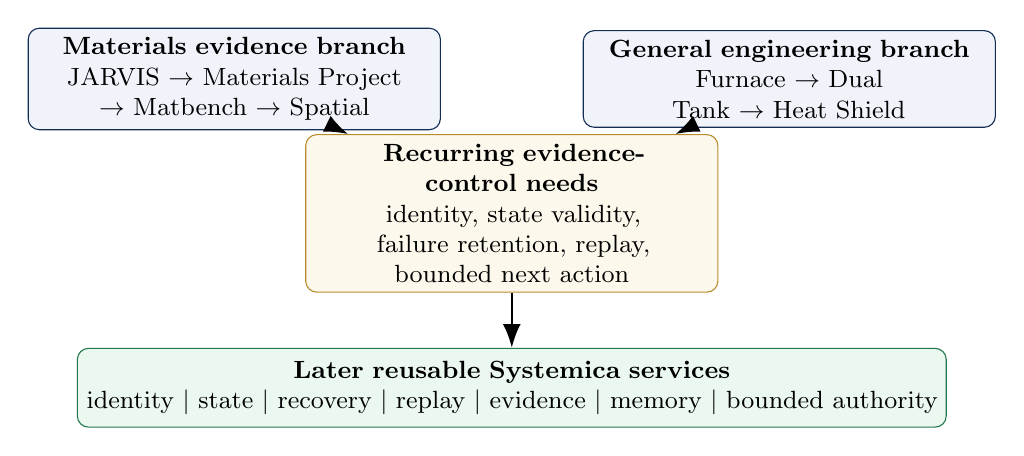
\begin{tikzpicture}[node distance=7mm, every node/.style={align=center,font=\small}, branch/.style={draw=geoBlue,rounded corners,fill=geoLight,text width=5.0cm,minimum height=1.0cm}, centre/.style={draw=geoGold,rounded corners,fill=geoGoldLight,text width=5.0cm,minimum height=1.0cm}, service/.style={draw=geoGreen,rounded corners,fill=geoGreenLight,text width=10.8cm,minimum height=1.0cm}]
\node[branch] (materials) {\textbf{Materials evidence branch}\\JARVIS $\rightarrow$ Materials Project $\rightarrow$ Matbench $\rightarrow$ Spatial};
\node[branch,right=18mm of materials] (engineering) {\textbf{General engineering branch}\\Furnace $\rightarrow$ Dual Tank $\rightarrow$ Heat Shield};
\node[centre,below=of $(materials)!0.5!(engineering)$] (logic) {\textbf{Recurring evidence-control needs}\\identity, state validity, failure retention, replay, bounded next action};
\node[service,below=of logic] (services) {\textbf{Later reusable Systemica services}\\identity $|$ state $|$ recovery $|$ replay $|$ evidence $|$ memory $|$ bounded authority};
\draw[-{Latex[length=3mm]},thick] (materials) -- (logic);
\draw[-{Latex[length=3mm]},thick] (engineering) -- (logic);
\draw[-{Latex[length=3mm]},thick] (logic) -- (services);
\end{tikzpicture}
\caption{Two evidence branches converged on recurring control needs. The later architecture abstracts those behaviours; it was not retrospectively present in full in the historical cases.}
\label{fig:architecture-provenance}
\end{figure}

Repeated behaviours observed across case-specific scientific and engineering workflows were progressively formalised into reusable execution, evidence, replay, memory, state, and bounded-authority services. Scientific-domain transfer remains unestablished beyond demonstrated materials semantics. Control-logic transfer has initial local evidence across materials ML/data analysis, thermal-interface design, fluid/state topology, and thermal-flow/fault-containment design.



\label{chap:engineering-decisions}





\section{Evidence becomes useful when it changes the next action}



The preceding chapters established that materials-model evidence can

separate into several distinct states.



A model can predict well while its explanation remains replaceable.



A relationship can recur across runs while failing under a harder

population split.



A populated source field can remain unresolved for physical

interpretation.



A model can beat a null while remaining worse than predicting the

mean.



A scientific pattern can recur while a stricter numerical replay

contract fails.



These distinctions become practically useful only when they alter what

an engineer does next.



The purpose of Geatomica is therefore not to add another explanatory

layer after prediction.



It is to place a decision boundary between a modelling result and the

engineering action that may follow from it.



That boundary asks:



\begin{quote}



What is the least expensive next action that remains scientifically

justified by the surviving evidence?



\end{quote}



The answer may be to continue using the current route.



It may be to escalate to a richer calculation or physical test.



It may be to request additional source information.



It may be to stop.





\begin{governingrule}



A model result should not acquire authority because it is available.



It should acquire only the authority required for the next justified

action.



\end{governingrule}





\section{The engineering decision ladder}



Materials development is already organised as a sequence of increasing

cost and commitment.



A typical progression may move through:



\begin{itemize}



\item

database search;



\item

composition-based screening;



\item

reduced tabular modelling;



\item

higher-fidelity electronic-structure calculation;



\item

thermodynamic or kinetic modelling;



\item

atomistic simulation;



\item

coupon manufacture;



\item

physical characterisation;



\item

component-scale testing;



\item

qualification.



\end{itemize}



Each stage consumes more time,

compute,

material,

specialist labour

or equipment access.



The value of a low-cost model is therefore not determined only by its

terminal accuracy.



Its value also depends on whether it helps decide where more expensive

work is worth doing.



Geatomica inserts an assurance step before escalation.





\begin{figure}[H]



\centering



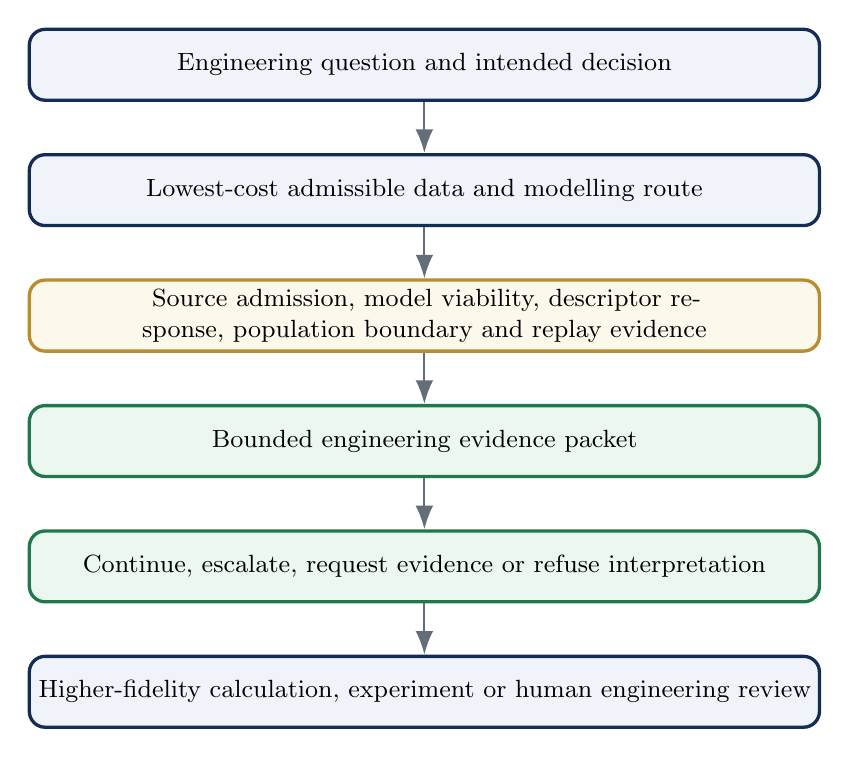
\begin{tikzpicture}[node distance=6.5mm, every node/.style={ font=\small, align=center }, stage/.style={ draw=geoBlue, very thick, rounded corners=2mm, fill=geoLight, text width=9.8cm, minimum height=0.9cm }, audit/.style={ draw=geoGold, very thick, rounded corners=2mm, fill=geoGoldLight, text width=9.8cm, minimum height=0.9cm }, decision/.style={ draw=geoGreen, very thick, rounded corners=2mm, fill=geoGreenLight, text width=9.8cm, minimum height=0.9cm }]
\node[stage] (question) {
    Engineering question and intended decision
};
\node[
    stage,
    below=of question
] (cheap) {
    Lowest-cost admissible data and modelling route
};
\node[
    audit,
    below=of cheap
] (audit) {
    Source admission,
    model viability,
    descriptor response,
    population boundary
    and replay evidence
};
\node[
    decision,
    below=of audit
] (packet) {
    Bounded engineering evidence packet
};
\node[
    decision,
    below=of packet
] (action) {
    Continue,
    escalate,
    request evidence
    or refuse interpretation
};
\node[
    stage,
    below=of action
] (higher_action) {
    Higher-fidelity calculation,
    experiment
    or human engineering review
};
\foreach \a/\b in {
    question/cheap,
    cheap/audit,
    audit/packet,
    packet/action,
    action/higher_action}
{
    \draw[
        -{Latex[length=3mm]},
        thick,
        color=geoGrey
    ]
    (\a) -- (\b);
}
\end{tikzpicture}



\caption{The engineering decision ladder. Geatomica sits between a low-cost modelling route and the next expensive action. Its purpose is not to prevent escalation, but to determine when escalation is justified and what uncertainty it must resolve.}



\label{fig:engineering-decision-ladder}



\end{figure}





The ladder is not a rigid universal workflow.



Different materials programmes begin and end at different stages.



A mature alloy family may already have extensive experimental history.



A novel composition may begin with sparse calculated evidence.



A process-development question may require kinetic or thermal models

rather than a property predictor.



The assurance principle remains the same:



\begin{equation}
\text{use the cheapest route that remains valid for the decision,}
\end{equation}



then escalate when the evidence boundary is reached.





\section{Continue, escalate, request evidence or refuse}



The practical output is not a binary label of

\emph{trusted}

or

\emph{untrusted}.



Four bounded outcomes are more useful.



\subsection{Continue}



The current route may continue when:



\begin{itemize}



\item

the source population is admissible for the intended claim;



\item

the model crosses both viability doors;



\item

the material candidate lies within the evidenced population boundary;



\item

the relevant descriptor account remains coherent under the declared

disturbances;



\item

the result satisfies the required replay contract;



\item

the requested action remains low consequence.



\end{itemize}



Continue does not mean universal acceptance.



It means that the current low-cost route remains suitable for the next

bounded step.





\subsection{Escalate}



Escalation is appropriate when useful signal exists,

but the current representation cannot support the requested decision.



Examples include:



\begin{itemize}



\item

row-random performance remains strong,

but the candidate lies in an unseen chemical system;



\item

bulk-modulus prediction remains coherent,

but shear behaviour is weak and directionality matters;



\item

composition descriptors perform well,

but the candidate's structure is uncertain;



\item

descriptor importance and retrained-removal consequence disagree;



\item

the model is viable,

but the intended action carries high consequence;



\item

the reduced route cannot resolve competing physical interpretations.



\end{itemize}



Escalation may involve:



\begin{itemize}



\item

a richer structural representation;



\item

graph or spatial modelling;



\item

additional DFT calculations;



\item

CALPHAD or kinetic modelling;



\item

molecular dynamics;



\item

finite-element analysis;



\item

physical characterisation;



\item

targeted mechanical testing.



\end{itemize}





\subsection{Request additional evidence}



Some routes should pause before either continuing or escalating.



This occurs when the missing object is not a richer model,

but a clearer source.



Examples include:



\begin{itemize}



\item

uncertain units;



\item

missing method provenance;



\item

unresolved sign conventions;



\item

unclear tensor-to-scalar reduction;



\item

ambiguous material identity;



\item

duplicate or conflicting records;



\item

missing process history;



\item

incomplete environmental conditions.



\end{itemize}



A more complex learner cannot resolve a missing scientific definition.





\subsection{Refuse interpretation}



Refusal is appropriate when:



\begin{itemize}



\item

the source is inadmissible for the requested claim;



\item

the model fails both viability doors;



\item

the candidate is materially outside the evidenced domain;



\item

the requested action exceeds the claim ceiling;



\item

the execution or replay evidence is incomplete;



\item

the result depends on a known leakage route;



\item

a failed gate is being repaired only through narrative reinterpretation.



\end{itemize}



Refusal does not mean that the material is unsuitable.



It means that the present evidence cannot justify the requested

conclusion.





\begin{table}[H]



\centering



\caption{Engineering actions associated with bounded evidence states.}



\label{tab:engineering-actions}



\begin{tabularx}{\textwidth}{L{0.18\textwidth}
    Y
    Y
}
\toprule
\textbf{Action}
&
\textbf{Evidence condition}
&
\textbf{Typical next step}
\\
\midrule
Continue
&
Admissible source,
viable model,
bounded transfer
and adequate replay for a low-consequence action.
&
Retain the reduced route for screening or exploratory interpretation.
\\
\addlinespace
Escalate
&
Useful signal exists,
but representation,
domain
or consequence exceeds the present evidence.
&
Run higher-fidelity simulation,
collect richer descriptors
or perform a targeted experiment.
\\
\addlinespace
Request evidence
&
The main uncertainty lies in source meaning,
provenance
or missing context.
&
Resolve units,
method,
identity,
tensor meaning
or process history before further modelling.
\\
\addlinespace
Refuse
&
An earlier gate fails or the requested claim exceeds the evidence
ceiling.
&
Do not promote the model result into engineering interpretation.
\\
\bottomrule
\end{tabularx}



\end{table}





\section{The bounded engineering evidence packet}



A conventional machine-learning result often ends with:



\begin{itemize}



\item

one performance score;



\item

one ranked feature list;



\item

one selected model.



\end{itemize}



An engineer needs a different object.



The Geatomica evidence packet is intended to include:



\begin{enumerate}



\item

\term{Decision statement}



What engineering question is being asked?



\item

\term{Source statement}



Which source,

version,

population

and admission rules were used?



\item

\term{Model statement}



Which representation,

learner,

split

and preprocessing route produced the prediction?



\item

\term{Viability statement}



Did the model cross both the absolute and relative evidence doors?



\item

\term{Population boundary}



Which compositions,

chemical systems,

structures

or operating conditions are covered?



\item

\term{Descriptor response}



Which relationships recur,

which are fragile

and which are replaceable?



\item

\term{Replay state}



Which plan,

semantic,

numerical

and byte contracts passed?



\item

\term{Known defects and unresolved assumptions}



What remains uncertain or held?



\item

\term{Permitted action}



What may the engineer do next?



\item

\term{Prohibited interpretation}



What must not be inferred from the result?



\end{enumerate}





\begin{figure}[H]



\centering



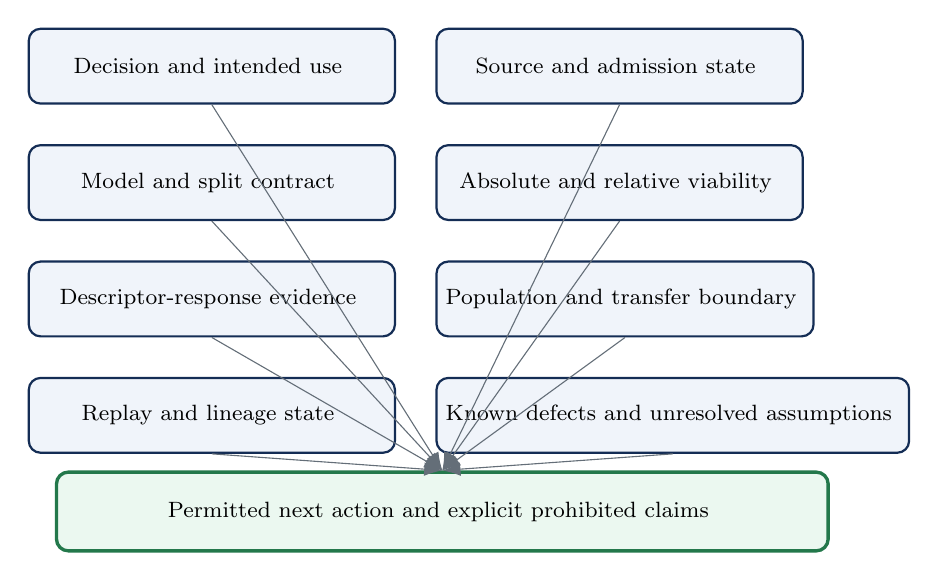
\begin{tikzpicture}[node distance=5mm and 5mm, every node/.style={ font=\footnotesize, align=center }, packet/.style={ draw=geoBlue, thick, rounded corners=1.5mm, fill=geoLight, minimum width=4.65cm, minimum height=0.95cm }, outcome/.style={ draw=geoGreen, very thick, rounded corners=1.5mm, fill=geoGreenLight, minimum width=9.8cm, minimum height=1.0cm }]
\node[packet] (decision) {
    Decision and intended use
};
\node[
    packet,
    right=of decision
] (source) {
    Source and admission state
};
\node[
    packet,
    below=of decision
] (model) {
    Model and split contract
};
\node[
    packet,
    right=of model
] (viability) {
    Absolute and relative viability
};
\node[
    packet,
    below=of model
] (descriptor) {
    Descriptor-response evidence
};
\node[
    packet,
    right=of descriptor
] (domain) {
    Population and transfer boundary
};
\node[
    packet,
    below=of descriptor
] (replay) {
    Replay and lineage state
};
\node[
    packet,
    right=of replay
] (defects) {
    Known defects and unresolved assumptions
};
\node[
    outcome,
    below=7mm of $(replay)!0.5!(defects)$
] (permission) {
    Permitted next action and explicit prohibited claims
};
\foreach \a in {decision, source, model, viability, descriptor, domain, replay, defects}
{
    \draw[-{Latex[length=2.3mm]}, thin, color=geoGrey] (\a.south) -- (permission.north);
}
\end{tikzpicture}

\caption{Conceptual bounded engineering evidence packet.}
\label{fig:evidence-packet}

\end{figure}

\section{Bounded screening of elastic response}

Consider a hypothetical materials-screening task. An engineer wants to identify candidates likely to retain useful bulk stiffness within a defined chemical family.

A conventional route may:
\begin{enumerate}
\item train a property model;
\item rank candidate materials;
\item select the top-scoring compounds.
\end{enumerate}

A Geatomica route asks additional questions.

\subsection{Source admission}
Are the elastic targets physically interpretable under the available units, method and bound definitions? If not, the route stops before fitting authority is granted.

\subsection{Model viability}
Does the model satisfy $R^2>0$ and $S>0$? If only the null-separation door passes, the result may support diagnosis but not screening.

\subsection{Population boundary}
Does the candidate lie within a represented composition or chemical system? A row-random score cannot authorise unseen-chemistry use.

\subsection{Descriptor response}
Do density and volume-per-atom relationships recur across models and disturbances? Are they difficult to replace, or do correlated descriptors reconstruct the route?

\subsection{Engineering action}
A candidate may then be retained for low-cost preliminary screening, escalated to a structural or graph model, nominated for a fresh DFT calculation, held pending source resolution, or refused if outside the evidenced domain.

The output is not: "This material has a high predicted modulus." It is closer to: "This candidate ranks favourably within the declared chemical region under a viable bulk-modulus model. Packing-related descriptors recur across the tested routes, but the candidate lies near the composition-domain boundary. Use the result to nominate a higher-fidelity calculation. Do not use it to remove mechanical testing or claim unseen-system transfer."

\section{Cost-aware materials development}
The direct value of materials assurance lies partly in avoiding misallocated effort. A low-cost audit may identify that a candidate lies outside the training domain, the selected target is inadmissible, the model is better than a null but absolutely unusable, a feature interpretation is replaceable, a result fails replay, or a supposedly reduced descriptor set loses critical behaviour.

Each early detection can prevent more expensive work from being commissioned on a weak foundation. However, the monograph does not yet report a controlled industrial cost-saving trial. Any financial example remains illustrative until measured against a real engineering programme.

\begin{claimboundary}[Cost claim boundary]
The present evidence supports the proposition that earlier refusal and better escalation can reduce wasted work in principle. It does not yet quantify industrial savings, return on investment or avoided experimental cost.
\end{claimboundary}

\section{Relationship to established materials tools}
Geatomica does not replace density-functional theory, CALPHAD, molecular dynamics, phase-field modelling, finite-element analysis, microscopy, diffraction, mechanical testing or qualification procedures. These methods answer different questions.

Geatomica helps decide which route is justified, which candidates deserve escalation, which assumptions require resolution, which evidence may be used only exploratorily, and which interpretation must stop. It is an assurance layer around the transition from low-cost evidence to higher-cost engineering action.

\section{Human authority}
The final decision remains human. This is not only a safety statement; it follows from the scientific structure of the problem. The model does not possess complete process history, full economic context, manufacturing constraints, regulatory obligations, test availability, programme priorities, or responsibility for the consequence.

The system can structure evidence and limit unsupported promotion. It cannot replace the engineer who holds the complete decision context.

\begin{governingrule}
Geatomica may nominate, bound, escalate, hold or refuse. It does not own the engineering decision.
\end{governingrule}

\section{Chapter conclusion}
The practical contribution of Geatomica is not a new material property prediction by itself. It is a decision structure around prediction. The audit determines whether the source can be interpreted, whether the model is viable, whether the explanation persists, where the population boundary lies, whether the result can be replayed, and what action the evidence supports.

This converts model evaluation into an engineering workflow. The next question is whether the evidence packet itself can be trusted to survive long execution, interruption, comparison and later inspection. That requires runtime, recovery and lineage.


% ============================================================
% CHAPTER 9
% ============================================================


\chapter[Runtime, Recovery and Scientific Memory]{Runtime, Recovery, Scientific Memory and Evidence Lineage}

\section{Why runtime is evidence}
Long local runs expose interruption, partial-output and identity risks. A result is not
made scientific merely by completing; its declared units, inputs, continuation lineage
and terminal state must remain inspectable.

The runtime can therefore be understood as an evidence-state machine rather than
primarily as a scheduler: it records which scientific state an execution has actually
earned. Execution records what happened, replay adjudicates what repeated, scientific
evidence memory records the accepted claim ceiling, and human authority controls
downstream action.

\section{Measured workstation executions}
The principal workstation used an AMD Ryzen 7 5800X, 32 GB RAM and an installed
NVIDIA RTX 3060. The reported tabular assurance routes were CPU-based and did not
require that GPU. JARVIS required approximately 9.93 hours; Matbench required 19.16
hours fresh and 20.60 hours repeat using two bounded CPU workers; Spatial V0.5 required
9.64 and 9.10 minutes; Spatial V0.6.1 committed-unit spans were 20.67 and 16.20 hours.
The last pair are not full launcher-to-terminal wall times.

\section{Recovery is not replay}
Atomic units, append-only journals, content hashes, checkpoints and immutable execution
identity make interruption recoverable. Resume continues the same identity from
verified complete units; replay performs a separately identified execution and compares
declared equivalence classes. Partial output is rejected and cannot become terminal
evidence.

\section{Four kinds of memory}
\textbf{Source memory} preserves source identity, cohort and provenance.
\textbf{Execution memory} preserves plans, journals, checkpoints, receipts and lineage.
\textbf{Scientific evidence memory} preserves measurements, controls, replay states,
held defects and bounded conclusions. \textbf{Narrative or working memory} preserves
summaries, conversations, hypotheses, manuscript prose and AI interpretation.

\begin{governingrule}[Memory authority]
Narrative memory may help reconstruct the work. It cannot overwrite scientific evidence
memory.
\end{governingrule}

\section{AI detachment and authority}
AI and coding agents assisted implementation, critique, diagnosis and documentation.
Frozen execution used native scientific software for data, fitting, controls, metrics,
receipts and replay. Optional intelligence could propose or explain; it could not promote
evidence or grant engineering permission. AI-assisted development is not AI-dependent
scientific execution.

\section{Domain portability boundary}
Geatomica is the demonstrated materials implementation. Atomic unit identity, recovery,
replay, memory separation and authority transitions operate on declared scientific
objects and are portable at the control-logic level. Property semantics, admission rules,
thresholds, models and engineering consequences remain domain-specific. Cross-domain
scientific validity remains untested.

\section{Publicly evidenced programme scale}

A scientific unit is the smallest contract-bound piece of a declared experiment that the runtime is allowed to call complete on its own. It binds the scientific coordinates, expected outputs, and execution identity. It commits only after required outputs exist, identities and schemas validate, and the commit completes atomically. A unit is not a fixed amount of computation: it may contain one estimator fit, several fits, target-permutation controls, a representation comparison, or a solver/scenario calculation. Unit counts therefore measure accepted scientific boundaries, not FLOPs, CPU-hours, or model fits.

\begin{longtable}{L{0.14\textwidth}L{0.09\textwidth}L{0.10\textwidth}L{0.10\textwidth}L{0.31\textwidth}L{0.16\textwidth}}
\toprule
\textbf{Route} & \textbf{Fresh} & \textbf{Repeat/ replay} & \textbf{Unit executions} & \textbf{Additional estimator or comparison work} & \textbf{Time evidence}\\\midrule
JARVIS & 48 & 48 & 96 & 28,248 numeric cells; 192 file pairs & approximately 9.93 h fresh\\
Materials Project & 64 & 64 & 128 & 37,924 cells; 916 strict elastic exceedances & total comparable time unresolved\\
Matbench V0.2 & 20 & 0 & 20 & one baseline + five null fits per unit; 120 fits & 29 min 40 s elapsed\\
Matbench V0.3 & 3,440 & 3,440 & 6,880 & 6,880 fits; 5,680 individual and 1,160 group removal refits across both identities; 65,740 cells & 19.16 / 20.60 h\\
Spatial V0.5 & 256 & 256 & 512 & byte, semantic, numeric identity PASS & 9.64 / 9.10 min\\
Spatial V0.6.1 & 576 & 576 & 1,152 & 1,152 Ridge fits; 864 null fits; 1,728 output pairs; 927,361 cells & 20.67 / 16.20 h committed spans\\
Other sealed spatial predecessors & 28 & 20 & 48 & V0.1--V0.4 retained as distinct routes & route-specific receipts\\\midrule
\textbf{Totals} & \textbf{4,432} & \textbf{4,404} & \textbf{8,836} & Unlike objects are not summed & ---\\\bottomrule
\end{longtable}

The 4,404 later executions comprise 3,440 same-environment repeat units and 964 predecessor-linked replay units. At least 1,059,273 explicitly counted numeric fresh-to-repeat/replay comparison cells were adjudicated across routes exposing comparable counts. This is not the total number of calculations performed. Approximately 230,370 provenance-separated JARVIS plus Materials Project source records were touched (75,993 plus approximately 154,377). Matbench contributes 260,839 task-record instances, not unique materials and not an additive source census.

\section{Scientific-unit anatomy}
Matbench V0.2 gives the simplest distinction between units and fits: 20 official-fold units each contained one baseline fit and five target-permutation null fits. Thus \textbf{20 scientific units represented 120 estimator fits}. In Matbench V0.3, each of 3,440 task--fold--operation units contained a complete fit with fold-local imputation and scaling: 20 baseline/perturbation, 2,840 individual removal, and 580 group removal units. Spatial V0.6.1 bound target, population view, fold, representation, and target state: 144 valid plus 432 paired-null units per execution.

\begin{figure}[H]\centering
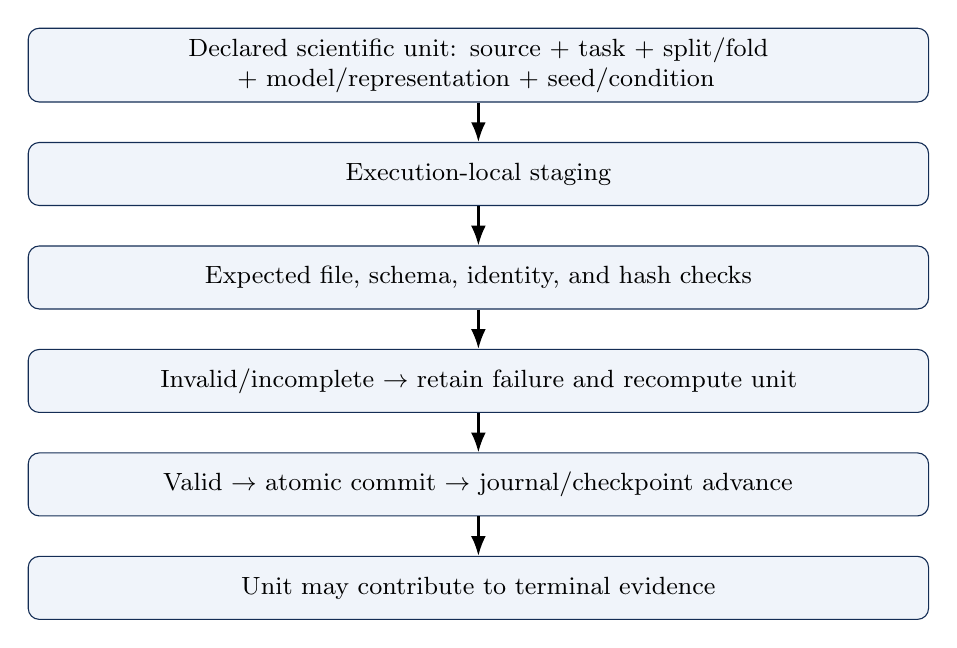
\begin{tikzpicture}[node distance=5mm,every node/.style={align=center,font=\small},stage/.style={draw=geoBlue,rounded corners,fill=geoLight,text width=11.2cm,minimum height=0.8cm}]
\node[stage] (a) {Declared scientific unit: source + task + split/fold + model/representation + seed/condition};
\node[stage,below=of a] (b) {Execution-local staging};
\node[stage,below=of b] (c) {Expected file, schema, identity, and hash checks};
\node[stage,below=of c] (d) {Invalid/incomplete $\rightarrow$ retain failure and recompute unit};
\node[stage,below=of d] (e) {Valid $\rightarrow$ atomic commit $\rightarrow$ journal/checkpoint advance};
\node[stage,below=of e] (f) {Unit may contribute to terminal evidence};
\foreach \x/\y in {a/b,b/c,c/d,d/e,e/f}{\draw[-{Latex[length=2.5mm]},thick] (\x)--(\y);}
\end{tikzpicture}
\caption{Only complete contract-valid units advance accepted execution state. A visible partial file is not evidence that the scientific unit completed.}
\end{figure}

\begin{governingrule}[Verified continuation]
Resume from the last verified scientific boundary, not from the last visible file.
\end{governingrule}

\section{Observed continuity and recovery}
The JARVIS replay was interrupted and resumed under the same execution identity; an incomplete staging unit was rejected and recomputed rather than merged or duplicated. The Materials Project replay also used a later resume launch while retaining only verified complete units. Separately, a controlled-fixture recovery matrix terminated real child processes at 11 declared fault boundaries and recovered each fixture to three unique committed units. These are controller fault-injection results, not 11 scientific experiments. A reported JARVIS zero-commit launch-envelope failure was not promoted into this measured register because a definitive run-local receipt was not isolated.

Fresh means a new identity with no predecessor work reused. Resume continues the same identity from verified commits. Repeat is a separately identified execution under the declared same environment where applicable. Replay is a new predecessor-linked identity compared under declared contracts. \textbf{Resume is not replication. Replay is not automatically external replication.}

\section{Calendar time, active execution, and a shared workstation}
The principal workstation was a shared personal machine rather than a dedicated compute node. Jobs were scheduled around ordinary availability, so calendar duration is much longer than active execution spans. The workstation remained available for ordinary use during parts of the programme; background load was uncontrolled and is not a performance benchmark.

Elapsed run time is launcher/process duration where a terminal receipt supports it. Summed unit wall time adds unit durations and can exceed elapsed time under parallelism. Committed-unit span runs from first to final accepted commit and can exclude setup or packaging. Calendar elapsed includes review, interruption, ordinary use, and unknown gaps and must not be called runtime. Spatial V0.6.1's 20.67 h fresh and 16.20 h replay values are committed-unit spans.

\begin{center}\small\ttfamily
[RUN] -- [ordinary use/review] -- [RUN] -- [interrupt/checkpoint] -- [unavailable] -- [RESUME/RUN] -- [review] -- [REPLAY]
\end{center}
Scientific identity follows committed evidence, not continuous ownership of the computer.

\section{Replay does not update accepted science by itself}
Execution completion may update execution memory. It must not automatically upgrade the scientific claim. A chronologically separate post-replay demonstration first submitted an eligible claim without human confirmation: the gate refused it and wrote zero accepted scientific-memory objects. Explicit founder adjudication then wrote and read back exactly two bounded local claims: Matbench fitted-use versus retrained-removal disagreement under same-environment repeat, and Spatial bulk metric geometry under exact cross-view local replay. Engineering action remained NONE.

Attempts to strengthen Spatial shear polarity and Materials Project elasticity beyond their ceilings were refused with zero positive promotions. Spatial shear remained conditional because replay exactly reproduced the cross-view failure; Materials Project elasticity retained its mixed replay and admission HOLD.

\begin{center}\small\bfseries
EXECUTION $\rightarrow$ COMPARISON $\rightarrow$ MACHINE CANDIDATE $\rightarrow$ HUMAN ADJUDICATION $\rightarrow$ BOUNDED MEMORY UPDATE OR HOLD $\rightarrow$ READ-BACK
\end{center}
The human controls the evidence-state transition, not merely manuscript wording. A scientific-memory update is not fabrication, deployment, qualification, or regulatory permission.


\section{What remains unmeasured}
The programme does not establish universal efficiency, production throughput, energy
efficiency, external replication or human-labour savings. The source providers' DFT
corpora were not recomputed locally.

\chapter{Governance and Claim Authority}
\label{chap:governance}

\section{Why governance appears last}
Governance is introduced after the materials experiments, engineering decisions and execution evidence because it is the response to a problem revealed by the experiments.

The programme produced states such as high prediction with low retrained-removal consequence, positive null separation with negative absolute performance, source availability with unresolved admissibility, and numerical replay with byte divergence. Governance preserves the state of each evidence object and controls what may be claimed.

\begin{governingrule}
Governance does not create scientific evidence. It prevents evidence from being promoted beyond the state it has actually reached.
\end{governingrule}

\section{The evidence-to-authority chain}
The chain from public data to engineering authority is:
\begin{equation}
\text{availability} \rightarrow \text{admission} \rightarrow \text{viability} \rightarrow \text{reliability} \rightarrow \text{replay} \rightarrow \text{bounded authority}.
\end{equation}

No later gate repairs an earlier failed requirement.

\begin{table}[H]
\centering
\caption{Evidence-to-authority gates.}
\label{tab:authority-gates}
\begin{tabularx}{\textwidth}{L{0.18\textwidth}YY}
\toprule
\textbf{Gate} & \textbf{Operational question} & \textbf{Failure state} \\
\midrule
Availability & Does the source expose the required field or object? & Record absent or incomplete. \\
Admission & Are units, method, sign and semantics adequate? & Source hold. \\
Viability & Does the model pass absolute ($R^2>0$) and relative ($S>0$) doors? & Hold or refuse. \\
Reliability & Does descriptor explanation survive disturbances and retrained removal? & Bounded use or refusal. \\
Replay & Does execution satisfy required replay contracts? & Replay hold. \\
Authority & What action does the surviving evidence permit? & Bounded permission only. \\
\bottomrule
\end{tabularx}
\end{table}

\section{Allowed terminal evidence states}
The monograph uses four principal terminal states: \accepted{}, \bounded{}, \hold{}, and \refuse{}.

\section{Chapter conclusion}
Governance preserves the distinctions among data, evidence, interpretation, permission and authority. A result may influence an engineering decision only to the extent that the required evidence gates have survived.


% ============================================================
% CHAPTER 11
% ============================================================

\chapter{Discussion, Novelty and Closest Prior Work}
\label{chap:discussion}

\section{The central result}
The central result of this monograph is the experimental separation of several evidence objects that are often allowed to collapse into one another:
\begin{equation}
\begin{aligned}\text{prediction} &\neq \text{viability}, & \text{fitted use} &\neq \text{retrained dependence},\\ \text{availability} &\neq \text{admissibility}, & \text{repetition} &\neq \text{transfer}.\end{aligned}
\end{equation}

\section{Distinguishing three contribution classes}
To evaluate the contribution of this work, it is necessary to distinguish three distinct contribution classes:
\begin{enumerate}
\item \textbf{Scientific Contributions}: The conceptual separation of descriptor authority from fitted importance, the two-door model viability rule ($R^2>0$ and $S>0$), and source admission requirements prior to property fitting.
\item \textbf{Empirical and Failure-Witness Contributions}: The complete audit and replay of JARVIS-DFT (75,993 records), the adverse elasticity result in the Materials Project (154,377 records), the demonstration of the null-separation paradox, and the sealed 3,440-unit Matbench removal programme and separately identified 3,440-unit exact same-environment repeat.
\item \textbf{Research-Instrument Contributions}: The construction of atomic contract-bound scientific units, deterministic replay comparators, verified checkpoint recovery, and claim-addressable evidence lineage.
\end{enumerate}

\section{Closest prior method families}
Geatomica overlaps with and builds upon several established scientific fields:

Adjacent methods often address different evidence objects. The contribution here is
the explicit separation and interaction of those objects under one bounded scientific
programme. Table~\ref{tab:closest-methods} summarises primary concerns; it does not
assert that every implementation in an adjacent family is limited to one function.

\begin{table}[H]
\centering
\scriptsize
\caption{Closest method families and the evidence object kept separate in Geatomica.}
\label{tab:closest-methods}
\begin{tabularx}{\textwidth}{L{0.20\textwidth}YY}
\toprule
\textbf{Method family} & \textbf{Primary object reused} & \textbf{Object kept separately inspectable} \\
\midrule
XAI and attribution & Fitted feature use and local/global attribution & Retrained dependence and bounded mechanism claims \\
Feature-selection stability & Selection recurrence under resampling & Prediction viability and engineering permission \\
Uncertainty quantification & Predictive uncertainty or confidence & Source admission and evidence authority \\
Applicability domain and OOD & Population and transfer boundary & Semantic admission and downstream action \\
Benchmark suites & Standard tasks, splits and metrics & Claim ceilings when evidence objects disagree \\
FAIR and provenance \cite{wilkinson2016fair,w3c2013prov} & Traceability, stewardship and lineage & Whether traced evidence has earned admission or action \\
Research objects and workflow systems \cite{soiland2022rocrate,koster2012snakemake,ditommaso2017nextflow} & Packaging, execution and reconstruction & Resume/replay meaning and accepted scientific state \\
Engineering assurance & Structured argument and failure containment & Empirical scientific gate results \\
Model governance \cite{tabassi2023airmf} & Lifecycle and organisational risk & Scientific evidence state before organisational promotion \\
\bottomrule
\end{tabularx}
\end{table}

\subsection{Feature importance and attribution}
Attribution algorithms such as SHAP \cite{lundberg2017unified}, LIME \cite{ribeiro2016why}, and Gini/permutation importance rank feature contributions within a fitted model. Geatomica demonstrates that fitted feature attributions do not establish retrained dependence or physical necessity. By placing fitted attributions beside retrained removal and multi-axis disturbance, Geatomica distinguishes features that a specific model uses from features that are associated with retrained-removal consequence under the declared representation.

\subsection{Feature-selection stability}
Stability selection \cite{meinshausen2010stability} evaluates the consistency of selected feature sets across subsamples. Geatomica incorporates stability analysis into a broader materials-assurance programme by measuring explanatory persistence under noise injection, population splitting, and cross-source transfer boundaries.

\subsection{Applicability domains and out-of-distribution robustness}
Quantitative structure-property relationship (QSPR) applicability domains \cite{tropsha2010best} define the chemical space where model predictions remain valid. Geatomica operationalizes population boundaries for both predictive accuracy and explanatory stability, refusing to authorize engineering actions when candidates cross structural or compositional boundaries.

\subsection{Uncertainty Quantification (UQ)}
Uncertainty quantification methods \cite{abdar2021review} estimate prediction variance and model confidence. Geatomica complements UQ by measuring evidence sufficiency---determining whether an uncertainty bound permits specific engineering actions (such as screening, escalation, or physical testing).

\subsection{Materials benchmark suites}
High-throughput materials repositories such as AFLOW \cite{curtarolo2012aflowlib}, OQMD \cite{saal2013materials}, and Matbench \cite{dunn2020benchmarking} provide standardized evaluation datasets. Geatomica operates inside these benchmark datasets while demonstrating that high benchmark scores cannot repair underlying source admission failures or unverified target definitions.

\subsection{Workflow provenance and scientific reproducibility}
Reproducible research standards \cite{stodden2014implementing, goble2014better, wilkinson2016fair} emphasize computational provenance. Geatomica connects cryptographic execution receipts directly to manuscript claim ceilings, enforcing fail-closed decision rules when execution logs are incomplete or non-reproducible.

\subsection{Engineering software assurance}
In contrast to purely predictive materials ML models \cite{ramprasad2017machine, merchant2023scaling}, Geatomica draws upon safety-case and software-assurance principles \cite{leveson2011engineering, kelly1998arguing, hatcliff2014rationale}. It is designed as an assurance layer that bounds model authority before predictions reach engineering workflows.

\section{The novelty claim}
The novelty claim of Geatomica is combinational: it brings together source admission, absolute/relative viability, descriptor-response testing, retrained removal, multi-contract replay, and bounded engineering permission into a single fail-closed architecture.

The novelty claim concerns the composition and explicit separation of these evidence
objects, not the invention of each constituent method family.

\section{Chapter conclusion}
The contribution lies in ensuring no single evidence object can impersonate another when a materials model begins to influence engineering decisions.


% ============================================================
% CHAPTER 12
% ============================================================

\chapter[Limitations, Threats and Future Falsification]{Limitations, Threats to Validity and Future\\ Falsification Programme}
\label{chap:limitations}

\section{Limitations define the present result}
Geatomica has demonstrated a materials-assurance method across large public datasets, multiple model families, and governed replays. It has not yet demonstrated physical causal discovery, experimental transfer, or universal descriptor hierarchy.

\section{Falsification programme}
Future work should prioritize 10 targeted falsification experiments: matched full-feature sham refits; alternative model families for the removal experiment; direct grouped or conditional fitted perturbation; tensor- and method-resolved Materials Project elasticity reconstruction; external clean-room reproduction; cross-platform replay; physical materials validation; a prospective industrial decision trial; authority-threshold sensitivity; and the first genuine non-materials-domain instantiation of the portable control logic.

\section{Chapter conclusion}
The strongest next work is not internal expansion, but an attempt to break current claims through new sources, spatial models, and physical measurements.


% ============================================================
% CONCLUSION
% ============================================================

\clearpage



\chapter*{Conclusion}
\addcontentsline{toc}{chapter}{Conclusion}
\label{chap:conclusion}

Materials engineers rarely receive the whole process; they receive what remains. A microstructure, a fracture surface, a calculated database record, or a trained machine-learning model is a surviving structure.

Geatomica emerged from the empirical demonstration that prediction is not viability, importance is not necessity, availability is not admissibility, and replay is not universal truth. Its purpose is not to declare every model trustworthy, but to measure the boundary of trust and issue a smaller, clearer, and more defensible permission to act.

\textbf{If you remember one thing:} no computational evidence object should be allowed to stand in for a stronger one that has not actually been tested.


% ============================================================
% APPENDICES
% ============================================================

\clearpage
\appendix

\chapter{Experiment Register}

\begin{longtable}{p{0.20\textwidth}p{0.19\textwidth}p{0.23\textwidth}p{0.27\textwidth}}
\toprule
Route & Scale & Replay state & Principal outcome \\
\midrule
JARVIS tabular & 48 + 48 units & 28,248 cells; max delta $\sim1.07\times10^{-14}$ & viable carrier with target/model/population dependence \\
Materials Project & 64 + 64 units & mixed; 916 strict exceedances, all elastic & admission and viability holds retained \\
Matbench removal & 3,440 + 3,440 units & 65,740 cells exact & fitted importance diverged from retrained removal \\
Spatial persistence & 256 materials & sealed predecessor route & six-bin angle advantage failed to persist \\
Spatial V0.5 DOE & 256 + 256 units & byte/metadata/numeric PASS & metric geometry strongest compact block \\
Spatial V0.6.1 & 576 + 576 units & 1,728 byte-identical pairs; 927,361 cells exact & bulk geometry confirmed; shear polarity conditional \\
\bottomrule
\end{longtable}

\chapter{Claim-to-Evidence Matrix}
\label{appendix:claim-matrix}

\begin{longtable}{L{0.39\textwidth}L{0.18\textwidth}L{0.33\textwidth}}
\caption{Claim-to-evidence matrix.} \label{tab:claim-evidence-matrix} \\
\toprule
\textbf{Claim} & \textbf{State} & \textbf{Boundary} \\
\midrule
\endfirsthead
\toprule
\textbf{Claim} & \textbf{State} & \textbf{Boundary} \\
\midrule
\endhead
JARVIS non-null predictive structure & Supported & Within frozen JARVIS populations and representations. \\
JARVIS numerical replayability & Supported & Local locked replay at $10^{-10}$ tolerance. \\
Target-specific descriptor enhancement & Supported & Within frozen non-leakage register. \\
MP formation energy & Bounded support & Population-level recurrence across sources. \\
MP raw elasticity physical use & Refused & Extreme and negative values triggered scrutiny; unresolved tensor-, method-, and convention-level evidence prevented the strongest physical-use category under the declared admission rubric. \\
Importance proves necessity & Not authorised & Matbench establishes an exactly repeated measurement disagreement, not physical necessity or causal irrelevance. \\
\bottomrule
\end{longtable}


\chapter{Reproducibility, Runtime and Hardware Register}

\begin{longtable}{p{0.20\textwidth}p{0.18\textwidth}p{0.22\textwidth}p{0.29\textwidth}}
\toprule Route & Runtime & Comparison & State \\
\midrule
JARVIS & $\sim$9.93 h fresh & 28,248 cells; 60/192 raw files byte-divergent & numerical PASS within frozen tolerance \\
Materials Project & not recovered & 37,924 cells; 916 exceedances & mixed replay; elastic hold retained \\
Matbench & 19.16 / 20.60 h & 65,740 cells & exact numerical and semantic identity \\
Spatial V0.5 & 9.64 / 9.10 min & 256 + 256 units & byte, metadata and numerical identity \\
Spatial V0.6.1 & 20.67 / 16.20 h committed spans & 1,728 output pairs; 927,361 cells & byte, metadata and numerical identity; max delta 0 \\
\bottomrule
\end{longtable}

The principal workstation was an AMD Ryzen 7 5800X with 32 GB RAM and an installed
RTX 3060. The reported tabular routes were CPU-based. Same-environment replay is not
external replication.


\chapter{Scientific Reproduction Configuration Register}
\label{app:scientific-config}
This appendix consolidates the claim-relevant scientific settings. It is a method register, not a release of the private execution or authority machinery.

\section*{JARVIS-DFT audit}
\begin{longtable}{p{0.23\textwidth}p{0.67\textwidth}}
\toprule Item & Frozen scientific configuration\\\midrule
Source and cohorts & JARVIS-DFT \texttt{dft\_3d}; source census 75,993; four-property common cohort 23,824; target-specific admissible cohorts retained separately.\\
Targets & Formation energy per atom, band gap, bulk modulus $K_V$, shear modulus $G_V$.\\
Representations & Common leakage-restricted descriptor lane and target-specific lane under the frozen protocol.\\
Models & Ridge, Random Forest, Extra Trees and HistGradientBoosting under the frozen source protocol.\\
Population and scale & Seeds 11, 23, 37; row-random, composition-group and chemical-system splits; 2k, 5k, 10k and full-data scales.\\
Controls & Noise, dropout, feature shuffle, descriptor removal and paired target-permutation nulls.\\
Replay & 48 fresh + 48 replay units; 28,248 compared numeric cells; maximum absolute difference approximately $1.07\times10^{-14}$.\\
\bottomrule
\end{longtable}

\section*{Materials Project audit}
\begin{longtable}{p{0.23\textwidth}p{0.67\textwidth}}
\toprule Item & Frozen scientific configuration\\\midrule
Source & Materials Project checkpoint dated 28 July 2026; approximately 154,377 unique source records. Elastic route: 13,028 source records; 13,021 common-cohort records.\\
Targets & Formation energy, band gap, bulk modulus and shear modulus; elastic viability analysis keeps bulk and shear separate.\\
Representations & Eleven common descriptors and sixteen target-specific descriptors.\\
Preprocessing & All four model families used the same fold-local preprocessing: numeric coercion and median imputation followed by StandardScaler; categorical crystal-system values received most-frequent imputation and dense one-hot encoding with unknown categories ignored. All transformers were fitted on the training partition only.\\
Models & Ridge ($\alpha=1$); Random Forest (200 trees, minimum leaf 2); Extra Trees (300 trees, minimum leaf 2); HistGradientBoosting (250 iterations, depth 6, learning rate 0.05).\\
Population and scale & Seeds 11, 23, 37; 80/20 row-random, reduced-composition-group and chemical-system-group splits; 2k, 5k, 10k and full scales.\\
Null & At full scale, each eligible valid cell was paired with the mean $R^2$ across 30 target-permutation refits. Training targets were permuted while the held-out targets and other declared coordinates remained fixed.\\
Metrics and replay & \texttt{sklearn.metrics.r2\_score} and MAE. 64 fresh + 64 replay units; 37,924 compared numeric cells; 916 strict tolerance exceedances, all elastic.\\
\bottomrule
\end{longtable}

\section*{Matbench importance/removal audit}
\begin{longtable}{p{0.23\textwidth}p{0.67\textwidth}}
\toprule Item & Frozen scientific configuration\\\midrule
Tasks and size & \texttt{matbench\_mp\_e\_form} (132,752), \texttt{matbench\_mp\_gap} (106,113), \texttt{matbench\_log\_kvrh} (10,987), and \texttt{matbench\_log\_gvrh} (10,987); official five folds.\\
Representation & 142 Magpie composition descriptors. Fold-local median imputation and StandardScaler fitted on training data only.\\
Model & scikit-learn 1.8.0 MLPRegressor; hidden layers 128/64; ReLU; Adam; $\alpha=10^{-4}$; initial learning rate $10^{-3}$; maximum 300 iterations; early stopping; validation fraction 0.15; patience 20; random state 11.\\
Fitted importance & Held-out permutation importance, five repeats, fixed random state; fold-level aggregation.\\
Removal & Complete refitting after each individual descriptor removal and after each of 29 declared group removals; preprocessing refitted within the changed representation.\\
Comparison & Spearman rank association, top-10 overlap, MAE change and target-level group summaries.\\
Repeat & 3,440 fresh + 3,440 repeat units; two bounded CPU workers; 65,740 compared numeric cells; maximum difference 0.\\
\bottomrule
\end{longtable}

\section*{Spatial V0.5 representation DOE}
\begin{longtable}{p{0.23\textwidth}p{0.67\textwidth}}
\toprule Item & Frozen scientific configuration\\\midrule
Cohort and targets & Frozen 256-record JARVIS cohort; bulk modulus $K_V$ and shear modulus $G_V$; contiguous JID-ordered four-fold split.\\
Predictor & \texttt{sklearn.linear\_model.Ridge(alpha=1e-6)}; seed 20260809.\\
Baseline & Mean, standard deviation, minimum and maximum atomic number plus mean and standard deviation atomic mass.\\
Factors & A: symmetry/regime; B: coordination topology; C: continuous metric geometry; D: repaired six-bin angular geometry; E: electronegativity/polarity proxies.\\
Design and controls & Full $2^5$ factorial, 32 configurations, 256 scientific units per execution; translation, rotation, atom-permutation and supercell controls; tolerance $10^{-8}$.\\
Replay & Required; 256 fresh + 256 replay units; byte, semantic and numerical identity passed.\\
\bottomrule
\end{longtable}

\section*{Spatial V0.6.1 confirmation}
\begin{longtable}{p{0.23\textwidth}p{0.67\textwidth}}
\toprule Item & Frozen scientific configuration\\\midrule
Cohort and model & Same frozen 256-record cohort and Ridge($\alpha=10^{-6}$).\\
Population views & JID-order contiguous four-fold view and chemical-system-group four-fold view; decisions kept separate.\\
Configurations & BASE, B, E, B+E, C, C+E and dimension-matched sham configurations defined before execution.\\
Null and shams & Three paired-null seeds (20260809--20260811); training target only permuted. Deterministic target-blind within-partition feature shams; no train/test movement.\\
Decision rules & Bulk C required $\Delta R^2\ge0.05$ against BASE and SHAM\_C in each view with at least 3/4 positive folds. Shear E-over-C required $\Delta R^2\ge0.02$ against C and C+SHAM\_E in each view with at least 3/4 positive folds.\\
Controls and replay & Representation tolerance $10^{-8}$; same-environment replay tolerance $10^{-10}$; 576-unit ordered plan; 576 fresh + 576 replay; 1,728 output pairs; 927,361 numeric cells; maximum replay difference 0.\\
\bottomrule
\end{longtable}

\paragraph{Unresolved reproduction fields.} Exact provider-side generation settings for third-party source corpora remain governed by the source providers. Public reproduction begins from the cited source datasets and frozen cohort/split identities; it does not reproduce the providers' underlying first-principles calculations.

\chapter{Public Evidence Package}
\label{appendix:public-evidence}

\begin{evidencebox}[Release condition]
No figure, table or numerical headline remains in the public monograph unless it can be traced to a machine-readable evidence artefact.
\end{evidencebox}


\chapter{Evidence Verification Statement}
\section{Verified publication state}
The public evidence edition was checked against the executable metric implementation,
sealed execution and replay receipts, accepted scientific adjudications and the final
Spatial V0.6.1 assessment. The reported $R^2$ definition follows the evaluated-set
target mean used by \texttt{sklearn.metrics.r2\_score}. Matbench fresh/repeat evidence,
Materials Project same-denominator viability results and Spatial V0.6.1 fresh/replay
states were reconciled across the monograph and companion papers.

The verification establishes internal consistency and same-environment replay states.
It does not constitute peer review, external replication, physical qualification,
regulatory approval or authority for 512-material scaling.


\chapter*{Declarations}
\addcontentsline{toc}{chapter}{Declarations}

\textbf{Funding.} This research was conducted independently without dedicated external research grant funding.

\textbf{Competing interests.} The author is founder of a venture developing software and services related to scientific evidence assurance and engineering decision support described in this work.

\textbf{Data and code availability.} The underlying source datasets are available through JARVIS-DFT, the Materials Project and Matbench under their respective access and licence terms. The maintained public research compendium is available at \href{https://github.com/JosephMaxwell02/materials-ml-failure-analysis}{github.com/JosephMaxwell02/materials-ml-failure-analysis}; its archived v1.0.0 release is \href{https://doi.org/10.5281/zenodo.21919563}{doi:10.5281/zenodo.21919563}. Compendium scripts reconstruct readouts from accepted derived tables. A separate \href{https://github.com/JosephMaxwell02/materials-ml-scientific-verification-rerunner}{scientific verification rerunner}, archived at \href{https://doi.org/10.5281/zenodo.21939447}{doi:10.5281/zenodo.21939447}, performs selected bounded fitting calculations; it does not rerun every published campaign. Exact historical Materials Project inputs are not redistributed.

\textbf{Rights.} Copyright \textcopyright{} 2026 Joseph Maxwell. All rights reserved unless an individual file explicitly states otherwise. Public availability permits reading, citation and scholarly inspection under applicable law; it does not grant an open-source licence or relicense third-party data.

\textbf{AI assistance.} AI and coding tools assisted code development, critique, diagnosis, evidence organisation, and manuscript preparation. They did not generate source target data. Frozen analyses were executed by conventional scientific software under declared protocols, and scientific interpretations and conclusions were reviewed by the author.

\textbf{Author contribution.} Joseph Maxwell is the sole human author and research lead of the reported programme.


% ============================================================
% REFERENCES (THEBIBLIOGRAPHY)
% ============================================================

\clearpage
\begin{thebibliography}{26}
\addcontentsline{toc}{chapter}{References}

\bibitem{choudhary2020joint}
Choudhary, K., Garrity, K. F., Reid, A. C., DeCost, B., Biacchi, A. J., Hight Walker, A. R., ... \& Tavazza, F. (2020). The joint automated repository for various integrated simulations (JARVIS) for data-driven materials design. \emph{npj Computational Materials}, 6, 173.

\bibitem{jain2013commentary}
Jain, A., Ong, S. P., Hautier, G., Chen, W., Richards, W. D., Dacek, S., ... \& Persson, K. A. (2013). Commentary: The Materials Project: A materials genome approach to accelerating materials innovation. \emph{APL Materials}, 1(1), 011002.

\bibitem{dunn2020benchmarking}
Dunn, A., Wang, Q., Ganose, A., Dopp, D., \& Jain, A. (2020). Benchmarking materials property prediction methods: the Matbench test set and Automatminer reference algorithm. \emph{npj Computational Materials}, 6, 138.

\bibitem{ward2016general}
Ward, L., Agrawal, A., Choudhary, A., \& Wolverton, C. (2016). A general-purpose machine learning framework for predicting properties of inorganic materials. \emph{npj Computational Materials}, 2(1), 16028.

\bibitem{lundberg2017unified}
Lundberg, S. M., \& Lee, S. I. (2017). A unified approach to interpreting model predictions. \emph{Advances in Neural Information Processing Systems}, 30, 4765--4774.

\bibitem{ribeiro2016why}
Ribeiro, M. T., Singh, S., \& Guestrin, C. (2016). "Why should I trust you?": Explaining the predictions of any classifier. \emph{Proceedings of the 22nd ACM SIGKDD International Conference on Knowledge Discovery and Data Mining}, 1135--1144.

\bibitem{meinshausen2010stability}
Meinshausen, N., \& B{\"u}hlmann, P. (2010). Stability selection. \emph{Journal of the Royal Statistical Society: Series B (Statistical Methodology)}, 72(4), 417--473.

\bibitem{tropsha2010best}
Tropsha, A. (2010). Best practices for QSAR model development, validation, and exploitation. \emph{Molecular Informatics}, 29(6-7), 476--488.

\bibitem{abdar2021review}
Abdar, M., Pourpanah, F., Hussain, S., Rezazadegan, D., Liu, L., Ghavamzadeh, M., ... \& Nahavandi, S. (2021). A review of uncertainty quantification in deep learning: Techniques, applications and challenges. \emph{Information Fusion}, 76, 243--297.

\bibitem{curtarolo2012aflowlib}
Curtarolo, S., Setyawan, W., Wang, S., Xue, J., Yang, K., Taylor, R. H., ... \& Sanvito, S. (2012). AFLOWLIB.ORG: A distributed repository of high-throughput band structures and total energies. \emph{Computational Materials Science}, 58, 227--235.

\bibitem{saal2013materials}
Saal, J. E., Kirklin, S., Aykol, M., Meredig, B., \& Wolverton, C. (2013). Materials design at the Materials Genome Initiative scale: The Open Quantum Materials Database (OQMD). \emph{JOM}, 65(11), 1501--1509.

\bibitem{xie2018crystal}
Xie, T., \& Grossman, J. C. (2018). Crystal graph convolutional neural networks for an accurate and interpretable prediction of material properties. \emph{Physical Review Letters}, 120(14), 145301.

\bibitem{chen2019graph}
Chen, C., Ye, W., Zuo, Y., Zheng, C., \& Ong, S. P. (2019). Graph networks as a universal machine learning framework for molecules and crystals. \emph{Chemistry of Materials}, 31(9), 3564--3572.

\bibitem{stodden2014implementing}
Stodden, V., Leisch, F., \& Peng, R. D. (2014). \emph{Implementing Reproducible Research}. CRC Press.

\bibitem{goble2014better}
Goble, C. (2014). Better software, better research. \emph{IEEE Internet Computing}, 18(5), 4--8.

\bibitem{wilkinson2016fair}
Wilkinson, M. D., Dumontier, M., Aalbersberg, I. J., Appleton, G., Axton, M., Baak, A., ... \& Mons, B. (2016). The FAIR Guiding Principles for scientific data management and stewardship. \emph{Scientific Data}, 3, 160018.

\bibitem{w3c2013prov}
W3C Provenance Working Group. (2013). \emph{PROV-O: The PROV Ontology}. W3C Recommendation, 30 April 2013. \url{https://www.w3.org/TR/prov-o/}

\bibitem{soiland2022rocrate}
Soiland-Reyes, S., Sefton, P., Crosas, M., et al. (2022). Packaging research artefacts with RO-Crate. \emph{Data Science}, 5, 97--138. \url{https://doi.org/10.3233/DS-210053}

\bibitem{koster2012snakemake}
Koster, J., \& Rahmann, S. (2012). Snakemake---a scalable bioinformatics workflow engine. \emph{Bioinformatics}, 28(19), 2520--2522. \url{https://doi.org/10.1093/bioinformatics/bts480}

\bibitem{ditommaso2017nextflow}
Di Tommaso, P., Chatzou, M., Floden, E. W., Prieto Barja, P., Palumbo, E., \& Notredame, C. (2017). Nextflow enables reproducible computational workflows. \emph{Nature Biotechnology}, 35, 316--319. \url{https://doi.org/10.1038/nbt.3820}

\bibitem{tabassi2023airmf}
Tabassi, E. (2023). \emph{Artificial Intelligence Risk Management Framework (AI RMF 1.0)}. NIST AI 100-1. \url{https://doi.org/10.6028/NIST.AI.100-1}

\bibitem{ramprasad2017machine}
Ramprasad, R., Batra, R., Pilania, G., Mannodi-Kanakkithodi, A., \& Kim, C. (2017). Machine learning in materials informatics: recent applications and prospects. \emph{npj Computational Materials}, 3, 54.

\bibitem{merchant2023scaling}
Merchant, A., Batzner, S., Schoenholz, S. S., Aykol, M., Cheon, G., \& Cubuk, E. D. (2023). Scaling deep learning for materials discovery. \emph{Nature}, 624(7990), 80--85.

\bibitem{leveson2011engineering}
Leveson, N. (2011). \emph{Engineering a Safer World: Systems Thinking Applied to Safety}. MIT Press.

\bibitem{kelly1998arguing}
Kelly, T. P. (1998). \emph{Arguing Safety: A Systematic Approach to Managing Safety Cases}. DPhil Thesis, University of York.

\bibitem{hatcliff2014rationale}
Hatcliff, J., Wassyng, A., Kelly, T., Comar, C., \& Jones, P. (2014). Certifiably safe software-dependent systems: challenges and directions. \emph{Future of Software Engineering Proceedings}, 182--200.

\end{thebibliography}

\end{document}
